%-------------------------------------------------------------------------%
%------------------------- Carga de paquetes -----------------------------%
%-------------------------------------------------------------------------%
\documentclass[12pt]{report}

\usepackage[a4paper,headheight=16pt,scale={0.8,0.8},hoffset=0cm]{geometry}
\usepackage[utf8]{inputenc}
\usepackage{setspace}
\usepackage{tikz}
% \usetikzlibrary{arrows}
\usepackage{enumerate}
\usepackage{amsmath}
\usepackage{amssymb}
\usepackage{amsthm}
\numberwithin{equation}{section}
\numberwithin{figure}{section}
\numberwithin{table}{section}
\usepackage{fancyhdr}
\usepackage[center,hang,bf]{caption}
\usepackage{float}
\usepackage{listings}
\usepackage{graphicx}
\usepackage{tabu}
\usepackage{subfig}
\usepackage{circuitikz}
\usepackage{wrapfig}
\usepackage{paralist}
\usepackage{booktabs}
\usepackage{multirow}
\usepackage{csquotes}
\usepackage{ragged2e}
\usepackage{chngcntr}
\makeatletter
\let\c@lofdepth\relax
\let\c@lotdepth\relax
\makeatother
\usepackage{chngcntr,tocloft}
\usepackage[spanish,shorthands=off]{babel}
\usetikzlibrary{patterns}
\usepackage{tikz}
\usetikzlibrary{shapes.symbols, positioning, calc}
\usetikzlibrary{shapes.geometric}
\usetikzlibrary{decorations.pathmorphing}
\usetikzlibrary{shadows.blur}

\usepackage{algorithm}
\usepackage{algorithmic}
\usepackage{amsfonts}
\usetikzlibrary{arrows.meta}

\usepackage{url}
\usepackage{hyperref} % Esto hace que los enlaces en la bibliografía sean interactivos (clicables)


\counterwithin*{figure}{section}
\counterwithin*{figure}{subsection}
\counterwithin*{figure}{subsubsection}
\addtolength{\cftfignumwidth}{2em}

\renewcommand{\thefigure}{%
  \ifnum\value{subsection}=0
    \thesection.\arabic{figure}%
  \else
    \ifnum\value{subsubsection}=0
      \thesubsection.\arabic{figure}%
    \else
      \thesubsubsection.\arabic{figure}%
    \fi
  \fi
}

\lstdefinelanguage{bash}{
  keywords={mkdir,cp,ln,ls,cd,tree},
  keywordstyle=\color{blue}\bfseries,
  sensitive=true,
  comment=[l]{\#},
  commentstyle=\color{gray}\ttfamily,
  stringstyle=\color{purple},
  morestring=[b]",
  morestring=[b]'
}


% --- Paleta de colores para código ---
\definecolor{bashKeyword}{HTML}{005F9E}  % Azul profesional
\definecolor{bashComment}{HTML}{6A737D}  % Gris suave
\definecolor{bashString}{HTML}{8F4E8B}   % Púrpura
\definecolor{bashBackground}{HTML}{F6F8FA}


\lstdefinestyle{bashstyle}{
  language=bash,
  basicstyle=\ttfamily\small,
  keywordstyle=\color{blue}\bfseries,
  commentstyle=\color{gray}\ttfamily,
  stringstyle=\color{purple},
  backgroundcolor=\color{gray!5},
  frame=single,
  rulecolor=\color{black!20},
  showstringspaces=false,
  breaklines=true,
  columns=fixed,
  keepspaces=true,
  escapeinside={(*@}{@*)}
}

%- para popner definiciones

\theoremstyle{definition} 
\newtheorem{definicion}{Definición}[chapter]

\usepackage{amsmath, amssymb, amsthm}


%-------------------------------------------------------------------------%
%------------------------- INICIO DEL DOCUMENTO --------------------------%
%-------------------------------------------------------------------------%
\begin{document}
\pagestyle{fancy}
\renewcommand{\headrulewidth}{0.3pt}
\renewcommand{\footrulewidth}{0.3pt}
\renewcommand{\thefootnote}{\Roman{footnote}}
\lhead{Conformal Predictión}
\chead{}
\rhead{Brian Fuentes}
%\lfoot{Qmetro}
\cfoot{}
\rfoot{\thepage}

%-------------------------------------------------------------------------%
%-------------------------- CARÁTULA -------------------------------------%
%-------------------------------------------------------------------------%
\begin{center}
%
\includegraphics[scale=0.4]{FIUBA.png}\\

\includegraphics[scale=0.4]{Uba_fiuba_ingenieria_logo.png}\\
\hfill\break
\large{\textsc{Departamento de Electrónica}}\\
\large{Laboratorio de proc. de señales y comunicaciones}
\end{center}

\vspace{0.1cm}
\begin{center}
\rule{1\textwidth}{1pt}
\setstretch{1}
\vspace{0.4cm}
\textbf{\large{\textsc{Predicción conforme en procesamiento de imágenes para problemas de ingeniería}}}
\large{\\Tesis de grado de Ingeniería Electrónica}
\end{center}

\begin{center}
\rule{1\textwidth}{1pt}
\end{center}
\vspace{-0.4cm}

\begin{center}
    {\textsc{Brian Fuentes}}
\end{center}

\begin{center}
    {\textsc{101785}}
\end{center}
\vspace{-0.5cm}
\newpage

%-------------------------------------------------------------------------%
%--------------------------- CONTENIDO -----------------------------------%
%-------------------------------------------------------------------------%
\begin{flushleft}

\setlength{\parindent}{12pt}
\newcommand{\norm}[1]{\left\lVert#1\right\rVert}

%%%%%%%%%%%%%%%%%%%%%%%%%%%%%%%%%%%%%%%%%%%%%%%%%%%%%%%%%%%%%%%%%%
\tableofcontents
\newpage


%%%%%%%%%%%%%%%%%%%%%%%%%%%%%%%%%%%%%%%%%%%%%%%%%%%%%%%%%%%%%%
\chapter{Introducción}

\label{sec:introduccion}

En la última década, las redes neuronales profundas y los modelos de aprendizaje automático han alcanzado un rendimiento extraordinario en tareas complejas de visión por computadora, procesamiento de imágenes médicas y modelado físico-matemático mediante redes guiadas por la física (\textit{Physics-Informed Neural Networks}, PINNs). A pesar de estos avances significativos, la implementación práctica de estas herramientas en entornos de alta responsabilidad y riesgo crítico (\textit{safety-critical}), tales como el diagnóstico médico, la Tomografía Optoacústica (TOA), la caracterización vascular, el procesamiento de imágenes cardíacas o la detección por radar THz, enfrenta un obstáculo fundamental: la falta de confiabilidad en sus estimaciones puntuales. En aplicaciones biomédicas e industriales, una predicción puntual única $y = \hat{f}(x)$ resulta inherentemente insuficiente para la toma de decisiones clínicas o técnicas. Un sistema automatizado no solo debe proporcionar una estimación, sino también comunicar de manera transparente su grado de incertidumbre y el nivel de confianza asociado, siendo vital comprender cuándo un modelo es proclive a cometer un error o a generar estructuras espurias (hallucinated features), es decir, patrones o características visuales que no están presentes en el objeto físico real pero que son introducidas por el proceso de inferencia o reconstrucción.

Las redes neuronales profundas modernas sufren sistemáticamente del fenómeno de excesiva confianza (\textit{overconfidence}) y mala calibración de sus salidas, tendiendo a asignar puntuaciones de probabilidad muy elevadas incluso en presencia de datos con ruido severo, artefactos de reconstrucción o entradas fuera de distribución (\textit{out-of-distribution}). Por otro lado, los métodos tradicionales de Cuantificación de Incertidumbre (\textit{Uncertainty Quantification}, UQ), tales como los enfoques Bayesianos (B-PINNs), el escalado de temperatura, el \textit{Monte Carlo Dropout} o los ensambles de redes, presentan limitaciones críticas relacionadas con elevados costos computacionales en inferencia, supuestos distribucionales Gaussianos no verificables y falta de garantías matemáticas para muestras finitas \cite{Yifan2025}. En modalidades como la Tomografía Optoacústica (TOA), donde la reconstrucción a partir de sinogramas es un problema inverso severamente mal condicionado y propenso a artefactos de visión limitada (\textit{limited-view}), una estimación de incertidumbre no calibrada puede inducir falsos positivos (simulando vasos sanguíneos inexistentes) o falsos negativos (ocultando estructuras patológicas).

Para superar estas deficiencias, esta investigación adopta el marco de la Predicción Conforme (\textit{Conformal Prediction}, CP) y el Control de Riesgo Conforme (\textit{Conformal Risk Control}, CRC). CP es un paradigma no paramétrico y agnóstico del modelo que actúa como una envoltura (\textit{wrapper}) \textit{post-hoc} sobre cualquier red neuronal previamente entrenada, transformando mediante un conjunto de calibración independiente las predicciones puntuales en conjuntos o intervalos de predicción con garantías matemáticas de cobertura válidas para muestras finitas ($1 - \alpha$) bajo el supuesto de intercambiabilidad. Por su parte, CRC extiende este principio a funciones de pérdida continuas para acotar formalmente el riesgo esperado por debajo de un umbral predefinido. La brecha de investigación abordada reside en la necesidad de adaptar formalmente CP y CRC a problemas de transporte de onda (TOA/PINNs), segmentación médica multi-estructura (como imágenes cardíacas) y sensores físicos (radar THz) mediante el diseño de funciones de no-conformidad y cuantiles locales (\textit{Local CP}) capaces de adaptarse a la heterocedasticidad espacial y a variaciones complejas de ruido.


El objetivo general de este trabajo es desarrollar y evaluar un marco unificado de cuantificación de incertidumbre y calibración \textit{post-hoc} basado en Predicción Conforme y Control de Riesgo Conforme, capaz de dotar a modelos de aprendizaje profundo y redes guiadas por la física de garantías estadísticas finitas y adaptabilidad local. Para validar la efectividad de este enfoque frente a distintos tipos de ruido y geometrías, el alcance experimental comprende tres escenarios de prueba diferenciados: la reconstrucción acústica en Tomografía Optoacústica (evaluando solucionadores FBPINNs y algoritmos DAS), la delimitación de estructuras anatómicas en imágenes médicas cardíacas con control de riesgo, y la estimación de señales físicas de alta frecuencia en sensores de radar THz.

Las principales contribuciones de esta investigación incluyen: la formulación de un marco de calibración ligero y agnóstico del modelo que garantiza la cobertura deseada del $(1-\alpha)\%$ sin requerir reentrenar la red base; la integración de cuantiles locales (\textit{Local CP}) para absorber la heterocedasticidad espacial en solucionadores neuronales de ecuaciones diferenciales; y una evaluación empírica rigurosa que demuestra cómo corregir la sobreconfianza estructural de estos modelos a través de métricas de cobertura, desviación promedio (ACD) y eficiencia en el tamaño de los conjuntos.

El trabajo se organiza secuencialmente comenzando con la fundamentación teórica de Predicción Conforme, intercambiabilidad y Control de Riesgo Conforme. 
A continuación, se desarrollan los principios físicos del pipeline de Tomografía Optoacústica, segmentación de imagenes cardiacas y detección por radar THz. Posteriormente, se detalla la metodología de calibración propuesta, las funciones de no-conformidad y los mapas de riesgo adaptativo. Finalmente, se presentan y discuten los resultados experimentales en las tres modalidades analizadas, sintetizando las conclusiones principales y las líneas futuras de desarrollo.



%$CORECCIONES$
%https://arxiv.org/pdf/1609.00451

%  Yo haría más teórica la intro. 
%  
%  Así como está no se entiende por que no eligiría un C=Y y ya está (tiene proba 1).
%  
%  Yo te diría que introduzcas con Least Ambiguos Classifier y demuestres en que sentido esto es óptimo.
%  
%  Lo podés leer en "Least Ambiguous Set-Valued Classifiers with Bounded Error Levels"  de Sadinle (teorema 1).
%  
%  Debe haber algo similar para regresión, hay que buscar y ampliar.
%  
%  Ya habiendo leído todo, me parece que falta un plan sobre que querés contar en este capítulo. Tiene que entenderse cuál es el hilo conector de la historia que estás contando

%Esta investigación aborda la problemática de la falta de confiabilidad y la excesiva confianza (overconfidence) de las redes neuronales modernas, las cuales operan habitualmente como "cajas negras" sin medidas rigurosas de incertidumbre.
%
%El objetivo central es el desarrollo y aplicación de marcos de trabajo basados en Predicción Conforme (CP) y Control de Riesgo Conforme (CRC) para transformar predicciones puntuales en conjuntos de predicción con garantías estadísticas de cobertura válidas para muestras finitas.
%
%
%\begin{itemize}
%    \item Nose....
%\end{itemize}




\chapter{Predicción conforme}
\section{Predicción Conforme}

En la práctica del aprendizaje automático y el modelado numérico, las estimaciones puntuales $\hat{y} = \hat{f}(x)$ resultan insuficientes para aplicaciones críticas, ya que no informan sobre la incertidumbre asociada a la predicción. La \textbf{Predicción Conforme} (o inferencia conforme) es un paradigma estadístico \textit{post-hoc} diseñado para envolver cualquier predictor puntual de "caja negra" y transformar sus salidas en \textbf{regiones de predicción} $\mathcal{C}(x)$ (conjuntos discretos o intervalos continuos) con garantías de cobertura estadísticamente rigurosas y no asintóticas.

\subsection{Cobertura y Eficiencia}

Dada una nueva observación de prueba $(X_{\text{test}}, Y_{\text{test}}) \in \mathcal{X} \times \mathcal{Y}$ y un nivel de error especificado por el usuario $\alpha \in (0, 1)$, se busca construir una región de predicción $\mathcal{C}(X_{\text{test}})$ que garantice la \textbf{validez} o \textbf{cobertura marginal}:

\begin{equation}
    \mathbb{P}\left( Y_{\text{test}} \in \mathcal{C}(X_{\text{test}}) \right) \ge 1 - \alpha
    \label{eq:marginal_cov}
\end{equation}

Sin embargo, exigir únicamente esta condición de cobertura es insuficiente. Un clasificador trivial que devuelva siempre el espacio completo de etiquetas $\mathcal{C}(x) = \mathcal{Y}$ (o la recta real $\mathcal{C}(x) = (-\infty, \infty)$ en regresión) satisface la cobertura con probabilidad 1, pero resulta completamente inútil desde el punto de vista práctico. Por lo tanto, la construcción de regiones de predicción óptimas requiere equilibrar dos objetivos contrapuestos:


\textbf{Cobertura:} Garantiza que la probabilidad de incluir la etiqueta verdadera sea de al menos $1 - \alpha$.

\textbf{Eficiencia e Informatividad:} Minimizar la extensión de la región predicha (el tamaño del conjunto en clasificación o la longitud del intervalo en regresión).

Además, de la \textbf{cobertura} se existen principalmente dos la \textbf{cobertura marginal}, definida por la ecuación \ref{eq:marginal_cov}, y la \textbf{cobertura condicional} \ref{eq:cond_cov}.

\begin{equation}
    \mathbb{P}\left( Y_{\text{test}} \in \mathcal{C}(X_{\text{test}}) \mid  X_{\text{test}}=x \right) \ge 1 - \alpha
    \label{eq:cond_cov}
\end{equation}

El cual exige que la garantia de $1 - \alpha$ se cumpla de forma independiente para cada valor de $\mathcal{X}$.

Esto puede generalizarse para otros tipos de coberturas derivadas de las ya mencionadas.

\begin{equation}
    \mathbb{P}\left( Y_{\text{test}} \in \mathcal{C}(X_{\text{test}}) \mid  E \right) \ge 1 - \alpha
    \label{eq:marginal_cov_E}
\end{equation}

\begin{itemize}
    \item \textbf{Marginal}: E = \{ \O \}  \text{Promedio global sobre todo el dataset de calibración y prueba} 

    \item \textbf{Condicional al objeto}: E = \{ $X_{text} = x$ \}  \text{Garantía puntual e independiente para cada coordenada $x$ específica} 

    \item \textbf{Condicional a la clase}: E = \{ $X_{text} = y$ \}  \text{Tasa de acierto garantizada por separado para cada categoría discreta $y$ (Sadinle, Vovk)-AGREGAR LA REF.}

    \item \textbf{Por grupos o atributos}: E = \{ $X_{text} \in \text{Grupo} \  g$ \}  \text{Cobertura garantizada de forma independiente para cada subgrupo demográfico o de sensores (Mondrian)-AGREGAR LA REF.}    
    
\end{itemize}


Si bien la cobertura condicional al objeto~\eqref{eq:marginal_cov_E} es el estándar ideal, puesto que asegura validez individualizada para cada entrada, se ha demostrado que garantizarla de forma exacta en muestra finita y libre de distribución es teóricamente imposible sin producir regiones de predicción triviales \cite{vock2012}. Por ello, en la práctica se recurre a relajaciones intermedias condicionando por clases, grupos o regiones espaciales.

\subsection{Regiones de Predicción Óptimas}

Para formalizar el sentido en que una región de predicción es óptima, se considera primero el caso teórico en el que la distribución conjunta $P(X,Y)$ es conocida.

\subsubsection{Caso Discreto: Clasificadores de Mínima Ambigüedad}

En clasificación multiclase con $\mathcal{Y} = \{1, \dots, K\}$, la eficiencia se mide mediante la \textbf{ambigüedad} $A(\mathcal{C})$, definida como el número esperado de etiquetas asignadas: $A(\mathcal{C}) = \mathbb{E}[|\mathcal{C}(X)|]$.

El Teorema de Optimalidad de Sadinle, Lei y Wasserman \cite{sadinle2018} demuestra que el clasificador basado en conjuntos que minimiza la ambigüedad sujeto a la restricción de cobertura objetivo está dado por los conjuntos de nivel de las probabilidades condicionales de clase $p(y|x) = \mathbb{P}(Y=y \mid X=x)$:

\begin{equation}
    \mathcal{C}^*(x) = \{y \in \mathcal{Y} : p(y|x) \ge t_\alpha\}
\end{equation}
donde $t_\alpha$ es el umbral que garantiza que la cobertura marginal sea exactamente $1 - \alpha$.




\subsubsection{Caso Continuo: Región de Longitud Mínima y Cuantiles Condicionales}
En problemas de regresión donde la respuesta es continua ($\mathcal{Y} = \mathbb{R}$), la medida de eficiencia relevante es la \textbf{longitud esperada del intervalo} (medida de Lebesgue):
\begin{equation}
    \min_{\mathcal{C}} \mathbb{E}[\text{Leb}(\mathcal{C}(X))] \quad \text{sujeto a} \quad \mathbb{P}(Y \in \mathcal{C}(X)) \ge 1 - \alpha
\end{equation}

Bajo condiciones de regularidad, la región de longitud mínima corresponde a las \textbf{Regiones de Alta Densidad} (HDR, \textit{High Density Regions}) definidas sobre la densidad condicional $f(y|x)$:
\begin{equation}
    \mathcal{C}^*(x) = \{y \in \mathbb{R} : f(y|x) \ge t_\alpha\}
\end{equation}

Cuando se restringe la salida a un único intervalo continuo con colas balanceadas $\frac{\alpha}{2}$, la solución óptima está delimitada por las funciones de \textbf{cuantiles condicionales verdaderos} $q_{\alpha / 2}(x)$ y $q_{1-\alpha / 2}(x)$:

\begin{equation}
    \mathcal{C}^*(x) = \left[ q_{\alpha/2}(x), \, q_{1-\alpha/2}(x) \right]
\end{equation}

\subsection{Inferencia Conforme en Muestra Finita}

En la práctica, las distribuciones verdaderas $p(y|x)$ o $q_\tau(x)$ no son conocidas y deben ser estimadas mediante modelos de aprendizaje automático (como redes neuronales, PINNs, etc). Evaluar directamente las regiones estimadas $\hat{\mathcal{C}}(x)$ sin calibración genera intervalos sin garantías estadísticas en muestra finita.

La \textbf{Predicción Conforme} resuelve este problema actuando como un envoltorio (\textit{wrapper}) no paramétrico que utiliza una muestra de calibración independiente para ajustar los umbrales de corte mediante \textbf{puntajes de no conformidad} $s(x, y)$. Bajo el único supuesto de \textbf{intercambiabilidad} de las observaciones, la inferencia conforme garantiza validez exacta en muestra finita:

\begin{equation}
    1-\alpha \le \mathbb{P}\left(Y_{\text{test}} \in \mathcal{C}(X_{\text{test}})\right) < 1-\alpha + \frac{1}{n+1}
    \label{eq:marg}
\end{equation}

donde $n$ es el número de muestras en el conjunto de calibración.
%-------------------------------------------------------------------------------------



Este no produce una predicción puntual $\hat{y}$ sino que produce una \textbf{región de predicción} $\mathcal{C}(x)$ (un conjunto o un intervalo) estadísticamente rigurosos.
De manera crucial, estos conjuntos son válidos en un sentido libre de distribución: poseen garantías explícitas y no asintóticas incluso sin asumir una distribución de los datos ni supuestos sobre el modelo.


Dada una muestra de prueba $X_{\text{test}}$, se dispone de un modelo previamente entrenado $\hat{f}(\cdot)$ que produce una estimación puntual $\hat{y} = \hat{f}(X_{\text{test}})$. El marco de la Predicción Conforme trata a este predictor como una "caja negra" (\textit{black-box}) totalmente agnóstica.

En la ecuación \ref{eq:marg} se da una garantia marginal es decir la probabilidad en promedio sobre la aleatoriedad de todo el conjunto de datos de calibración y de la nueva muestra de prueba $(X_{\text{test}}, Y_{\text{test}})$. Esto garantiza una tasa de acierto global del $(1-\alpha)\%$ a largo plazo.


Para calibrar el modelo y obtener esta garantía, se incorpora una etapa adicional al procedimiento tradicional de entrenamiento y evaluación: el \textbf{paso de calibración}. 






Este procedimiento no requiere asumir una distribución de 
probabilidad específica para los datos, 
sino únicamente el cumplimiento de la propiedad de \textbf{intercambiabilidad}.


\begin{definicion}[\textbf{Intercambiabilidad}]
Sean $Z_i = (X_i, Y_i)$ para $i = 1, \dots, n$ las muestras del conjunto de calibración y $Z_{n+1} = (X_{\text{test}}, Y_{\text{test}})$ una nueva muestra de prueba. Se dice que la secuencia $(Z_1, \dots, Z_{n+1})$ es \textbf{intercambiable} si para toda permutación $\pi$ del conjunto de índices $\{1, \dots, n+1\}$ se cumple que:
\begin{equation}
    (Z_1, \dots, Z_{n+1}) \stackrel{d}{=} (Z_{\pi(1)}, \dots, Z_{\pi(n+1)}),
\end{equation}
es decir, la distribución conjunta de las variables aleatorias permanece inalterada frente a cualquier reordenamiento de las observaciones.
\end{definicion}


Cabe destacar que la intercambiabilidad es una hipótesis más general que 
la condición clásica de variables independientes e idénticamente 
distribuidas (i.i.d.): toda secuencia i.i.d. es intercambiable, 
pero esta propiedad también se satisface bajo ciertas dependencias 
simétricas entre los datos.

La relevancia práctica de este supuesto radica en que, 
al evaluar cada par $(X_i, Y_i)$ mediante una función de discrepancia 
fija $s(X_i, Y_i)$ basada en el modelo previamente entrenado $\hat{f}$, 
las puntuaciones resultantes $(s_1, \dots, s_n, s_{n+1})$ preservan la 
intercambiabilidad. 
En consecuencia, la puntuación desconocida del ejemplo de prueba 
$s_{n+1}$ tiene exactamente la misma probabilidad de ocupar cualquier 
rango al ordenarse junto con las $n$ puntuaciones de calibración. 
Esto permite acotar el error esperado calculando simplemente el cuantil 
empírico $\hat{q}$ correspondiente al nivel $\lceil(n+1)(1-\alpha)\rceil$ 
sobre el conjunto de calibración. 
Este procedimiento general se formaliza 
en el Algoritmo~\ref{alg:conformal_prediction}.

\begin{algorithm}[H]
\caption{Proceso de Calibración en \textit{Marco general - Predicción Conforme}}
\label{alg:conformal_prediction}
\begin{algorithmic}[1] % El [1] numera cada paso automáticamente
    \STATE \textbf{Identificar}  y extraer del modelo previamente entrenado $\hat{f}$ una estimación inicial de confianza o incertidumbre (aún sin garantías estadísticas).
    
    \STATE \textbf{Definir} la función de puntuación $s(x,y) \in \mathbb{R}$, también llamada función de no conformidad (los puntajes más grandes definen un peor ajuste entre $x$ e $y$):
    \begin{itemize}
        \item $s(x,y)$ pequeño $\rightarrow$ buen ajuste.
        \item $s(x,y)$ grande $\rightarrow$ mal ajuste.
    \end{itemize}

    \STATE \textbf{Computar} $\hat{q}$ como el $\lceil(n+1)(1-\alpha)\rceil/n$-cuantil empírico de la función de puntuación evaluada en el conjunto de calibración:
    \begin{equation*}
        \hat{q} = \text{quantile}\left(s_1, \dots, s_n; \frac{\lceil(n+1)(1-\alpha)\rceil}{n}\right)
    \end{equation*}
    donde $s_i = s(X_i, Y_i)$ para $i=1, \dots, n$. Esto fija el tamaño del conjunto de predicción de forma que se garantiza una cobertura de $1-\alpha$.

    \STATE \textbf{Construir} la región o conjunto de predicción para un nuevo ejemplo $X_{\text{test}}$ utilizando el umbral $\hat{q}$:
    \begin{equation*}
        C(X_{\text{test}}) = \{ y : s(X_{\text{test}}, y) \le \hat{q} \}
    \end{equation*}
    Es decir, el conjunto incluye todos los valores de $y$ que poseen bajo puntaje según el umbral calibrado.
\end{algorithmic}
\end{algorithm}

El Algoritmo \ref{alg:conformal_prediction} define el \textit{Marco general} sobre el cual se construyen las distintas técnicas de \textit{Conformal Prediction}.

Este flujo establece una plantilla estándar de calibración: cualquier variante metodológica posterior se reduce, esencialmente, a proponer una definición particular para la función de puntuación de no conformidad $s(x,y)$ en el paso 2, manteniendo el resto del proceso de cuantificación de incertidumbre inalterado con distintas formas de calcular el percentil.

\begin{figure}[H]
    \centering
    \resizebox{1.04\textwidth}{!}{% <-- Cambia 0.95 para agrandar (ej. 1.0) o achicar
        %-------------------------------------------------------------------------%
% ARCHIVO: img_tex/diagrama.tex
% Arreglado con desactivación local para babel (spanish)
%-------------------------------------------------------------------------%
\shorthandoff{>} % Apaga el conflicto del español justo antes de empezar

\begin{tikzpicture}[
    scale=0.85, every node/.style={transform shape},
    % Estilos de los bloques centrales
    bloque/.style={rectangle, draw=gray!60, fill=blue!5, rounded corners=6pt, minimum width=3.5cm, minimum height=1.2cm, align=center, font=\small},
    % Estilo para el texto de las ecuaciones
    textoEq/.style={align=left, font=\small}
]

% 1. FONDOS DE COLORES (Izquierda Verde, Derecha Rosa)
\fill[green!8] (-9, -5.4) rectangle (0, 5.5); % Subí un poquito el fondo (de 5 a 5.5) para que tape la nueva ecuación
\fill[red!5] (0, -5.4) rectangle (9, 5.5);
\draw[gray!30, dashed] (0, -5) -- (0, 5.5); 

% 2. BLOQUES CENTRALES Y FLECHAS
% Agregamos la ecuación arriba de Data en (0, 4.9)
\node[font=\small] (dataset) at (0, 4.99) {$(X_i, Y_i)_{i=1,2,\dots, n}$};

\node[bloque] (data) at (0, 4) {Datos};
\node[bloque] (sistema) at (0, 1.5) {Sistema};
\node[bloque] (cp) at (0, -1.5) {CP \\ $\mathbb{P}(y_{\text{test}} \in \mathcal{C}(X_{\text{test}})) \ge 1-\alpha$};

\node[textoEq] at (0, -4.9) {$y_{test} \mathcal \in {C}(x_{test}) $};

% Flecha delgada desde la nueva ecuación hacia el bloque Data
\draw[->, gray!80, thin] (dataset) -- (data);

\draw[->, gray!80, thick] (data) -- (sistema);
\draw[->, gray!80, thick] (-1, 0.9) -- node[left, black] {$S_i$} (-1, -0.9);
\draw[->, gray!80, thick] (1, 0.9) -- node[right, black] {$\hat{y}_i$} (1, -0.9);
\draw[->, gray!80, thick] (cp) -- (0, -3.5);

% Parámetro alpha apuntando a CP
\draw[->, gray!80, thick] (-2.7, -1.5) node[left, black, font=\large] {$\alpha$} -- (cp);

% 3. LADO IZQUIERDO (Clasificación - Verde)
\node[textoEq] at (-6.5, 1.5) {
    $x_1 \rightarrow \{\hat{y}_2\}$ \\
    $x_2 \rightarrow \{\hat{y}_K\}$ \\
    $\vdots$ \\
    $x_N \rightarrow \{\hat{y}_1\}$
};

\node[textoEq] at (-6.5, -2) {
    $x_1 \rightarrow \{\hat{y}_2, \hat{y}_4, \hat{y}_6\}$ \\
    $x_2 \rightarrow \{\hat{y}_K, \hat{y}_5, \hat{y}_7, \hat{y}_8\}$ \\
    $\vdots$ \\
    $x_N \rightarrow \{\hat{y}_1\}$
};

\node[textoEq] at (-3, -4.2) {$\mathcal{C}(x_{i}) = \{\hat{y}_j, \hat{y}_n, \textcolor{green!60!black}{\hat{y}_{i}}, \hat{y}_k\}$};


% 4. LADO DERECHO (Regresión - Rosa)

% Gráfico Superior (Predicción puntual)
\begin{scope}[shift={(3.5, 0.5)}]
    \draw[->, thick] (0,0) -- (3,0);
    \draw[->, thick] (0,0) -- (0,2);
    % Curva azul de predicción
    \draw[blue!70!cyan, ultra thick] (0.2, 0.4) .. controls (1, 1.5) and (2, 1) .. (2.8, 1.8) node[right, black] {$\hat{y}$};
\end{scope}

% Gráfico Inferior (Intervalos de confianza / bandas)
\begin{scope}[shift={(3.5, -3.2)}]
    \draw[->, thick] (0,0) -- (3,0);
    \draw[->, thick] (0,0) -- (0,2);
    
    % Banda superior (azul claro)
    \draw[blue!30, thick] (0.2, 0.9) .. controls (1, 2) and (2, 1.5) .. (2.8, 2.3);
    % Banda inferior (azul claro)
    \draw[blue!30, thick] (0.2, 0.1) .. controls (1, 1.2) and (2, 0.7) .. (2.8, 1.3);
    % Curva central (gris gruesa)
    \draw[gray!50, line width=3pt] (0.2, 0.5) .. controls (1, 1.6) and (2, 1.1) .. (2.8, 1.8) node[right, black] {$\hat{y}$};
    
    % Etiquetas de las bandas I+ e I-
    \draw[red!70, thick] (2.4, 1.55) -- node[right, font=\tiny] {$I^+$} (2.4, 2.0);
    \draw[red!70, thick] (0.6, 0.5) -- node[right, font=\tiny] {$I^-$} (0.6, 0.85);
\end{scope}

\node[textoEq] at (3.5, -4.2) {$\mathcal{C}(x) = [\hat{y}(x) - I(x), \hat{y}(x) + I(x)]$};

\end{tikzpicture}

\shorthandon{>} % Lo vuelve a encender para que el resto del texto de tu informe funcione bien
    }
    \caption{Esquema general de Conformal Prediction para clasificación y regresión.}
    \label{fig:conformal_prediction}
\end{figure}

El Algoritmo~\ref{alg:conformal_prediction} está pensado usualmente para el caso de clasificación. Este flujo también se representa en la Figura~\ref{fig:conformal_prediction}, donde nos interesa analizar el lado izquierdo.

Para aplicarlo, se evalúan los datos en el modelo $\hat{f}$ con el fin de extraer sus predicciones o salidas (como la salida de \textit{softmax}) y calcular así las puntuaciones mediante la función de no conformidad seleccionada.

En el caso de clasificación, esta función puede definirse como $s(x_i,y_i) = \mathbf{P}(y_i=0 \mid x_i) = 1 - \mathbf{P}(y_i=1 \mid x_i)$ (con probabilidad denotada $\hat{\pi}(y \mid x)$), mientras que para la calibración en regresión puede utilizarse $s(x_i,y_i) = |y_i - \hat{y}|$. En ambos casos, la función de no conformidad se emplea para decidir qué muestras se incluyen dentro del conjunto de predicción.

\section{Split conformal predictión}

El esquema presentado en el Algoritmo~\ref{alg:conformal_prediction} corresponde a la variante 
conocida en la literatura como \textbf{Predicción Conforme Dividida} (\textit{Split Conformal Prediction}, 
SCP) o inductiva. Para comprender su relevancia práctica, es necesario contrastarla 
con la formulación original del marco, 
denominada \textbf{Predicción Conforme Completa} (\textit{Full Conformal Prediction}).

En la Predicción Conforme Completa no se reserva un conjunto de calibración separado, 
sino que se utilizan todos los datos disponibles para ajustar el modelo. 
Dado un conjunto de $n$ observaciones $\mathcal{D}_n = \{(X_i, Y_i)\}_{i=1}^n$ y 
una nueva entrada de prueba $X_{n+1}$, el método debe evaluar cada valor posible 
$y \in \mathcal{Y}$ como candidato para la etiqueta verdadera $Y_{n+1}$.  
Para cada candidato $y$, se construye un conjunto de datos aumentado $\mathcal{D}_n \cup \{(X_{n+1}, y)\}$, 
se reentrena el modelo predictivo $\hat{f}_y$ desde cero sobre ese conjunto y se recalculan todas 
las puntuaciones de no conformidad. Si bien este procedimiento aprovecha la totalidad 
de los datos para el entrenamiento, resulta computacionalmente prohibitivo en la práctica: 
en problemas de regresión continua exige ajustar el modelo infinitas veces por cada muestra 
de prueba, y en aprendizaje profundo vuelve inviable el costo de reentrenar redes 
neuronales complejas o redes guiadas por la física (PINNs) en tiempo de inferencia.

En este caso se parte de un set de datos $(X_i, Y_i)_{i=1,2, \dots n}$ el modelo se entrena una vez con los datos $(X_i, Y_i)_{i=1,2, \dots n/2}$ y se calibra con $(X_i,Y_i)_{i=n/2 + 1, \dots , n}$
Se considera el problema de regresión donde $\mathcal{X} \in \mathbb{R}$.



\begin{algorithm}[H]
\caption{SCP caso especial - regresión}
\label{alg:conformal_prediction_esp}
    \begin{algorithmic}[1] % Usa [1] para numerar cada línea, o déjalo vacío [] si no quieres números
        \STATE \textbf{Entrenamiento:} Utilizar los datos $(X_i, Y_i)$ para $i = 1, \dots, \frac{n}{2}$ para ajustar un modelo predictivo $\hat{f} : \mathcal{X} \to \mathbb{R}$.

        \STATE \textbf{Cálculo de residuos:} Para $i = \frac{n}{2} + 1, \dots, n$, calcular el residuo absoluto $S_i = |Y_i - \hat{f}(X_i)|$.

        \STATE \textbf{Cálculo del cuantil:} Ordenar los residuos $S_{\frac{n}{2}+1}, \dots, S_n$ en orden creciente, y definir $\hat{q}$ como el elemento de valor $\lceil(1 - \alpha)(\frac{n}{2} + 1)\rceil$ en la lista ordenada.
        Entonces, $\hat{q} = \text{quantile}\left(s_1, \dots, s_n; \frac{\lceil(n+1)(1-\alpha)\rceil}{n}\right)$.

        \STATE \textbf{Inferencia:} Devolver el intervalo de predicción $\mathcal{C}(X_{n+1}) = [\hat{f}(X_{n+1}) - \hat{q}, \hat{f}(X_{n+1}) + \hat{q}]$.
    \end{algorithmic}
\end{algorithm}

El algortimo \ref{alg:conformal_prediction_esp} a diferencia del algoritmo \ref{alg:conformal_prediction} el conjunto de prediccion devuelto es un intervalo $\mathcal{C}(X_{n+1}) = [\hat{f}(X_{n+1}) - \hat{q}, \hat{f}(X_{n+1}) + \hat{q}]$ el cual representa la incerteza alrededor de la prediccion $\hat{f}(X_{n+1})$ para el target $Y_{n+1}$.

El valor de $\hat{q}$ es una constante que se calcula con los datos de calibración $(X_i,Y_i)_{i=n/2, \dots, n}$ y en esos datos se eleigio $\hat{q}$ de forma que cumpla que los $Y_i$ esten contenidos en el intervalo una fracción de $1-\alpha$. siendo los datos iid luego cualquier nueva prediccion va a cumplir la garantia marginal.


\begin{algorithm}[H]
\caption{SCP caso general}
\label{alg:conformal_prediction_gen}
    \begin{algorithmic}[1]
    \STATE \textbf{Construcción de la función de puntuación:} Utilizar los datos $(X_i, Y_i)$ para $i = 1, \dots, n/2$ para construir una \textbf{score de no conformida} $s : \mathcal{X} \times \mathcal{Y} \to \mathbb{R}$.

    \STATE \textbf{Cálculo de puntuaciones:} Para $i = n/2 + 1, \dots, n$, calcular la puntuación $S_i = s(X_i, Y_i)$ para cada dato en el conjunto de calibración.

    \STATE \textbf{Cálculo del cuantil:} Ordenar las puntuaciones $S_{n/2+1}, \dots, S_n$ en orden creciente, y definir $\hat{q}$ como el cuantil empirico de nivel $\lceil(1 - \alpha)(\frac{n}{2} + 1)\rceil$ en la lista ordenada.

    \STATE \textbf{Inferencia:} Devolver el conjunto de predicción $\mathcal{C}(X_{n+1}) = \{y \in \mathcal{Y} : s(X_{n+1}, y) \leq \hat{q}\}$.
    \end{algorithmic}
\end{algorithm}

La intuición de $s(x, y)$ es que mide qué tan ``inusual'' es el punto $(x, y)$ basándose en un modelo ajustado con los datos de esta primera mitad.

En el Algoritmo~\ref{alg:conformal_prediction_gen} vemos que este método no es solo de regresión, sino que se ajusta a ambos casos (clasificación y regresión). En general, todas las variantes que veremos en las siguientes secciones también pueden aplicarse a ambos problemas de calibración.

\section{Puntuaciones de no conformidad}

Las \textbf{puntuaciones de no conformidad} constituyen el elemento central del marco de la Predicción Conforme. Formalmente, se definen mediante una función $s(x, y)$ diseñada de modo tal que valores más altos indiquen una mayor discrepancia entre el par $(x, y)$ y el comportamiento aprendido por el modelo en los datos de entrenamiento. En términos prácticos, esta función actúa como una métrica que cuantifica el error o la falta de ajuste del predictor frente a una observación dada.

Una propiedad destacable de este enfoque es su flexibilidad: es posible emplear prácticamente cualquier función de puntuación, ya que, siempre que se preserve la simetría respecto al orden de los datos, el procedimiento garantiza matemáticamente el nivel de cobertura marginal $1-\alpha$, independientemente de cuán preciso o deficiente sea el modelo base. Sin embargo, aunque la validez estadística está asegurada por construcción, la elección específica de $s(x, y)$ resulta determinante en la práctica. Una función de no conformidad bien diseñada permite aprovechar la información del predictor para generar conjuntos o intervalos de predicción más estrechos y precisos. En la literatura del área, esta cualidad de minimizar la amplitud o el tamaño del conjunto devuelto sin perder el nivel de cobertura exigido se denomina \textbf{eficiencia}.

\subsection{Funciones de puntuación en regresión}

En problemas de regresión, la cobertura marginal por sí sola resulta insuficiente, ya que un intervalo excesivamente amplio e inflexible podría cumplirla de forma trivial perdiendo toda utilidad práctica. Idealmente, un intervalo de predicción debe reflejar la incertidumbre local de los datos, ensanchándose en zonas de alta varianza (heterocedasticidad) y estrechándose en regiones más estables. Según cómo se defina la puntuación de no conformidad, se obtienen distintos grados de adaptabilidad.

La formulación más directa es la \textbf{puntuación por residuo absoluto}, definida como 

\begin{equation}
    s(x, y) = |y - \hat{f}(x)|.
\end{equation}

Al depender únicamente del error puntual sin ponderar la dispersión local, este criterio produce bandas de confianza de \textbf{ancho constante} alrededor de la predicción, dadas por $[\hat{f}(X_{n+1}) - \hat{q}, \, \hat{f}(X_{n+1}) + \hat{q}]$.

Para superar esta rigidez cuando la varianza del ruido no es constante, se recurre a la \textbf{puntuación por residuo escalado}, que normaliza el error mediante una estimación local de la dispersión $\hat{\sigma}(x)$:
\begin{equation}
    s(x, y) = \frac{|y - \hat{f}(x)|}{\hat{\sigma}(x)}.
\end{equation}
De este modo, el intervalo de predicción resultante adapta su amplitud según la incertidumbre estimada en cada punto:
\begin{equation}
    \mathcal{C}(X_{n+1}) = \hat{f}(X_{n+1}) \pm \hat{q}\,\hat{\sigma}(X_{n+1}).
\end{equation}

Una alternativa aún más flexible es la \textbf{Regresión Cuantílica Conforme} (\textit{Conformalized Quantile Regression}, CQR), que parte de estimaciones iniciales de cuantiles condicionales $[\hat{\tau}(x; \alpha/2), \, \hat{\tau}(x; 1 - \alpha/2)]$ para medir la distancia con signo del valor real $y$ respecto a dicho intervalo:
\begin{equation}
    s(x, y) = \max \left\{ \hat{\tau}(x; \alpha/2) - y, \, y - \hat{\tau}(x; 1 - \alpha/2) \right\}.
\end{equation}
Un valor positivo de $s(x,y)$ indica que el dato real quedó por fuera del intervalo estimado, mientras que un valor negativo señala que cayó en su interior. Tras calibrar el cuantil empírico $\hat{q}$ sobre estas puntuaciones, el conjunto de predicción final se obtiene ajustando ambos extremos del intervalo inicial:
\begin{equation}
    \mathcal{C}(X_{n+1}) = \left[ \hat{\tau}(X_{n+1}; \alpha/2) - \hat{q}, \, \hat{\tau}(X_{n+1}; 1 - \alpha/2) + \hat{q} \right].
\end{equation}
Este enfoque no paramétrico permite construir \textbf{intervalos asimétricos y adaptativos} a la distribución local de los datos sin asumir simetría en los residuos.

\subsection{Funciones de puntuación en clasificación}

En problemas de clasificación, donde la variable respuesta toma valores en un conjunto discreto de etiquetas $\mathcal{Y} = \{1, \dots, K\}$, el modelo suele proporcionar una distribución de probabilidad condicional estimada $\hat{\pi}(y \mid x)$. A partir de ella, una elección habitual es la \textbf{puntuación de alta probabilidad}, definida como el negativo de la probabilidad asignada a la clase verdadera:
\begin{equation}
    s(x, y) = -\hat{\pi}(y \mid x).
\end{equation}
El signo negativo asegura la convención fundamental del marco conforme: las observaciones más improbables reciben puntuaciones más altas (más cercanas a cero).

Una vez calculado el umbral de calibración $\hat{q}$, el conjunto de predicción $\mathcal{C}(X_{n+1})$ para una nueva entrada incorpora todas las etiquetas cuya probabilidad estimada supere dicho nivel de corte:
\begin{equation}
    \mathcal{C}(X_{n+1}) = \{y \in \mathcal{Y} : \hat{\pi}(y \mid X_{n+1}) \ge -\hat{q}\}.
\end{equation}
De forma equivalente, el valor $t^* = -\hat{q}$ opera como un umbral de decisión calibrado sobre las salidas probabilísticas del clasificador.

\begin{figure}[H]
    \centering
    \resizebox{1.0\textwidth}{!}{%-------------------------------------------------------------------------%
% ARCHIVO: img_tex/diagrama_completo.tex
% Versión corregida de ALTA FIDELIDAD - Método Hercule Poirot
%-------------------------------------------------------------------------%
\shorthandoff{>} % Evita conflictos con babel spanish

% 1. DEFINICIÓN DE DATOS GLOBALES
\newcommand{\puntosRegresion}{
    0.4/2.6, 0.4/3.0, 0.5/2.9, 0.5/2.4, 0.6/2.7, 0.7/2.5, 0.7/2.2, 0.8/2.7, 
    0.9/2.4, 1.0/2.2, 1.1/2.0, 1.2/1.5, 1.3/2.3, 1.3/1.9, 1.4/1.6, 1.5/2.1, 
    1.6/1.8, 1.7/1.5, 1.8/1.7, 1.8/2.2, 1.9/1.9, 2.0/1.5, 2.1/1.6, 2.2/2.1, 
    2.3/1.8, 2.3/2.5, 2.4/2.4, 2.4/2.7, 2.5/2.6, 2.5/2.9, 2.6/2.0, 2.7/1.8, 
    2.7/2.2, 2.8/2.4, 2.8/1.6, 2.9/1.3, 2.9/2.4, 3.0/1.4, 3.0/2.1, 3.1/1.6, 
    3.2/1.5, 3.3/1.1, 3.3/2.3, 3.4/1.3, 3.4/1.8, 3.5/0.8, 3.6/0.9, 3.6/1.2, 
    3.7/1.1, 3.8/0.6, 3.9/0.4, 4.0/0.5
}

% Trayectoria de la línea de predicción central
\newcommand{\lineaPrediccion}{
    (0.5, 2.8) .. controls (1.0, 2.0) and (1.5, 1.7) .. (2.3, 1.7)
               .. controls (3.0, 1.7) and (3.5, 1.2) .. (4.0, 0.7)
}

\begin{tikzpicture}[
    scale=0.8, every node/.style={transform shape},
    eje/.style={thick, draw=black!80},
    punto/.style={circle, fill=black!50, inner sep=0.4pt},
    barra_in/.style={draw=black!70, fill=yellow!60, line width=0.5pt},
    barra_out/.style={draw=black!70, fill=gray!40, line width=0.5pt},
    banda/.style={fill=blue!20!cyan!20, opacity=0.6}
]

% =========================================================================
% FILA SUPERIOR: REGRESIÓN
% =========================================================================

% --- GRÁFICO 1: Residual Score (Ancho Constante) ---
\begin{scope}[shift={(0,5)}]
    \node[font=\large\bfseries, text=black!70] at (2.2, 3.8) {Score residual };
    \draw[eje] (0,0) -- (4.5,0) node[below left] {$\mathcal{X}$};
    \draw[eje] (0,0) -- (0,3.5) node[above left] {$\mathcal{Y}$};
    
    \fill[banda] 
        (0.5, 3.3) .. controls (1.0, 2.5) and (1.5, 2.2) .. (2.3, 2.2) 
                   .. controls (3.0, 2.2) and (3.5, 1.7) .. (4.0, 1.2) --
        (4.0, 0.2) .. controls (3.5, 0.7) and (3.0, 1.2) .. (2.3, 1.2)
                   .. controls (1.5, 1.2) and (1.0, 1.5) .. (0.5, 2.3) -- cycle;
                   
    \draw[gray!60, thick] \lineaPrediccion;
    
    % Expansión controlada y limpia mediante una macro temporal ejecutada al instante
    \edef\ejecutarLoopUno{\noexpand\foreach \noexpand\x/\noexpand\y in {\puntosRegresion}{\noexpand\node[punto] at (\noexpand\x,\noexpand\y) {};}}
    \ejecutarLoopUno
\end{scope}

% --- GRÁFICO 2: Scaled Residual Score (Efecto Globo Central) ---
\begin{scope}[shift={(5.5,5)}]
    \node[font=\large\bfseries, text=black!70] at (2.2, 3.8) {Residuo scalado};
    \draw[eje] (0,0) -- (4.5,0) node[below left] {$\mathcal{X}$};
    \draw[eje] (0,0) -- (0,3.5) node[above left] {$\mathcal{Y}$};

    \fill[banda] 
        (0.5, 2.92) .. controls (0.79, 2.58) and (0.92, 2.42) .. (1.25, 2.22)
                    .. controls (2.12, 1.82) and (2, 2.58) .. (2.8, 2.58)
                    .. controls (3.48, 2.32) and (3.01, 1.69) .. (4.03, 1.1) --
        (4.03, 0.4) .. controls (3.5, 0.82) and (3.25, 1.18) .. (2.25, 1.08)
                    .. controls (1.58, 1.25) and (1.52, 1.62) .. (1.12, 1.87)
                    .. controls (0.72, 2.18) and (0.63, 2.28) .. (0.5, 2.38) -- cycle;
                    
    \draw[gray!60, thick] \lineaPrediccion;
    
    \edef\ejecutarLoopDos{\noexpand\foreach \noexpand\x/\noexpand\y in {\puntosRegresion}{\noexpand\node[punto] at (\noexpand\x,\noexpand\y) {};}}
    \ejecutarLoopDos
\end{scope}

% --- GRÁFICO 3: Quantile Regression Score (CQR Asimétrico) ---
\begin{scope}[shift={(11,5)}]
    \node[font=\large\bfseries, text=black!70] at (2.2, 3.8) {Score CQR};
    \draw[eje] (0,0) -- (4.5,0) node[below left] {$\mathcal{X}$};
    \draw[eje] (0,0) -- (0,3.5) node[above left] {$\mathcal{Y}$};
    
    \fill[banda] 
        (0.5, 2.92) .. controls (0.79, 2.58) and (0.92, 2.42) .. (1.25, 2.22)
                    .. controls (2.12, 1.82) and (2, 2.75) .. (2.75, 3)
                    .. controls (3.71, 2.82) and (3.01, 1.69) .. (4.03, 1.1) --
        (4.03, 0.4) .. controls (3.38, 0.67) and (3.31, 1.08) .. (2.88, 1.42)
                    .. controls (2.45, 1.62) and (2.08, 1.48) .. (1.5, 1.62)
                    .. controls (1, 2.13) and (0.68, 2.28) .. (0.5, 2.38) -- cycle;

    \draw[gray!60, thick] \lineaPrediccion;
    
    \edef\ejecutarLoopTres{\noexpand\foreach \noexpand\x/\noexpand\y in {\puntosRegresion}{\noexpand\node[punto] at (\noexpand\x,\noexpand\y) {};}}
    \ejecutarLoopTres
\end{scope}

% =========================================================================
% FILA INFERIOR: CLASIFICACIÓN
% =========================================================================
\begin{scope}[shift={(84pt,-6pt)}]
    \draw[thick] (0,0) -- (9.5,0) node[below left] {$\mathcal{Y}$}; 
    \draw[thick] (0,0) -- (0,3.2); 
    
    \node[font=\LARGE] at (0.8, 3.3) {$\hat{\pi}(y \mid x)$};
    \node[font=\LARGE\bfseries] at (6.46, 3.3) {$\mathcal{C}(X_{n+1}) = \{1, 2, 3, 7\}$};
    
    \draw[barra_in] (0.4, 0) rectangle (0.9, 2.6);
    \node[below=2pt, black] at (0.65, 0) {$1$};
    
    \draw[barra_in] (1.3, 0) rectangle (1.8, 2.6);
    \node[below=2pt, black] at (1.55, 0) {$2$};
    
    \draw[barra_in] (2.2, 0) rectangle (2.7, 1.9);
    \node[below=2pt, black] at (2.45, 0) {$3$};
    
    \draw[barra_out] (3.1, 0) rectangle (3.6, 1.0);
    \draw[barra_out] (4.0, 0) rectangle (4.5, 1.1);
    \draw[barra_out] (4.9, 0) rectangle (5.4, 0.4);
    
    \draw[barra_in] (5.8, 0) rectangle (6.3, 1.5);
    \node[below=2pt, black] at (6.05, 0) {$7$};
    
    \draw[barra_out] (6.7, 0) rectangle (7.2, 0.8);
    \draw[barra_out] (7.6, 0) rectangle (8.1, 0.3);
    \draw[barra_out] (8.5, 0) rectangle (9.0, 0.3);
    
    \draw[thick, gray!90] (-0.3, 1.5) -- (9.8, 1.5);
    \node[right, font=\LARGE] at (9.9, 1.5) {$t^*(x)$};
\end{scope}
\end{tikzpicture}

\shorthandon{>}}
    \caption{Comparativa de métodos base de Predicción Conforme: enfoques continuos para regresión (arriba) y selección por umbral de probabilidad para clasificación (abajo).}
    \label{fig:conformal_full_panel}
\end{figure}

En la Figura~\ref{fig:conformal_full_panel} se resumen estas técnicas base de Predicción Conforme, a partir de las cuales se desarrollan formulaciones más elaboradas para adaptarse a las particularidades de cada dominio.



\section{Control de Riesgo Conforme}

En problemas con salidas estructuradas o de alta dimensión, como la clasificación multietiqueta, la detección de objetos o la predicción densa sobre grillas espaciales, exigir una cobertura marginal estricta sobre la totalidad de la salida simultáneamente suele resultar demasiado restrictivo y conduce a conjuntos de predicción poco informativos. Para superar esta limitación, el \textbf{Control de Riesgo Conforme} (\textit{Conformal Risk Control}, CRC) extiende el marco de la Predicción Conforme permitiendo controlar el valor esperado de una función de pérdida general $\ell$ en lugar de limitarse únicamente a la probabilidad de error binario. De hecho, CRC constituye una generalización directa de la Predicción Conforme: si se define la pérdida como la función indicadora de falta de cobertura $\ell(\mathcal{C}(X), Y) = \mathbb{I}\{Y \notin \mathcal{C}(X)\}$, la cota sobre el riesgo esperado $\mathbb{E}[\ell(\mathcal{C}(X), Y)] \leq \alpha$ recupera exactamente la garantía clásica de cobertura marginal $\mathbb{P}(Y \in \mathcal{C}(X)) \geq 1 - \alpha$.

Para operar dentro de este esquema general, se construye una familia de conjuntos de predicción $\mathcal{C}_\lambda(X)$ indexada por un parámetro escalar $\lambda$, de manera tal que al incrementar $\lambda$ los conjuntos se expandan de forma anidada y la pérdida asociada disminuya monotónicamente. Bajo el mismo supuesto de intercambiabilidad entre las muestras de calibración y el dato de prueba, CRC permite estimar un umbral óptimo $\hat{\lambda}$ a partir de un conjunto de calibración finito que garantiza matemáticamente que el riesgo esperado en futuras observaciones no exceda el nivel de tolerancia $\alpha \in (0,1)$ fijado por el usuario.

\subsection{Parametrización de conjuntos predictivos y clasificación LAC}

Para construir conjuntos de predicción parametrizados a partir de un modelo probabilístico previamente entrenado, se adopta la estrategia del clasificador basado en el conjunto menos ambiguo (\textit{Least Ambiguous Set-Valued Classifier}, LAC). Dado un predictor que produce estimaciones de probabilidad normalizadas (por ejemplo, salidas \textit{softmax}) denotadas por $\hat{f}_{ijk}(X)$, donde $(i,j)$ indexa la posición espacial o estructural dentro de la salida y $k$ representa cada clase del conjunto de etiquetas $\mathcal{Y} = \{1, \dots, K\}$, el conjunto de predicción conforme $\mathcal{C}_\lambda(X)_{ij}$ para cada posición se define incluyendo todas las clases cuya probabilidad estimada supere un umbral controlado por $\lambda \in [0,1]$:
\begin{equation}
    \mathcal{C}_\lambda(X)_{ij} = \{ k \in \mathcal{Y} : \hat{f}_{ijk}(X) \geq 1 - \lambda \}.
\end{equation}

El escalar $\lambda$ opera así como un mecanismo continuo de tolerancia. A medida que $\lambda$ aumenta, el umbral de corte $1-\lambda$ disminuye y el conjunto $\mathcal{C}_\lambda(X)_{ij}$ incorpora una mayor cantidad de clases candidatas para absorber la incertidumbre local del modelo. Esta construcción garantiza además la propiedad de anidamiento, es decir, si $\lambda \leq \lambda'$ entonces $\mathcal{C}_\lambda(X)_{ij} \subseteq \mathcal{C}_{\lambda'}(X)_{ij}$ para toda posición $(i,j)$, condición fundamental para asegurar que el error disminuya de forma monótona al aumentar el parámetro. En la práctica, cuando $\lambda$ toma valores muy pequeños, suele retenerse al menos la clase de mayor probabilidad estimada para evitar conjuntos vacíos.

\subsection{Calibración del umbral de riesgo}

Una vez definida la parametrización de los conjuntos $\mathcal{C}_\lambda(X)$, el objetivo de CRC consiste en determinar un valor $\hat{\lambda}$ tal que, ante una nueva observación de prueba $(X_{\text{test}}, Y_{\text{test}})$, el riesgo esperado bajo la función de pérdida elegida $\ell$ se mantenga acotado por el nivel $\alpha$:
\begin{equation}
    \mathbb{E}\big[ \ell(\mathcal{C}_{\hat{\lambda}}(X_{\text{test}}), Y_{\text{test}}) \big] \leq \alpha.
\end{equation}

Para estimar $\hat{\lambda}$ a partir de los datos, se evalúa primero el riesgo empírico $\hat{R}_n(\lambda)$ sobre un conjunto de calibración independiente compuesto por $n$ observaciones $\{(X_i, Y_i)\}_{i=1}^n$:
\begin{equation}
    \hat{R}_n(\lambda) = \frac{1}{n} \sum_{i=1}^n \ell\big(\mathcal{C}_\lambda(X_i), Y_i\big).
\end{equation}
Dado que $\hat{R}_n(\lambda)$ es una estimación empírica calculada sobre una muestra finita, elegir directamente el menor $\lambda$ que cumpla $\hat{R}_n(\lambda) \leq \alpha$ no basta para asegurar la cota teórica en datos nuevos. Asumiendo que la pérdida está acotada superiormente por una constante conocida $B$ (típicamente $B=1$) y es no creciente respecto de $\lambda$, se incorpora una corrección de muestra finita que define al estimador $\hat{\lambda}$ como el ínfimo del conjunto compatible:
\begin{equation}
    \hat{\lambda} = \inf \left\{ \lambda : \frac{n}{n+1} \hat{R}_n(\lambda) + \frac{B}{n+1} \leq \alpha \right\}.
\end{equation}

La dinámica de búsqueda de este umbral se ilustra en la Figura~\ref{fig:crc_optimization_flow}, donde el parámetro $\lambda$ cumple un rol análogo al del cuantil $\hat{q}$ en la Predicción Conforme por Partición.

\begin{figure}[H]
    \centering
    \resizebox{1.0\textwidth}{!}{\begin{tikzpicture}[scale=1.3]

    % --- EJES CARTESIANOS ---
    % Corregido el nodo para evitar conflictos con babel y caracteres activos
    \draw[-stealth, thick] (-0.2,0) -- (6.5,0) node[right] {$\lambda \in \Lambda$};
    \draw[-stealth, thick] (0,-0.2) -- (0,4.5) node[above] {Riesgo Empírico $\hat{R}_n(\lambda)$ [Costo]};
    
    % --- LÍNEAS DE REFERENCIA ---
    \draw[dashed, red, thick] (-0.2, 1.5) -- (6.0, 1.5) node[right, black] {$\alpha$ (Límite de Riesgo)};
    \draw[dotted, gray] (-0.2, 3.8) -- (6.0, 3.8) node[right] {$B=1$};
    \node[left] at (0, 3.8) {$1.0$};
    \node[left] at (0, 0) {$0.0$};

    % --- CURVA DE COSTO MONÓTONA ---
    \draw[ultra thick, blue, domain=0.2:5.8, samples=100] 
        plot (\x, {3.8 / (1 + exp(1.3*(\x - 2.5)))});
    \node[blue, right] at (4.5, 0.8) {$\hat{R}_n(\lambda) = \frac{1}{n}\sum_{i=1}^n L(Y_i, C_\lambda(X_i))$};

    % --- ESTADO A: REGIÓN DE INVIABILIDAD (Subcalibración) ---
    \coordinate (A) at (0.6, 3.5);
    \filldraw[black] (A) circle (2.5pt);
    \node[above right] at (A) {\textbf{Estado A}: $\lambda \to \lambda_{\min}$};
    % Corregido 'Bour' por la punta estándar 'stealth-'
    \draw[stealth-, thin, black!60!cyan] (A) -- (1.5, 4.2) node[right, font=\footnotesize, align=left, text=blue!50!black] {
        $|C_\lambda(X)| \to \min$ (Conjuntos vacíos)\\
        $\hat{R}_n(\lambda) \gg \alpha \implies \text{Región Inviable}$
    };

    % --- ESTADO B: TRÁNSITO GEOMÉTRICO (Monotonicidad) ---
    \coordinate (B) at (2.2, 2.3);
    \filldraw[black] (B) circle (2.5pt);
    \node[above right] at (B) {\textbf{Estado B}};
    % Corregido 'Bour' por la punta estándar 'stealth-'
    \draw[stealth-, thin, black!60!cyan] (B) -- (3.6, 3.2) node[right, font=\footnotesize, align=left, text=blue!50!green!80!black] {
        $\lambda \uparrow \implies C_{\lambda_{1}} \subseteq C_{\lambda_{2}}$\\
        $L(Y, C_{\lambda_{2}}) \leq L(Y, C_{\lambda_{1}})$\\
        El costo desciende continuamente
    };

    % --- ESTADO C: INTERSECCIÓN Y CONVERGENCIA ÓPTIMA ---
    \coordinate (C) at (2.9, 1.5); 
    \filldraw[red] (C) circle (3pt);
    \node[below left, red] at (C) {\textbf{Estado C}};
    
    % Proyección al eje lambda_hat
    \draw[dashed, thick, black] (2.9, 1.5) -- (2.9, 0) node[below, font=\large] {$\hat{\lambda}$};

    % Cuadro explicativo del Ínfimo Matemático
    \draw[black, fill=yellow!10, rounded corners, thin] (3.1, -1.5) rectangle (8.2, -0.4);
    \node[font=\small, align=left] (node1) at (5.7, -0.9) {
        \textbf{Optimización (Ínfimo Estadístico):}\\
        $\hat{\lambda} = \inf \left\{ \lambda : \frac{n}{n+1}\hat{R}_n(\lambda) + \frac{B}{n+1} \leq \alpha \right\}$
    };

    % --- ANOTACIÓN DE INFERENCIA EN TEST ---
    \node[draw, rounded corners, fill=blue!5, font=\footnotesize, align=left] at (0.9, -0.95) {
        \textbf{Testeo:}\\
        $C_{\hat{\lambda}}(X_{\text{test}}) = \{k : \hat{f}_k \geq 1 - \hat{\lambda}\}$\\
        $\mathbb{E}[L(Y_{\text{test}}, C_{\hat{\lambda}}(X_{\text{test}}))] \leq \alpha$
    };

\end{tikzpicture}}
    \caption{Dinámica de optimización del umbral $\hat{\lambda}$ en Control de Riesgo Conforme (CRC).}
    \label{fig:crc_optimization_flow}
\end{figure}

Tal como se observa en la Figura~\ref{fig:crc_optimization_flow}, partiendo de un valor inicial de $\lambda$ (Estado A), el riesgo empírico ajustado sobre el conjunto de calibración supera el umbral tolerado $\alpha$, por lo que el procedimiento incrementa $\lambda$ para ampliar los conjuntos predictivos. En una etapa intermedia (Estado B), aunque todavía no se alcanza la cota de seguridad, el riesgo desciende de manera consistente gracias a la propiedad de monotonía decreciente de la pérdida. Finalmente, el algoritmo converge al punto de corte $\hat{\lambda}$ (Estado C), donde la curva intersecta el nivel permitido por $\alpha$. Por la definición del ínfimo matemático, todo valor $\lambda \geq \hat{\lambda}$ satisface estrictamente la garantía de control de riesgo en muestra finita.

\subsection{Función de pérdida y métrica de eficiencia}

Para que la garantía de CRC sea válida, la función de pérdida de calibración $\ell$ debe estar acotada por $B$ y ser monótonamente no creciente a medida que los conjuntos de predicción se agrandan. En salidas estructuradas con múltiples posiciones, utilizar una pérdida estrictamente binaria que penalice con $1$ si al menos un único elemento queda fuera de su conjunto predicho resulta excesivamente severo, ya que obliga a seleccionar $\hat{\lambda}$ muy cercano a $1$ e incluir casi todas las clases en cada posición. En su lugar, resulta mucho más informativo emplear una penalización gradual denominada \textbf{pérdida por falta de cobertura}.

Para formularla, se representa la referencia verdadera mediante un tensor binario $Y \in \{0,1\}^{H \times W \times K}$ (en codificación \textit{one-hot}), donde $Y_{ijk} = 1$ si la clase real en la posición $(i,j)$ es $k$ y $0$ en caso contrario. De este modo, la suma total $\sum_{i,j,k} Y_{ijk}$ coincide exactamente con la cantidad de elementos válidos etiquetados $n_{\text{pixels}}$. De forma análoga, la predicción conforme $\mathcal{C}_\lambda(X)$ induce un tensor binario $Z \in \{0,1\}^{H \times W \times K}$ definido por $Z_{ijk} = \mathbb{I}(k \in \mathcal{C}_\lambda(X)_{ij})$, que toma el valor $1$ si la clase $k$ fue incluida en el conjunto predicho para la posición $(i,j)$ y $0$ en caso contrario.

Bajo esta notación, el producto $Z_{ijk} Y_{ijk}$ vale $1$ si y solo si la clase verdadera $k$ de la posición $(i,j)$ quedó contenida dentro del conjunto de predicción $\mathcal{C}_\lambda(X)_{ij}$. Al sumar estos aciertos sobre toda la estructura y dividir por el total de elementos válidos $\sum_{i,j,k} Y_{ijk}$, se obtiene la fracción empírica de posiciones correctamente cubiertas. Su complemento respecto de la unidad define entonces la proporción de elementos no cubiertos:
\begin{equation}
    \ell(Z, Y) = 1 - \frac{\sum_{i,j,k} Z_{ijk} Y_{ijk}}{\sum_{i,j,k} Y_{ijk}}.
\end{equation}
Esta función toma valores en el intervalo $[0,1]$, por lo que verifica la cota superior $B = 1$, y disminuye de forma monótona al aumentar $\lambda$.

Por otra parte, dado que la pérdida $\ell(Z,Y)$ podría reducirse trivialmente a cero incluyendo todas las $K$ clases en cada posición ($Z_{ijk} = 1$ para todo $k$), es necesario acompañar el control de riesgo con una métrica que evalúe la \textbf{eficiencia} de los conjuntos generados. Para una posición individual $(i,j)$, la suma $\sum_{k=1}^K Z_{ijk}$ contabiliza cuántas clases candidatas fueron activadas simultáneamente dentro de $\mathcal{C}_\lambda(X)_{ij}$. Al promediar esta cantidad sobre el total de elementos válidos $n_{\text{pixels}}$, se obtiene la \textbf{tasa de activación} ($\text{AR}$):
\begin{equation}
    \text{AR}(Z) = \frac{1}{n_{\text{pixels}}} \sum_{i,j,k} Z_{ijk}.
\end{equation}
Esta métrica cuantifica el tamaño medio de los conjuntos de predicción por posición. Un valor de $\text{AR}(Z)$ cercano a $1$ indica alta confianza del modelo, ya que el conjunto predicho se reduce prácticamente a una única clase por elemento, mientras que valores mayores reflejan un aumento en la incertidumbre local que obliga al método a retener múltiples etiquetas candidatas para sostener el nivel de riesgo $\alpha$ exigido. En el capítulo experimental, esta formulación general se aplicará directamente a tareas de segmentación semántica a nivel de píxel.




























\chapter{Pipeline corazones}
%-----------------------------------------
%             Pipeline Corazones
%-----------------------------------------

El análisis cuantitativo de imágenes de Resonancia Magnética (RM) cardíaca desempeña un papel fundamental en la cardiología moderna, permitiendo la evaluación no invasiva de la función ventricular, la masa miocárdica y la progresión de diversas patologías cardiovasculares. En la práctica clínica habitual, la delimitación de las estructuras anatómicas clave (tales como la cavidad del ventrículo izquierdo, el ventrículo derecho y el miocardio del ventrículo izquierdo) requiere la segmentación precisa de las cavidades sobre cortes bidimensionales. Históricamente, este procedimiento se ha realizado mediante la delineación manual por parte de especialistas, un proceso que no solo insume un tiempo considerable, sino que también introduce una variabilidad inter e intraobservador significativa.

Con el objetivo de automatizar y estandarizar esta tarea, las técnicas de aprendizaje profundo (\textit{Deep Learning}) se han consolidado como el estándar de estado del arte en segmentación de imágenes biomédicas. Sin embargo, para comprender el funcionamiento y la capacidad de abstracción de las arquitecturas especializadas empleadas actualmente, resulta indispensable analizar la evolución conceptual de los modelos predictivos basados en redes neuronales artificiales.

El propósito de este capítulo es desarrollar de manera progresiva los fundamentos teóricos del aprendizaje profundo aplicados al procesamiento de imágenes. Comenzando desde las formulaciones matemáticas más elementales del Perceptrón simple y el Perceptrón Multicapa (MLP), se analizan las limitaciones de los modelos totalmente conectados al procesar datos matriciales. A partir de ello, se introduce la operación de convolución y la arquitectura de Redes Neuronales Convolucionales (CNNs), derivando finalmente en la arquitectura \textbf{U-Net}, diseñada específicamente para la segmentación semántica en imágenes médicas. Finalmente, se presenta la aplicación práctica de esta red en la segmentación de cavidades cardíacas sobre resonancias magnéticas 2D.


\section{Fundamentos de Redes Neuronales Artificiales}

El estudio de las redes neuronales artificiales surge del intento de modelar simplificadamente las estructuras biológicas del cerebro, el cual está compuesto por aproximadamente $10^{11}$ neuronas interconectadas (Figura \ref{fig:neurona}) \cite{Hertz1991}.
La estructura de una neurona biológica consta de:
\begin{itemize}
    \item \textbf{Dendritas:} Redes de fibras nerviosas ramificadas en forma de árbol que actúan como canales de entrada de información hacia el cuerpo celular o \textbf{soma}, donde se encuentra el núcleo celular.
    \item \textbf{Axón:} Una fibra alargada que transmite impulsos salientes desde el soma hacia otras células, ramificándose en sus extremos.
    \item \textbf{Sinapsis:} Zonas de contacto fisiológico entre las ramificaciones axónicas emisoras y las dendritas o somas receptores de otras neuronas.
\end{itemize}

La transmisión celular es un proceso químico complejo: ante la llegada de impulsos eléctricos, el extremo emisor libera neurotransmisores en la hendidura sináptica. Esto altera el potencial eléctrico intracelular del soma receptor, sumando las contribuciones de miles de sinapsis simultáneas. Cuando este potencial acumulado supera un umbral determinado, la neurona genera un potencial de acción que se propaga a lo largo de su axón. Tras esta descarga, la neurona entra en un breve período refractario antes de poder activarse nuevamente.

\begin{figure}[H]
    \centering
    \resizebox{0.95\textwidth}{!}{%
        \begin{tikzpicture}[
    font=\sffamily\small,
    >=Stealth,
    line cap=round,
    line join=round
]

    % ==========================================
    % PALETA DE COLORES AJUSTADA
    % ==========================================
    \colorlet{maincolor}{cyan!46!black} % Color principal de trazos y bordes
    \colorlet{fillcolor}{blue!29}       % Color de relleno y realces

    % ==========================================
    % 1. SOMA Y DENDRITAS (ARBORIZACIÓN ORGÁNICA)
    % ==========================================
    
    \draw[line width=1.4pt, black, fill=black!5]
        % --- DENDRITA SUPERIOR DERECHA ---
        (0.12, 1.01) .. controls (0.34, 0.81) and (0.64, 1.21) .. (0.73, 1.52)
        .. controls (0.61, 2.35) .. (1.23, 3.02) % Punta sup der
        .. controls (0.26, 1.81) and (1.14, 1.72) .. (0.94, 1.41) % Horquilla 1
        .. controls (1.24, 1.62) and (1.54, 1.82) .. (1.99, 2.5) % Sub-punta 1
        .. controls (1.63, 1.52) and (1.04, 1.31) .. (1.07, 1.33) % Horquilla 2
        .. controls (1.99, 1.15) .. (2.36, 1.33) % Sub-punta 2
        .. controls (1.99, 0.51) and (1.07, 1.84) .. (0.44, 0.2) % Retorno al soma

        % --- SALIDA HACIA EL AXÓN ---
        .. controls (0.6, 0.03) and (1.53, 0.17) .. (1.24, -0.21) % Cuello axón
        .. controls (1.4, -0.75) and (0.69, -0.49) .. (0.42, -0.63)

        % --- DENDRITA INFERIOR DERECHA ---
        .. controls (0.53, -0.88) and (0.71, -1.05) .. (1.05, -1.18)
        .. controls (1.6, -1.62) .. (1.73, -2.41) % Punta principal inf der
        .. controls (1.4, -1.18) and (0.59, -1.18) .. (0.59, -1.39) % Horquilla
        .. controls (0.4, -1.69) and (1.05, -1.91) .. (0.9, -2.31) % Sub-punta 1
        .. controls (0.9, -2.03) and (0.4, -1.7) .. (0.28, -1.39)
        .. controls (0.1, -2.17) .. (0.87, -2.97) % Sub-punta 2
        .. controls (-0.31, -2.39) and (0, -1.78) .. (-0.1, -1.39)

        % --- DENDRITA INFERIOR BASAL ---
        .. controls (-0.26, -1.2) and (-0.57, -1.65) .. (-0.51, -2.15)
        .. controls (-0.51, -2.6) .. (-1.6, -3.41) % Punta basal 1
        .. controls (-0.48, -2.47) and (-0.61, -2.06) .. (-0.77, -1.97) % Horquilla
        .. controls (-0.97, -2.27) and (-1.26, -2.6) .. (-1.47, -2.69) % Punta basal 2
        .. controls (-1.05, -2.26) and (-0.86, -1.7) .. (-0.97, -1.83)
        .. controls (-1.74, -2.27) .. (-1.79, -2.75) % Punta basal 3
        .. controls (-2.09, -1.97) and (-1.17, -2.09) .. (-1.1, -1.27)

        % --- DENDRITA INFERIOR IZQUIERDA ---
        .. controls (-1.47, -0.95) and (-1.27, -1.61) .. (-1.8, -2.05)
        .. controls (-2.37, -2.41) and (-2.86, -2.5) .. (-3.36, -2.7) % Punta inferior curva
        .. controls (-2.76, -2.2) and (-1.45, -1.91) .. (-1.72, -1.39) % Horquilla V1
        .. controls (-2.42, -1.41) and (-2.66, -1.8) .. (-2.93, -1.91) % Sub-punta V2
        .. controls (-2.6, -1.29) and (-1.96, -1.3) .. (-2.02, -1.18)
        .. controls (-2.06, -1.2) and (-2.6, -0.97) .. (-3.1, -1.65) % Sub-punta V3
        .. controls (-3.1, -0.97) and (-1.99, -1.01) .. (-1.86, -0.82) % Retorno al soma

        % --- DENDRITA IZQUIERDA MEDIA ---
        .. controls (-1.72, -0.52) and (-2.08, -0.67) .. (-2.75, -0.81)
        .. controls (-3.21, -0.73) and (-3.86, -0.5) .. (-4.88, -0.53) % Punta izq extrema
        .. controls (-3.66, -0.3) and (-2.33, -0.91) .. (-2.21, -0.23) % Horquilla
        .. controls (-2.86, -0.1) and (-3.46, 0) .. (-3.8, -0.23) % Sub-punta superior
        .. controls (-3.26, 0.2) and (-2.58, -0.04) .. (-2.06, 0.1)
        .. controls (-2.82, 0.62) .. (-3.46, 0.42) % Ramita colateral
        .. controls (-2.35, 1.12) and (-1.84, -0.12) .. (-1.5, 0.41)

        % --- DENDRITA SUPERIOR IZQUIERDA ---
        .. controls (-1.49, 0.7) and (-1.76, 1.01) .. (-2.86, 1.09)
        .. controls (-3.41, 1.09) and (-3.92, 1.86) .. (-3.58, 2.39) % Punta sup izq
        .. controls (-3.58, 0.67) and (-2.26, 1.72) .. (-2.23, 1.23) % Horquilla
        .. controls (-2.26, 1.62) and (-2.58, 2.09) .. (-2.37, 3.23) % Sub-punta 1
        .. controls (-2.36, 1.72) and (-2.08, 1.59) .. (-1.81, 1.41)
        .. controls (-1.81, 2.26) .. (-1.58, 2.75) % Sub-punta 2
        .. controls (-2.08, 1.26) and (-0.96, 0.7) .. (-0.68, 0.9)

        % --- CIERRE EN SOMA SUPERIOR ---
        .. controls (-0.46, 0.81) and (0.42, 2.09) .. (-0.68, 3.02)
        .. controls (0.42, 2.64) and (-0.08, 1.71) .. cycle;


    % ==========================================
    % 2. ORGANELAS Y NÚCLEO
    % ==========================================
    
    \draw[line width=1.2pt, draw=maincolor, fill=fillcolor] (-0.55, -0.2) circle (0.5cm);
    \fill[maincolor] (-0.6, -0.12) circle (0.12cm);
    \fill[white] (-0.6, -0.09) circle (0.03cm);

    \draw[line width=1pt, maincolor!60, opacity=0.8] 
        (-0.55,-0.2) ++(25:0.65cm) arc (25:155:0.65cm)
        (-0.55,-0.2) ++(195:0.65cm) arc (195:335:0.65cm)
        (-0.55,-0.2) ++(35:0.8cm) arc (35:140:0.8cm)
        (-0.55,-0.2) ++(210:0.8cm) arc (210:320:0.8cm);


    % ==========================================
    % 3. VAINAS Y AXÓN INTERNO VISIBLE
    % ==========================================
    
    % Vainas articuladas
    \begin{scope}[shift={(1.2, -0.25)}, rotate=-10]
        \draw[line width=1.3pt, cyan!46!black, fill=blue!29, fill opacity=0.8, rounded corners=6pt] (-0.1, -0.28) rectangle (1.3, 0.28);
        \draw[line width=1.1pt, cyan!46!black!80, rounded corners=4pt] (0.02, -0.2) rectangle (1.22, 0.2);
        \draw[line width=0.8pt, cyan!46!black!50, rounded corners=3pt] (0.07, -0.15) rectangle (1.17, 0.15);
        \filldraw[line width=0.8pt, cyan!46!black, fill=blue!29, fill opacity=1] (0.6, 0.28) ellipse (0.13cm and 0.08cm);
    \end{scope}

    \begin{scope}[shift={(2.6, -0.52)}, rotate=-18]
        \draw[line width=1.3pt, cyan!46!black, fill=blue!29, fill opacity=0.8, rounded corners=6pt] (-0.1, -0.28) rectangle (1.3, 0.28);
        \draw[line width=1.1pt, cyan!46!black!80, rounded corners=4pt] (0.02, -0.2) rectangle (1.22, 0.2);
        \draw[line width=0.8pt, cyan!46!black!50, rounded corners=3pt] (0.07, -0.15) rectangle (1.17, 0.15);
        \filldraw[line width=0.8pt, cyan!46!black, fill=blue!29, fill opacity=1] (0.6, -0.28) ellipse (0.13cm and 0.08cm);
    \end{scope}

    \begin{scope}[shift={(115pt,-25pt)}, rotate=-5]
        \draw[line width=1.3pt, cyan!46!black, fill=blue!29, fill opacity=0.8, rounded corners=6pt, rotate=9] (-0.1, -0.28) rectangle (1.3, 0.28);
        \draw[line width=1.1pt, cyan!46!black!80, rounded corners=4pt, rotate=8] (0.02, -0.2) rectangle (1.22, 0.2);
        \draw[line width=0.8pt, cyan!46!black!50, rounded corners=3pt, rotate=9] (0.07, -0.15) rectangle (1.17, 0.15);
        \filldraw[line width=0.8pt, cyan!46!black, fill=blue!29, fill opacity=1] (0.6, 0.28) ellipse (0.13cm and 0.08cm);
    \end{scope}

    \begin{scope}[shift={(5.5, -0.7)}, rotate=18]
        \draw[line width=1.3pt, cyan!46!black, fill=blue!29, fill opacity=0.8, rounded corners=6pt] (-0.1, -0.28) rectangle (1.3, 0.28);
        \draw[line width=1.1pt, cyan!46!black!80, rounded corners=4pt] (0.02, -0.2) rectangle (1.22, 0.2);
        \draw[line width=0.8pt, cyan!46!black!50, rounded corners=3pt] (0.07, -0.15) rectangle (1.17, 0.15);
        \filldraw[line width=0.8pt, cyan!46!black, fill=blue!29, fill opacity=1] (0.6, -0.28) ellipse (0.13cm and 0.08cm);
    \end{scope}

    \begin{scope}[shift={(197pt,-5pt)}, rotate=12]
        \draw[line width=1.3pt, cyan!46!black, fill=blue!29, fill opacity=0.8, rounded corners=6pt] (-0.1, -0.28) rectangle (1.3, 0.28);
        \draw[line width=1.1pt, cyan!46!black!80, rounded corners=4pt] (0.02, -0.2) rectangle (1.22, 0.2);
        \draw[line width=0.8pt, cyan!46!black!50, rounded corners=3pt] (0.07, -0.15) rectangle (1.17, 0.15);
        \filldraw[line width=0.8pt, cyan!46!black, fill=blue!29, fill opacity=1] (0.6, 0.28) ellipse (0.13cm and 0.08cm);
    \end{scope}

    % Línea interna continua del axón
    \draw[line width=1.5pt, black] 
        (1.21, 0) .. controls (1.97, -0.3) and (2.65, -0.39) .. (3.73, -0.81)
        .. controls (4.79, -0.87) and (5.85, -0.62) .. (6.93, -0.09)
        .. controls (7.3, 0.01) and (7.86, 0.19) .. (8.22, 0.17);
    \draw[line width=1.5pt, black] 
        (1.21, -0.5) .. controls (1.97, -0.48) and (2.65, -0.57) .. (3.73, -0.99)
        .. controls (4.79, -1.05) and (5.85, -0.8) .. (6.93, -0.27)
        .. controls (7.3, -0.17) and (7.86, 0.01) .. (8.22, -0.11);


    % ==========================================
    % 4. TERMINALES EN ABANICO HUECO DE MEMBRANA
    % ==========================================
    
    \draw[line width=1.3pt, black, fill=black!9]
        (8.21, 0.17)
        .. controls (8.53, 0.8) and (8.6, 1.6) .. (9.19, 1.6) % Rama 1 sup
        .. controls (8.8, 1.36) and (8.86, 1.4) .. (8.65, 1.04) % Horquilla 1
        .. controls (8.6, 0.91) and (9.03, 1.55) .. (9.74, 1.2) % Rama 2
        .. controls (8.4, 1.36) and (8.6, 0.31) .. (8.46, 0.14) % Horquilla 2
        .. controls (8.9, 0.6) and (9.6, 0.66) .. (9.89, 0.5) % Rama 3
        .. controls (8.66, 0.5) and (8.59, -0.1) .. (8.46, -0.1) % Horquilla 3
        .. controls (9, 0.06) and (9.6, -0.4) .. (9.99, -0.1) % Rama 4
        .. controls (9.6, -0.57) and (9.2, 0) .. (8.47, -0.25) % Horquilla 4
        .. controls (8.79, -0.5) and (9.25, -0.62) .. (9.59, -1.2) % Rama 5
        .. controls (9.11, -0.65) and (8.49, -0.4) .. (8.39, -0.3) % Horquilla 5
        .. controls (8.6, -0.79) and (9.13, -1.16) .. (9.19, -1.6) % Rama 6 inf
        .. controls (8.66, -0.84) and (8.21, -0.47) .. (8.21, -0.11)
        -- cycle;

    % Botones sinápticos
    \filldraw[line width=1pt, draw=maincolor, fill=fillcolor] (9.2, 1.6) circle (0.16cm);
    \filldraw[line width=1pt, draw=maincolor, fill=fillcolor] (9.6, 1.2) circle (0.16cm);
    \filldraw[line width=1pt, draw=maincolor, fill=fillcolor] (9.9, 0.5) circle (0.16cm);
    \filldraw[line width=1pt, draw=maincolor, fill=fillcolor] (10.0, -0.1) circle (0.16cm);
    \filldraw[line width=1pt, draw=maincolor, fill=fillcolor] (9.6, -1.2) circle (0.16cm);
    \filldraw[line width=1pt, draw=maincolor, fill=fillcolor] (9.2, -1.6) circle (0.16cm);


    % ==========================================
    % 5. FLECHAS CURVAS Y ETIQUETAS
    % ==========================================

    % Flecha Superior
    \draw[->, line width=1.6pt, maincolor] 
        (7.9, 0.7) .. controls (8.2, 1.1) and (8.5, 1.4) .. (8.9, 1.65);

    % Flecha Inferior
    \draw[->, line width=1.6pt, maincolor] 
        (8.0, -0.7) .. controls (8.2, -1.2) and (8.6, -1.5) .. (8.8, -1.8);

    % Acotación Dendritas
    \draw[line width=1.2pt, black] (-4.5, 2.8) -- (-4.7, 2.8) -- (-4.7, -0.1) 
        node[left=3pt, midway, font=\Large\bfseries] {Dendritas} -- (-4.7, -3.1) -- (-4.5, -3.1);

    % Textos anatomía
    \node[font=\Large\bfseries] at (1.95, 0.68) {Soma};
    \node[font=\Large\bfseries] at (4.79, 0.42) {Axón};

    \draw[line width=1.2pt, black] (-0.5, -0.2) -- (2, -2.08) 
        node[right, font=\Large\bfseries, at end] {Núcleo};

    % Texto "Dirección del Impulso"
    \node[align=center, font=\Large\bfseries, anchor=north] at (8.0, -1.75) {Dirección\\del Impulso};

\end{tikzpicture}%
    }%
    \caption{Representación esquemática de la estructura de una neurona biológica.}
    \label{fig:neurona}
\end{figure}

En 1943, Warren McCulloch y Walter Pitts propusieron un modelo matemático simplificado de la neurona como una unidad binaria \cite{Hertz1991}. Este modelo calcula una suma ponderada de las entradas recibidas y genera una salida discreta $y \in \{0, 1\}$ en función de si dicha suma supera o no un umbral $\mu$:

\begin{equation}
    y = \Theta \left( w^T X - \mu \right)
\end{equation}

donde $X = [x_1, x_2, \dots, x_N]^T \in \{0, 1\}^N$ es el vector de entradas binarias, $w = [w_1, w_2, \dots, w_N]^T \in \mathbb{R}^N$ representa el vector de pesos sinápticos y $\mu \in \mathbb{R}$ es el umbral de disparo. La función $\Theta(\cdot)$ corresponde a la función escalón unitario de Heaviside.

En este esquema, cada peso $w_j$ cuantifica la intensidad y naturaleza de la conexión sináptica: valores positivos representan conexiones excitatorias, valores negativos corresponden a conexiones inhibitorias y un peso nulo elimina la influencia de la entrada asociada. A pesar de su formulación elemental, este modelo permite implementar compuertas lógicas básicas y recomputar operaciones digitales ordinarias.

Con el tiempo, el modelo se generalizó para admitir dominios continuos en $\mathbb{R}$:

\begin{equation}
    y = g \left( w^T X - \mu \right)
\end{equation}

donde $X \in \mathbb{R}^N$ es el vector de entradas reales y $g(\cdot)$ es una función no lineal continua denominada \textbf{función de activación}. Para simplificar la notación matemática, el umbral $\mu$ suele expresarse como un término de sesgo o \textit{bias} $b = -\mu$, reescribiendo la respuesta como:

\begin{equation}
    y = g \left( w^T X + b \right)
\end{equation}

A diferencia de la formulación fija de McCulloch-Pitts, Frank Rosenblatt introdujo en 1958 el \textbf{Perceptrón}, agregando una regla de aprendizaje automático supervisado sobre un conjunto de entrenamiento $\{(X^m, y^m)\}_{m=1}^M$ \cite{Hertz1991}. Ante un error entre la predicción $\hat{y} = g(w^T X + b)$ y el valor objetivo $y$, los pesos se actualizan iterativamente según:

\begin{equation}
    \Delta w_j = \eta \, (y - \hat{y}) \, x_j
\end{equation}

donde $\eta > 0$ es la tasa de aprendizaje (\textit{learning rate}).

Geométricamente, la ecuación $w^T X + b = 0$ define un hiperplano de decisión en $\mathbb{R}^N$, lo que restringe la capacidad operativa del Perceptrón simple a problemas \textbf{linealmente separables}. En 1969, Minsky y Papert demostraron la incapacidad del modelo para resolver funciones no lineales básicas, como la operación lógica \textit{XOR} \cite{Hertz1991}.

Para solventar esta limitación, se agregaron capas intermedias o capas ocultas, dando origen al \textbf{Perceptrón Multicapa} (\textit{Multilayer Perceptron}, MLP). El entrenamiento eficiente de estas estructuras se consolidó en 1986 mediante el algoritmo de \textbf{Retropropagación} (\textit{Backpropagation}) \cite{Hertz1991}, el cual aplica la regla de la cadena para calcular la derivada parcial de la función de pérdida respecto a cada peso:

\begin{equation}
    \Delta w_{ij} = -\eta \frac{\partial \mathcal{L}}{\partial w_{ij}}
    \label{eq:deltaW}
\end{equation}

Este proceso requiere funciones de activación $g(\cdot)$ continuas y derivables (como la Sigmoide, $\tanh$ o ReLU), sustituyendo definitivamente la función escalón no derivable.

El flujo de procesamiento en una red neuronal \textit{feedforward} se estructura en dos etapas principales:
\begin{enumerate}
    \item \textbf{Paso hacia adelante (\textit{Forward Pass}):} La información de entrada $X$ se propaga a través de las capas. En cada neurona, se calcula la suma ponderada $z = \sum_{j=1}^{m} w_j x_j + b$ y se aplica la función de activación $g(z)$ para obtener la salida estimada $\hat{y}$.
    \item \textbf{Paso hacia atrás (\textit{Backward Pass}):} Se evalúa la discrepancia entre la predicción $\hat{y}$ y el valor esperado $y$ mediante una función de pérdida $\mathcal{L}(\hat{y}, y)$. A continuación, los gradientes se propagan en sentido inverso desde la capa de salida hacia las capas iniciales (Figuras \ref{fig:backpropagation} y \ref{fig:backpropagation_mlp}).
\end{enumerate}

\begin{figure}[H]
    \centering
    \resizebox{0.95\textwidth}{!}{%
        \begin{tikzpicture}[
  >=Stealth,
  % ---------- Estilos ----------
  input/.style={
    circle, minimum size=1cm,
    draw=entradaborde, line width=1pt,
    fill=entrada!70, inner sep=0pt,
    blur shadow={shadow blur steps=6, shadow xshift=0.3pt, shadow yshift=-0.6pt}
  },
  neuron/.style={
    circle, minimum size=4.4cm,
    draw=neuronaborde, line width=1.4pt,
    fill=neurona!60, inner sep=0pt,
    blur shadow={shadow blur steps=8, shadow xshift=0.5pt, shadow yshift=-1pt}
  },
  act/.style={
    rounded corners=8pt, minimum width=2.1cm, minimum height=1.9cm,
    draw=neuronaborde, line width=1.4pt,
    fill=neurona!35, inner sep=0pt,
    blur shadow={shadow blur steps=8, shadow xshift=0.5pt, shadow yshift=-1pt}
  },
  loss/.style={
    rounded corners=8pt, minimum width=2.6cm, minimum height=1.3cm,
    draw=perdidaborde, line width=1.2pt,
    fill=perdida!55, inner sep=0pt,
    blur shadow={shadow blur steps=6, shadow xshift=0.4pt, shadow yshift=-0.8pt}
  },
  conn/.style={
    -{Stealth[length=2.6mm,width=2mm]},
    line width=0.9pt, color=conexion
  },
  peso/.style={
    midway, fill=white, inner sep=1.5pt,
    font=\normalsize, text=conexion
  },
  back/.style={
    -{Stealth[length=3mm,width=2.4mm]},
    line width=1.3pt, color=retro
  },
  deriv/.style={
    text=deriv, inner sep=3pt
  },
  caja/.style={
    draw=deriv!60, rounded corners=6pt, fill=deriv!6,
    line width=0.8pt, inner sep=8pt, text=deriv
  }
]
  % ---------- Colores (locales a este tikzpicture) ----------
  \definecolor{entrada}{RGB}{120,190,255}
  \definecolor{entradaborde}{RGB}{30,90,160}
  \definecolor{neurona}{RGB}{100,175,245}
  \definecolor{neuronaborde}{RGB}{25,80,150}
  \definecolor{perdida}{RGB}{205,180,245}
  \definecolor{perdidaborde}{RGB}{110,70,170}
  \definecolor{conexion}{RGB}{90,100,120}
  \definecolor{retro}{RGB}{215,45,45}
  \definecolor{deriv}{RGB}{25,100,190}

  % ================= Propagación hacia adelante =================
  % Entradas
  \node[input] (x1) at (0, 3.8)  {};
  \node[input] (x2) at (0, 2.5)  {};
  \node[input] (xj) at (0, 1.2)  {};
  \node[input] (xm) at (0, -2.0) {};

  \node[left=4pt of x1] {\Large $x_1$};
  \node[left=4pt of x2] {\Large $x_2$};
  \node[left=4pt of xj] {\Large $x_j$};
  \node[left=4pt of xm] {\Large $x_m$};

  \foreach \y in {0.2,-0.4,-1.0} {
    \fill[entradaborde] (0,\y) circle (1.6pt);
  }

  % Neurona: suma ponderada z
  \node[neuron] (S) at (6.2, 1.25) {};
  \node[minimum width=106pt] at (S) {\Large $z=\displaystyle\sum_{j=1}^{m} w_j\,x_j$};

  % Activación, salida y pérdida
  \node[act]  (G) at (10.05, 1.25) {\Large $g(\cdot)$};
  \node       (Y) at (12.1, 1.25) {\Large $\hat{y}$};
  \node[loss] (L) at (14.75, 1.25) {\Large $\mathcal{L}(\hat{y},y)$};

  % Conexiones con pesos
  \draw[conn] (x1) -- (S) node[peso, pos=0.45] {$w_1$};
  \draw[conn] (x2) -- (S) node[peso, pos=0.45] {$w_2$};
  \draw[conn] (xj) -- (S) node[peso, pos=0.45] {$w_j$};
  \draw[conn] (xm) -- (S) node[peso, pos=0.45] {$w_m$};

  \draw[conn] (S) -- (G);
  \draw[conn] (G) -- (Y);
  \draw[conn] (Y) -- (L);

  % ================= Backpropagation =================
  % Regla de actualización (cada factor apuntado por una flecha roja)
  \node[deriv]                       (f1) at (6.2,  -3.4)
       {\Large $\dfrac{\partial z}{\partial w_j}$};
  \node[deriv]                       (f2) at (10.05, -3.4)
       {\Large $\dfrac{\partial \hat{y}}{\partial z}$};
  \node[deriv]                       (f3) at (14.75, -3.4)
       {\Large $\dfrac{\partial \mathcal{L}}{\partial \hat{y}}$};

  \node[deriv, left=0.11cm of f1] (u0)
       {\Large $w_j \leftarrow w_j - \eta$};
  \node[deriv] at ($(f1)!0.5!(f2)$) {\Large $\cdot$};
  \node[deriv] at ($(f2)!0.5!(f3)$) {\Large $\cdot$};

  % Flechas rojas: de cada etapa al factor que le corresponde
  \draw[back] (S.south) to[out=-90, in=90] (f1.north);
  \draw[back] (G.south) to[out=-90, in=90] (f2.north);
  \draw[back] (L.south) to[out=-90, in=90] (f3.north);

  % Regla de la cadena
  \node[caja] at (9.2, -5.9)
       {\Large $\dfrac{\partial \mathcal{L}(\hat{y},y)}{\partial w_j}
        = \dfrac{\partial \mathcal{L}}{\partial \hat{y}}\,
          \dfrac{\partial \hat{y}}{\partial z}\,
          \dfrac{\partial z}{\partial w_j}$};

\end{tikzpicture}%
    }%
    \caption{Esquema del flujo de gradientes durante el paso de retropropagación en una neurona individual.}
    \label{fig:backpropagation}
\end{figure}

De acuerdo con el algoritmo de descenso por el gradiente, la actualización de cada peso sináptico $w_j$ se formula como:

\begin{equation}
    w_j^{(\text{nuevo})} = w_j^{(\text{actual})} - \eta \frac{\partial \mathcal{L}}{\partial w_j}
\end{equation}

\begin{figure}[H]
    \centering
    \resizebox{0.95\textwidth}{!}{%
        % Estilos y colores locales al tikzpicture (nada global).
\begin{tikzpicture}[
  >=Stealth,
  % ---------- Estilos ----------
  input/.style={
    circle, minimum size=1cm,
    draw=entradaborde, line width=1pt,
    fill=entrada!70, inner sep=0pt,
    blur shadow={shadow blur steps=6, shadow xshift=0.3pt, shadow yshift=-0.6pt}
  },
  % Neurona: texto mínimo (Σ | g) para que el círculo nunca crezca
  % aunque cambie el tamaño de letra del documento.
  hid/.style={
    circle, minimum size=1.6cm,
    draw=neuronaborde, line width=1.2pt,
    fill=neurona!70, inner sep=0pt, outer sep=0pt,
    blur shadow={shadow blur steps=8, shadow xshift=0.5pt, shadow yshift=-1pt}
  },
  loss/.style={
    rounded corners=8pt, minimum width=2.6cm, minimum height=1.3cm,
    draw=perdidaborde, line width=1.2pt,
    fill=perdida!55, inner sep=0pt,
    blur shadow={shadow blur steps=6, shadow xshift=0.4pt, shadow yshift=-0.8pt}
  },
  conn/.style={
    -{Stealth[length=2.6mm,width=2mm]},
    line width=0.9pt, color=conexion
  },
  back/.style={
    -{Stealth[length=3mm,width=2.4mm]},
    line width=1.3pt, color=retro
  },
  deriv/.style={
    text=deriv, inner sep=3pt
  },
  caja/.style={
    draw=deriv!60, rounded corners=6pt, fill=deriv!6,
    line width=0.8pt, inner sep=8pt, text=deriv
  },
  link/.style={
    color=conexion!70, line width=0.6pt
  },
  wv/.style={color=verde,   line width=0.9pt},
  wp/.style={color=violeta, line width=0.9pt},
  llave/.style={
    color=conexion, line width=1pt, line cap=round
  },
  % Llave dibujada a mano con TikZ básico (no depende de ninguna librería).
  % Uso: \pic at (x,y) {llave};   ancho 2.4 cm, profundidad 0.5 cm
  pics/llave/.style={
    code={
      \draw[llave]
        (-1.2, 0) to[out=-90, in=180] (-0.95,-0.25) -- (-0.25,-0.25)
        to[out=0, in=100] (0,-0.5)
        to[out=80, in=180] (0.25,-0.25) -- (0.95,-0.25)
        to[out=0, in=-90] (1.2, 0);
    }
  }
]
  % ---------- Colores (locales a este tikzpicture) ----------
  \definecolor{entrada}{RGB}{120,190,255}
  \definecolor{entradaborde}{RGB}{30,90,160}
  \definecolor{neurona}{RGB}{100,175,245}
  \definecolor{neuronaborde}{RGB}{25,80,150}
  \definecolor{perdida}{RGB}{150,205,250}
  \definecolor{perdidaborde}{RGB}{40,100,170}
  \definecolor{conexion}{RGB}{90,100,120}
  \definecolor{retro}{RGB}{215,45,45}
  \definecolor{deriv}{RGB}{25,100,190}
  \definecolor{verde}{RGB}{30,150,75}
  \definecolor{violeta}{RGB}{125,80,190}

  % ================= Red con muchas capas =================

  % ---- Flecha de propagación hacia adelante ----
  \draw[conn, line width=1.2pt] (-0.5, 7.0) -- (19.0, 7.0)
    node[midway, fill=white, inner sep=3pt, text=conexion]
    {\large Propagaci\'on hacia adelante (forward)};

  % ---- Nombres de capa ----
  \node at (0,    5.5) {\large Entrada};
  \node at (4.6,  5.5) {\large Capa 1};
  \node at (8.8,  5.5) {\large Capa 2};
  \node at (13.0, 5.5) {\large Capa 3 (salida)};

  % ---- Entradas ----
  \node[input] (I1) at (0,  3.9) {};
  \node[input] (I2) at (0,  2.4) {};
  \node[input] (Ij) at (0,  0.9) {};
  \node[input] (Im) at (0, -2.5) {};
  \node[left=4pt of I1] {\Large $x_1$};
  \node[left=4pt of I2] {\Large $x_2$};
  \node[left=4pt of Ij] {\Large $x_j$};
  \node[left=4pt of Im] {\Large $x_m$};
  \foreach \y in {-0.3,-0.9,-1.5} { \fill[entradaborde] (0,\y) circle (1.6pt); }

  % ---- Neuronas ocultas (cada una: suma Σ y luego activación g) ----
  \foreach \l/\x in {B/4.6, C/8.8} {
    \foreach \n/\y in {1/3.5, 2/1.05, k/-2.5} {
      \node[hid] (\l\n) at (\x,\y) {\large $\Sigma\,|\,g$};
    }
    \foreach \y in {-0.5,-0.75,-1.0} { \fill[entradaborde] (\x,\y) circle (1.6pt); }
  }

  % ---- Neurona de salida, ŷ y pérdida ----
  \node[hid] (O) at (13.0, 0.5) {\large $\Sigma\,|\,g$};
  \node (Yh) at (15.2, 0.5) {\Large $\hat{y}$};
  \node[loss] (Lo) at (17.6, 0.5) {\Large $\mathcal{L}(\hat{y},y)$};
  \draw[conn] (O) -- (Yh);
  \draw[conn] (Yh) -- (Lo);

  % ---- Conexiones (cada neurona tiene su propio vector de pesos) ----
  \foreach \a in {1,2,j,m} { \draw[link] (I\a) -- (B2); }
  \foreach \a in {1,2,k} {
    \foreach \b in {1,2,k} { \draw[link] (B\a) -- (C\b); }
    \draw[link] (C\a) -- (O);
  }
  \foreach \a in {1,2,j,m} {
    \draw[wp] (I\a) -- (Bk);
    \draw[wv] (I\a) -- (B1)
      node[pos=0.2, fill=white, inner sep=1pt, text=verde] {\footnotesize $w_{1\a}$};
  }

  % ---- Leyenda: qué hace cada neurona y qué significan los colores ----
  \node[hid, minimum size=1cm] at (11.9, 4.4) {\normalsize $\Sigma\,|\,g$};
  \node[anchor=west, align=left] at (12.6, 4.4)
    {\small $\Sigma$: suma ponderada, $z^{(l)}=\sum_j w_j\,a_j$\\[2pt]
     \small $g$: activaci\'on, $a^{(l)}=g\!\left(z^{(l)}\right)$};
  \draw[wv] (11.4, 3.25) -- (12.4, 3.25);
  \node[anchor=west, text=verde] at (12.6, 3.25)
    {\small pesos de la neurona 1 (los que actualizamos)};
  \draw[wp] (11.4, 2.65) -- (12.4, 2.65);
  \node[anchor=west, text=violeta] at (12.6, 2.65)
    {\small pesos de otra neurona (cada una tiene los suyos)};

  % ---- Backpropagation: una llave bajo cada capa y flecha roja a sus factores ----
  \pic at (4.6,  -3.6) {llave};
  \pic at (8.8,  -3.6) {llave};
  \pic at (13.0, -3.6) {llave};

  % Factores de la regla de la cadena (izquierda a derecha = de adelante hacia atrás)
  \node[deriv] (a1) at (3.7,  -6.8) {\large $\dfrac{\partial z^{(1)}}{\partial w_{1j}}$};
  \node[deriv] (b1) at (5.5,  -6.8) {\large $\dfrac{\partial a^{(1)}}{\partial z^{(1)}}$};
  \node[deriv] (a2) at (7.9,  -6.8) {\large $\dfrac{\partial z^{(2)}}{\partial a^{(1)}}$};
  \node[deriv] (b2) at (9.7,  -6.8) {\large $\dfrac{\partial a^{(2)}}{\partial z^{(2)}}$};
  \node[deriv] (a3) at (12.1, -6.8) {\large $\dfrac{\partial z^{(3)}}{\partial a^{(2)}}$};
  \node[deriv] (b3) at (13.9, -6.8) {\large $\dfrac{\partial \hat{y}}{\partial z^{(3)}}$};
  \node[deriv] (c4) at (17.6, -6.8) {\large $\dfrac{\partial \mathcal{L}}{\partial \hat{y}}$};

  \node[deriv, left=2pt of a1] {\large $w_{1j} \leftarrow w_{1j} - \lambda$};
  \foreach \p/\q in {a1/b1, b1/a2, a2/b2, b2/a3, a3/b3, b3/c4} {
    \node[deriv] at ($(\p)!0.5!(\q)$) {\large $\cdot$};
  }

  \draw[back] (4.6,  -4.2) to[out=-90, in=90] ($(a1.north)!0.5!(b1.north)$);
  \draw[back] (8.8,  -4.2) to[out=-90, in=90] ($(a2.north)!0.5!(b2.north)$);
  \draw[back] (13.0, -4.2) to[out=-90, in=90] ($(a3.north)!0.5!(b3.north)$);
  \draw[back] (Lo.south)   to[out=-90, in=90] (c4.north);

  % ---- Flecha de propagación hacia atrás ----
  \draw[back, line width=1.6pt] (19.0, -8.6) -- (-0.5, -8.6)
    node[midway, fill=white, inner sep=3pt, text=retro]
    {\large Propagaci\'on hacia atr\'as (backward): el gradiente se multiplica capa por capa};

  % ---- Regla de la cadena completa ----
  \node[caja] at (9.2, -10.7)
    {\Large $\dfrac{\partial \mathcal{L}}{\partial w_{1j}}
      = \dfrac{\partial \mathcal{L}}{\partial \hat{y}}\,
        \dfrac{\partial \hat{y}}{\partial z^{(3)}}\,
        \dfrac{\partial z^{(3)}}{\partial a^{(2)}}\,
        \dfrac{\partial a^{(2)}}{\partial z^{(2)}}\,
        \dfrac{\partial z^{(2)}}{\partial a^{(1)}}\,
        \dfrac{\partial a^{(1)}}{\partial z^{(1)}}\,
        \dfrac{\partial z^{(1)}}{\partial w_{1j}}$};

\end{tikzpicture}%
    }%
    \caption{Retropropagación en un Perceptrón Multicapa (MLP). Se omiten los índices de neurona por claridad; cuando una unidad se conecta con múltiples neuronas de la capa posterior, sus caminos de gradiente se acumulan.}
    \label{fig:backpropagation_mlp}
\end{figure}

Esta arquitectura se extiende interconectando múltiples neuronas en capas $l \in \{1, \dots, L\}$, cada una constituida por $m_l$ unidades. La primera capa recibe las variables de entrada y la última entrega una configuración de $m_{\text{out}}$ salidas acorde al problema abordado[cite: 3]. Como ilustra la Figura \ref{fig:backpropagation_mlp}, el gradiente que actualiza los pesos de las primeras capas ($l=1$) acumula las variaciones de la pérdida $\mathcal{L}$ propagadas iterativamente desde las capas superiores.

Además de las capas ocultas, también se incorporan distintas funciones de activación (Figura \ref{fig:activation}), las cuales permiten aproximar cualquier función según el teorema de aproximación universal \cite{universal1993}.

\begin{figure}[H]
    \centering
    \resizebox{0.75\textwidth}{!}{%
        % \documentclass[tikz,border=10pt]{standalone}
% \usepackage[utf8]{inputenc}
% \usepackage{amsmath,amssymb}
% \usetikzlibrary{arrows.meta}
% 
% \begin{document}
% 
% % Estilos y colores locales al tikzpicture (nada global).
% % Solo TikZ básico: no hace falta pgfplots.
\begin{tikzpicture}[
  x=0.8cm, y=0.8cm,
  % ---------- Estilos ----------
  eje/.style={
    -{Stealth[length=2.2mm,width=1.6mm]},
    line width=0.7pt, color=ejecol
  },
  marca/.style={line width=0.6pt, color=ejecol},
  guia/.style={
    dashed, line width=0.6pt, color=guiacol
  },
  curva/.style={
    line width=1.5pt, color=curvacol, line cap=round
  },
  curvaflecha/.style={
    curva, -{Stealth[length=2.6mm,width=2mm]}
  },
  panel/.style={
    rounded corners=8pt, draw=curvacol!35, fill=curvacol!5,
    line width=0.8pt
  },
  nombre/.style={
    anchor=north, text=curvacol!85!black, font=\large\bfseries
  },
  % Ejes con marcas en +-1, dibujados a mano (no depende de librerías).
  % Uso: \pic {ejes};
  pics/ejes/.style={
    code={
      \draw[eje] (-3.4, 0) -- (3.6, 0) node[right, text=black] {$z$};
      \draw[eje] (0, -1.9) -- (0, 1.9);
      \draw[marca] (-0.1, 1) -- (0.1, 1);
      \draw[marca] (-0.1,-1) -- (0.1,-1);
      \node[left=3pt, font=\small, fill=white, inner sep=1pt, text=black] at (0, 1) {$1$};
      \node[left=3pt, font=\small, fill=white, inner sep=1pt, text=black] at (0,-1) {$-1$};
    }
  }
]
  % ---------- Colores (locales a este tikzpicture) ----------
  \definecolor{curvacol}{RGB}{25,100,190}
  \definecolor{ejecol}{RGB}{60,70,90}
  \definecolor{guiacol}{RGB}{140,150,170}

  % ================= Sigmoide =================
  \begin{scope}[shift={(0,0)}]
    \draw[panel] (-4.2,-3.7) rectangle (4.9,4.3);
    \draw[guia] (-3,1) -- (3,1);
    \pic {ejes};
    \draw[curva] plot[domain=-3:3, samples=80, smooth]
      (\x, {1/(1+exp(-\x))});
    \node[anchor=south] at (0.1,2.2) {\large $g(z)=\dfrac{1}{1+e^{-z}}$};
    \node[nombre] at (0,-2.3) {Sigmoide};
  \end{scope}

  % ================= Tangente hiperbólica =================
  \begin{scope}[shift={(10.6,0)}]
    \draw[panel] (-4.2,-3.7) rectangle (4.9,4.3);
    \draw[guia] (-3,1) -- (3,1);
    \draw[guia] (-3,-1) -- (3,-1);
    \pic {ejes};
    \draw[curva] plot[domain=-3:3, samples=80, smooth]
      (\x, {tanh(\x)});
    \node[anchor=south] at (0.1,2.2) {\large $g(z)=\dfrac{e^{z}-e^{-z}}{e^{z}+e^{-z}}$};
    \node[nombre] at (0,-2.3) {Tangente hiperb\'olica};
  \end{scope}

  % ================= ReLU =================
  \begin{scope}[shift={(0,-9)}]
    \draw[panel] (-4.2,-3.7) rectangle (4.9,4.3);
    \pic {ejes};
    \draw[curvaflecha] (-3,0) -- (0,0) -- (1.55,1.55);
    \node[anchor=south] at (0.1,2.2) {\large $g(z)=\max\{z,\,0\}$};
    \node[nombre] at (0,-2.3) {ReLU};
  \end{scope}

  % ================= alfa-ELU =================
  \begin{scope}[shift={(10.6,-9)}]
    \draw[panel] (-4.2,-3.7) rectangle (4.9,4.3);
    \draw[guia] (-3,-1) -- (3.2,-1)
      node[right, font=\small, text=black] {$-\alpha$};
    \pic {ejes};
    \draw[curvaflecha] plot[domain=-3:0, samples=60, smooth]
      (\x, {exp(\x)-1}) -- (1.55,1.55);
    \node[anchor=south] at (0.1,2.2)
      {\large $g(z)=\begin{cases}
         z & z\ge 0\\[2pt]
         \alpha\,(e^{z}-1) & z<0
       \end{cases}$};
    \node[nombre] at (0,-2.3) {$\alpha$-ELU};
  \end{scope}

\end{tikzpicture}

%\end{document}%
    }%
    \caption{Ejemplos de algunas funciones de activación.}
    \label{fig:activation}
\end{figure}

Estas funciones se aplican al final de cada capa y son denotadas como $g$ en la Figura \ref{fig:backpropagation_mlp}. Es necesario que $g$ sea no lineal, dado que si se utilizara una función lineal, se podría demostrar que la composición de capas equivale a una sola combinación lineal (pudiendo resumirse todas en una única transformación matricial), perdiendo así la ventaja de utilizar un perceptrón multicapa.

El teorema de aproximación universal no especifica cuántas capas ni cuántas neuronas por capa utilizar, pero empíricamente se sabe que las redes más profundas suelen ser más eficientes en la etapa de entrenamiento y presentan mejores propiedades de generalización. La cantidad de unidades ocultas necesarias para aproximar una función suele decaer exponencialmente con la profundidad de la red; de esta manera, no siempre es necesario un modelo con excesivo ancho para obtener la función deseada. En algunos casos, la cantidad de neuronas crece exponencialmente con la dimensión de entrada; es decir, si se tiene una cantidad de características (\textit{features}) $m_{\text{entrada}}$ muy grande, el modelo puede llegar a ser demasiado complejo. Esto último representa un problema grave al trabajar con imágenes de media a alta resolución, dado que es necesario aplanarlas para poder ingresarlas al modelo. Este problema se acentúa al trabajar con imágenes 3D y de mayor dimensión, propias de las imágenes médicas que suelen procesarse en alta resolución.


\section{Redes Neuronales Convolucionales (CNNs)}

A pesar del éxito del Perceptrón Multicapa, su aplicación en el procesamiento de imágenes presenta dos limitaciones severas: la \textbf{destrucción de la topología espacial} (al aplanar una matriz 2D a un vector 1D) y la \textbf{explosión en la cantidad de parámetros} (un solo canal de $256 \times 256$ píxeles conectado a $1000$ neuronas requeriría más de 65 millones de pesos).

Para resolver esto, las Redes Neuronales Convolucionales (\textit{Convolutional Neural Networks}, CNNs) reemplazan la multiplicación matricial densa por la \textbf{operación de convolución}. Mediante el deslizamiento de filtros o \textbf{kernels} de dimensión reducida (p. ej., $3 \times 3$) sobre la imagen, se extraen características locales (bordes, texturas) preservando la relación de vecindad entre píxeles. Esta formulación introduce dos propiedades fundamentales:

\begin{enumerate}
    \item \textbf{Compartición de pesos (\textit{Weight Sharing}):} El mismo filtro se aplica a toda la imagen, reduciendo drásticamente los parámetros entrenables.
    \item \textbf{Invariancia por traslación:} La red detecta un rasgo característico independientemente de su posición espacial en la imagen.
\end{enumerate}

Una arquitectura CNN estándar alterna capas convolucionales con funciones de activación no lineales (como ReLU) y capas de \textbf{submuestreo} (\textit{pooling}, p. ej. \textit{Max-Pooling}). El \textit{pooling} reduce progresivamente la resolución espacial de los mapas de características (\textit{feature maps}), aumentando el campo receptivo de las capas más profundas para extraer representaciones semánticas de alto nivel.


\begin{figure}[H]
    \centering
    \resizebox{0.76\textwidth}{!}{%
        \begin{tikzpicture}[
    font=\sffamily\small,
    >=Stealth,
    line cap=round,
    line join=round
]

    % ==========================================
    % PALETA DE COLORES INSTITUCIONAL
    % ==========================================
    \definecolor{navyblue}{RGB}{15, 32, 67}       % Borde y estructura principal
    \definecolor{blue-accent}{RGB}{40, 80, 140}   % Azul medio
    \definecolor{light-blue}{RGB}{180, 200, 225}  % Detalles
    \definecolor{vaina-bg}{RGB}{240, 244, 250}   % Fondo claro para celdas estándar
    \definecolor{active-bg}{RGB}{210, 225, 245}  % Fondo azul claro para la región convolucionada

    % Estilos de celdas
    \tikzset{
        grid border/.style={
            line width=1.1pt,
            draw=navyblue
        },
        outer border/.style={
            line width=1.4pt,
            draw=navyblue,
            rounded corners=4pt
        }
    }

    % ==========================================
    % 1. MATRIZ ENTRADA I (3x3)
    % ==========================================
    \begin{scope}[shift={(0,0)}]
        % Fondos
        \fill[vaina-bg, rounded corners=4pt] (0,0) rectangle (3,3);
        \fill[active-bg, rounded corners=3pt] (0,1) rectangle (2,3);

        % Grilla interna y contorno
        \draw[grid border] (0,0) grid (3,3);
        \draw[outer border] (0,0) rectangle (3,3);

        % Valores
        \node at (0.5, 2.5) {\Large $a$}; \node at (1.5, 2.5) {\Large $b$}; \node at (2.5, 2.5) {\Large $c$};
        \node at (0.5, 1.5) {\Large $d$}; \node at (1.5, 1.5) {\Large $e$}; \node at (2.5, 1.5) {\Large $f$};
        \node at (0.5, 0.5) {\Large $g$}; \node at (1.5, 0.5) {\Large $h$}; \node at (2.5, 0.5) {\Large $i$};

        % Etiqueta
        \node[text=navyblue, font=\Large\bfseries] at (1.5, -0.7) {$I$};
    \end{scope}

    % Operador Convolución
    \node[text=navyblue, font=\huge\bfseries] at (3.7, 1.5) {$*$};

    % ==========================================
    % 2. KERNEL / FILTRO K (2x2)
    % ==========================================
    \begin{scope}[shift={(4.5, 0.5)}]
        % Fondo activo
        \fill[active-bg, rounded corners=4pt] (0,0) rectangle (2,2);

        % Grilla interna y contorno
        \draw[grid border] (0,0) grid (2,2);
        \draw[outer border] (0,0) rectangle (2,2);

        % Valores
        \node at (0.5, 1.5) {\Large $j$}; \node at (1.5, 1.5) {\Large $k$};
        \node at (0.5, 0.5) {\Large $l$}; \node at (1.5, 0.5) {\Large $m$};

        % Etiqueta
        \node[text=navyblue, font=\Large\bfseries] at (1, -1.2) {$K$};
    \end{scope}

    % Signo Igual
    \node[text=navyblue, font=\huge\bfseries] at (7.3, 1.5) {$=$};

    % ==========================================
    % 3. MATRIZ RESULTADO C (2x2)
    % ==========================================
    \begin{scope}[shift={(8.2, -0.6)}]
        % Fondos
        \fill[vaina-bg, rounded corners=4pt] (0,0) rectangle (5.2, 4.2);
        \fill[active-bg, rounded corners=3pt] (0, 2.1) rectangle (2.6, 4.2);

        % Grilla e Intersecciones
        \draw[grid border] (0, 2.1) -- (5.2, 2.1);
        \draw[grid border] (2.6, 0) -- (2.6, 4.2);
        \draw[outer border] (0,0) rectangle (5.2, 4.2);

        % Contenido Celdas
        \node[align=center] at (1.3, 3.15) {$aj + bk +$\\$dl + em$};
        \node[align=center] at (3.9, 3.15) {$bj + ck +$\\$el + fm$};
        \node[align=center] at (1.3, 1.05) {$dj + ek +$\\$gl + hm$};
        \node[align=center] at (3.9, 1.05) {$ej + fk +$\\$hl + im$};

        % Etiqueta
        \node[text=navyblue, font=\Large\bfseries] at (2.6, -0.6) {$C$};
    \end{scope}

    % ==========================================
    % 4. FLECHAS CURVAS DE FLUJO (CORREGIDAS)
    % ==========================================
    
    % Flecha desde la región sub-matriz activa de I (top-left) hacia la celda c11 de C
    \draw[->, line width=1.3pt, blue-accent, dashed] 
        (1.0, 3.1) .. controls (1.0, 4.1) and (7.0, 4.1) .. (9.3, 3.6);

    % Flecha desde el Kernel K hacia la celda c11 de C
    \draw[->, line width=1.3pt, blue-accent, dashed] 
        (5.5, 2.6) .. controls (5.5, 3.6) and (7.5, 3.8) .. (9.3, 3.6);

\end{tikzpicture}%
    }%
    \caption{Convolución: Aplicación de un kernel $K$ a una matriz de entrada $I$ de $3 \times 3$. La convolución consiste en multiplicar miembro a miembro los elementos del kernel con la submatriz correspondiente y sumarlos; este proceso se repite deslizando el kernel para obtener el mapa convolucionado $C$.}
    \label{fig:kernel_conv}
\end{figure}

Analizando con más detalle la capa convolucional, esta modifica el esquema de las capas densas para evitar que la entrada deba aplanarse como un vector, utilizando así menos parámetros al compartir los mismos pesos ($K \rightarrow W$) entre neuronas. Matemáticamente, esta operación se expresa en la Ecuación \ref{eq:convolutional_layer}:

\begin{align}
    C_{(i,j)} &= f(K^T X_{(i,j)} + b)
    \label{eq:convolutional_layer}
    \\
    X_{(i,j)} &= I_{[i+w,j+h]}
\end{align}

En el ejemplo de la Figura \ref{fig:kernel_conv}, $X_{(i,j)}$ representa ventanas de $2 \times 2$ que se multiplican miembro a miembro con los parámetros del kernel $K$, sumándoles luego un sesgo (\textit{bias}) común a todos los parámetros. La salida $C_{(i,j)}$ corresponde a cada nodo de cómputo; en este ejemplo, se tendrían 4 neuronas que comparten los mismos parámetros.


Asi como esta la convolución se define la convolucion traspuesta la cual aplica el kernel $K$ a cada elemento de la matriz de caracteristicas $I_{(i,j)}$ recuperando asi una parte de la matriz inicial $C$ como se ve en la figura \ref{fig:conv_traspuesta}


\begin{figure}[H]
    \centering
    \resizebox{0.76\textwidth}{!}{%
        \begin{tikzpicture}[
  >=Stealth,
  % ---------- Estilos ----------
  celda/.style={
    draw=neuronaborde!70, line width=0.8pt, fill=entrada!35
  },
  activa/.style={
    draw=neuronaborde!70, line width=0.8pt, fill=neurona!75
  },
  kernel/.style={
    draw=neuronaborde!70, line width=0.8pt, fill=perdida!70
  },
  marco/.style={
    draw=neuronaborde, line width=2pt
  },
  bloque/.style={
    draw=neuronaborde, line width=1.2pt
  },
  flecha/.style={
    -{Stealth[length=3mm,width=2.4mm]},
    line width=1.3pt, color=conexion!85!black
  },
  union/.style={
    line width=1.3pt, color=conexion!85!black
  },
  etiqueta/.style={
    text=conexion, font=\Large
  }
]
  % ---------- Colores (locales a este tikzpicture) ----------
  \definecolor{entrada}{RGB}{120,190,255}
  \definecolor{neurona}{RGB}{100,175,245}
  \definecolor{neuronaborde}{RGB}{25,80,150}
  \definecolor{perdida}{RGB}{150,205,250}
  \definecolor{conexion}{RGB}{90,100,120}

  % ================= Entrada I (2x2) =================
  % El elemento resaltado es el que se "esparce" en el resultado.
  \foreach \el/\ic/\ir/\hh in {a/0/0/1, b/1/0/0, c/0/1/0, d/1/1/0} {
    \ifnum\hh=1
      \node[activa, minimum size=1cm, inner sep=0pt, anchor=north west]
        at (\ic,-\ir) {\large $\el$};
    \else
      \node[celda, minimum size=1cm, inner sep=0pt, anchor=north west]
        at (\ic,-\ir) {\large $\el$};
    \fi
  }
  \draw[marco] (0,0) rectangle (1,-1);
  \node[etiqueta] at (1,-3.7) {$I$};

  % ================= N\'ucleo K (2x2) =================
  \foreach \ke/\kc/\kf in {j/0/0, k/1/0, l/0/1, m/1/1} {
    \node[kernel, minimum size=1cm, inner sep=0pt, anchor=north west]
      at (4.2+\kc,-\kf) {\large $\ke$};
  }
  \draw[marco] (4.2,0) rectangle (6.2,-2);
  \node[etiqueta] at (5.2,-3.7) {$K$};

  % ================= Operadores =================
  \node[etiqueta] at (3.1,-1) {{\Huge $\ast^{T}$}};
  \node[etiqueta] at (7.5,-1) {\Huge $=$};

  % ================= Resultado C (4x4 = 4 bloques de 2x2) =================
  % Cada elemento de I se multiplica por K completo y ocupa su bloque 2x2 (stride 2).
  \foreach \el/\qc/\qf/\hh in {a/0/0/1, b/1/0/0, c/0/1/0, d/1/1/0} {
    \foreach \ke/\kc/\kf in {j/0/0, k/1/0, l/0/1, m/1/1} {
      \ifnum\hh=1
        \node[activa, minimum width=1.2cm, minimum height=1cm, inner sep=0pt,
              anchor=north west]
          at ({9+1.2*(2*\qc+\kc)},{1-1.0*(2*\qf+\kf)}) {\large $\el\ke$};
      \else
        \node[celda, minimum width=1.2cm, minimum height=1cm, inner sep=0pt,
              anchor=north west]
          at ({9+1.2*(2*\qc+\kc)},{1-1.0*(2*\qf+\kf)}) {\large $\el\ke$};
      \fi
    }
  }
  % Bordes de los cuatro bloques; el resaltado es el que genera la flecha.
  \draw[bloque] (9,1)   rectangle (11.4,-1);
  \draw[bloque] (11.4,1) rectangle (13.8,-1);
  \draw[bloque] (9,-1)  rectangle (11.4,-3);
  \draw[bloque] (11.4,-1) rectangle (13.8,-3);
  \draw[marco]  (9,1)   rectangle (11.4,-1);
  \node[etiqueta] at (11.4,-3.7) {$C$};

  % ================= Flechas: de I y K al resultado =================
  \draw[flecha] (0.5,0) -- (0.5,0.5) -- (9,0.5);
  \draw[union]  (5.2,0) -- (5.2,0.5);
\end{tikzpicture}%
    }%
    \caption{Convolución traspuesta: usando un stride 2, cada elemento de $I$ multiplica a $K$ completo y se ubica en su bloque $2{\times}2$ de $C$; los bloques no se solapan.}
    \label{fig:conv_traspuesta}
\end{figure}


En general las redes que usan esto dos tipos de convoluciones son las Fully Convolutional Network (FCN) que tienen una parte de dowsampling dada por las convoluciones y un upsampling dada por las convoluciones traspuestas o similar, se usan para predicción densa pixel a pixel.


\subsection{Hiperparámetros de la Convolución}

El comportamiento y las dimensiones del mapa de características resultante de la operación de convolución dependen de dos hiperparámetros fundamentales:

\begin{itemize}
    \item \textbf{Stride ($S$):} Define la cantidad de píxeles que se desplaza el filtro o \textit{kernel} sobre la imagen en cada paso. Un paso de $S = 1$ desliza el filtro píxel a píxel, mientras que un $S > 1$ reduce la resolución espacial de la salida (submuestreo), disminuyendo el costo computacional.

    \item \textbf{Padding ($P$):} Consiste en añadir un borde de valores constantes (habitualmente ceros, \textit{zero-padding}) alrededor de la imagen de entrada. Esta técnica cumple dos funciones críticas:
    \begin{enumerate}
        \item Preservar las dimensiones espaciales de la entrada tras la convolución (\textit{Same Padding}).
        \item Evitar la pérdida de información en los bordes, permitiendo que los píxeles perimetrales sean procesados con la misma frecuencia que los centrales.
    \end{enumerate}

    Dada una entrada de dimensión espacial $H \times W$, un filtro de tamaño $K \times K$, un relleno $P$ y un paso $S$, la dimensión espacial de salida $H_{\text{out}} \times W_{\text{out}}$ se calcula mediante:

    \begin{equation}
        H_{\text{out}} = \left\lfloor \frac{H - K + 2P}{S} \right\rfloor + 1, \quad W_{\text{out}} = \left\lfloor \frac{W - K + 2P}{S} \right\rfloor + 1
    \end{equation}

    Asimismo, al aplicar $C_{\text{out}}$ filtros independientes en una misma capa, cada uno de ellos genera un mapa de características bidimensional distinto, produciendo un volumen final de activación de dimensión $H_{\text{out}} \times W_{\text{out}} \times C_{\text{out}}$.

    \item \textbf{Pooling (Submuestreo):} Es una operación de reducción dimensional que, de forma similar al kernel, desliza una ventana sobre el mapa de características y resume la información conservando el valor máximo (\textbf{\textit{max-pooling}}), el mínimo (\textbf{\textit{min-pooling}}) o el valor promedio (\textbf{\textit{average-pooling}}). Se utiliza principalmente para reducir el tamaño espacial de las capas siguientes, disminuyendo así los requerimientos de memoria y la carga computacional; además, otorga invarianza ante pequeñas traslaciones y contribuye a prevenir el sobreajuste (\textit{overfitting}).
\end{itemize}


\subsection{Segmentación}

La segmentación se puede interpretar como una extensión del problema de clasificación. En sí, la clasificación consiste en tomar, por ejemplo, una imagen $X$ y determinar a qué clase pertenece dentro de un conjunto $\{C_1, C_2, \dots, C_n\}$. Por su parte, la segmentación consiste en clasificar píxel a píxel la clase correspondiente dentro de la imagen.

Dentro de la segmentación de imágenes se distinguen principalmente tres tipos: semántica, de instancias y panóptica.

\begin{itemize}
    \item \textbf{Segmentación semántica:} Agrupa todos los píxeles que pertenecen a una clase $C_i$ sin distinguir elementos o instancias individuales. Por ejemplo, al segmentar personas, no diferencia entre distintas personas; todos los píxeles donde haya una persona pertenecerán a la misma clase $C_i = \text{persona}$.

    \begin{equation}
    Y_{(i,j)} \in \mathcal{C}, \quad \text{donde } \mathcal{C} = \{C_1, C_2, \dots, C_n\}
    \end{equation}


    \item \textbf{Segmentación de instancias:} Identifica y delimita la forma exacta de cada objeto individual y contable por separado; posteriormente, se agrupan en su clase correspondiente $C_i$. Por ejemplo, primero delimita la región de cada persona individualmente y luego las agrupa en la clase $C_i = \text{persona}$.

    \item \textbf{Segmentación panóptica:} Es una combinación de las dos anteriores.
\end{itemize}



\subsection{Arquitectura U-Net para Segmentación semantica}


La arquitectura \textbf{U-Net} \cite{unet2015} es una red neuronal totalmente convolucional (\textit{Fully Convolutional Network}, FCN) diseñada específicamente para la segmentación semántica en imágenes biomédicas. Su estructura simétrica en forma de "U" (Figura~\ref{fig:unet}) se compone de dos ramas principales:


\begin{figure}[H]
    \centering
    \resizebox{0.85\textwidth}{!}{%
        \begin{tikzpicture}[
  scale=0.75,
  >=Stealth,
  % ---------- Estilos ----------
  skip/.style={
    -{Stealth[length=2.6mm,width=2mm]},
    line width=1pt, color=black!75
  },
  pool/.style={
    -{Stealth[length=2.2mm,width=1.8mm]},
    line width=0.9pt, color=conexion
  },
  up/.style={
    -{Stealth[length=2.2mm,width=1.8mm]},
    line width=0.9pt, color=decborde
  },
  marco/.style={
    draw=encborde, line width=0.9pt
  },
  etiqueta/.style={
    text=conexion, font=\large, align=center
  },
  leyenda/.style={
    text=conexion, font=\small, anchor=west
  }
]
  % ---------- Colores (locales a este tikzpicture) ----------
  \definecolor{enc}{RGB}{130,200,255}
  \definecolor{encborde}{RGB}{25,80,150}
  \definecolor{dec}{RGB}{70,115,225}
  \definecolor{decborde}{RGB}{25,55,140}
  \definecolor{conexion}{RGB}{90,100,120}
  \definecolor{cielo}{RGB}{215,235,250}
  \definecolor{suelo}{RGB}{170,190,208}
  \definecolor{arbol}{RGB}{150,178,205}
  \definecolor{gente}{RGB}{70,88,115}
  \definecolor{persona}{RGB}{120,215,255}
  \definecolor{fondo}{RGB}{18,38,78}

  % ---------- Macros locales ----------
  % \bloque{x}{canales}{tamaño}{color} : mapa de características en 3D
  \def\bloque#1#2#3#4{%
    \begin{scope}
      \pgfmathsetmacro\ob{0.1*#3}
      \path[fill=#4!55!white, draw=black!70, line width=0.6pt]
        (#1,{#3/2}) -- ({#1+#2},{#3/2}) -- ({#1+#2+\ob},{#3/2+\ob})
        -- ({#1+\ob},{#3/2+\ob}) -- cycle;
      \path[fill=#4!70!black, draw=black!70, line width=0.6pt]
        ({#1+#2},{-#3/2}) -- ({#1+#2+\ob},{-#3/2+\ob})
        -- ({#1+#2+\ob},{#3/2+\ob}) -- ({#1+#2},{#3/2}) -- cycle;
      \path[fill=#4, draw=black!70, line width=0.6pt]
        (#1,{-#3/2}) rectangle ({#1+#2},{#3/2});
    \end{scope}
  }
  % \salto{x_enc}{x_dec}{canales}{tamaño} : skip connection por arriba
  \def\salto#1#2#3#4{%
    \pgfmathsetmacro\ob{0.1*#4}
    \draw[skip] ({#1+#3/2+\ob/2},{#4/2+\ob/2}) -- ++(0,0.5)
      -| ({#2+#3/2+\ob/2},{#4/2+\ob/2});
  }
  % \persona{x}{y0}{escala}{color}
  \def\persona#1#2#3#4{%
    \fill[#4] (#1,{#2+1.8*#3}) circle ({0.2*#3});
    \fill[#4, rounded corners=2pt]
      ({#1-0.23*#3},{#2+0.55*#3}) rectangle ({#1+0.23*#3},{#2+1.55*#3});
    \fill[#4] ({#1-0.2*#3},{#2}) rectangle ({#1-0.02*#3},{#2+0.6*#3});
    \fill[#4] ({#1+0.02*#3},{#2}) rectangle ({#1+0.2*#3},{#2+0.6*#3});
  }
  \def\siluetas#1{%
    \persona{0.60}{0.9}{1.00}{#1}
    \persona{1.15}{0.8}{1.15}{#1}
    \persona{1.65}{1.0}{0.80}{#1}
  }

  % ================= Imagen de entrada =================
  \begin{scope}[shift={(-2.4,-2.5)}, yslant=0.2]
    \begin{scope}
      \clip (0,0) rectangle (2,4.6);
      \fill[cielo] (0,0) rectangle (2,4.6);
      \fill[arbol] (0.25,4.0) ellipse (0.55 and 0.85);
      \fill[arbol] (1.65,3.9) ellipse (0.5 and 0.8);
      \fill[suelo] (0,0) rectangle (2,1.7);
      \siluetas{gente}
    \end{scope}
    \draw[marco] (0,0) rectangle (2,4.6);
  \end{scope}
  \node[etiqueta, anchor=north] at (-1.4,-2.9) {Imagen\\de entrada};

  % ================= Encoder =================
  \foreach \x in {2.0,2.5} { \bloque{\x}{0.3}{4.4}{enc} }
  \foreach \x in {4.3,4.9} { \bloque{\x}{0.4}{3.1}{enc} }
  \foreach \x in {6.5,7.2} { \bloque{\x}{0.5}{2.0}{enc} }

  % ================= Cuello de botella =================
  \bloque{8.9}{0.7}{1.2}{enc}
  \bloque{9.8}{0.7}{1.2}{dec}

  % ================= Decoder =================
  \bloque{11.3}{0.5}{2.0}{enc}
  \foreach \x in {11.9,12.5} { \bloque{\x}{0.5}{2.0}{dec} }

  \bloque{13.9}{0.4}{3.1}{enc}
  \foreach \x in {14.5,15.1} { \bloque{\x}{0.4}{3.1}{dec} }

  \bloque{16.4}{0.3}{4.4}{enc}
  \foreach \x in {16.9,17.4} { \bloque{\x}{0.3}{4.4}{dec} }

  % ================= Skip connections =================
  \salto{2.5}{16.4}{0.3}{4.4}
  \salto{4.9}{13.9}{0.4}{3.1}
  \salto{7.2}{11.3}{0.5}{2.0}

  % ================= Flechas =================
  \draw[pool] (-0.3,0) -- (1.9,0);
  \draw[pool] (3.3,0) -- (4.25,0);
  \draw[pool] (5.67,0) -- (6.45,0);
  \draw[pool] (7.95,0) -- (8.85,0);
  \draw[up] (10.67,0) -- (11.25,0);
  \draw[up] (13.25,0) -- (13.85,0);
  \draw[up] (15.86,0) -- (16.35,0);
  \draw[pool] (18.2,0) -- (18.95,0);

  % ================= Segmentación semántica =================
  \begin{scope}[shift={(19.0,-2.5)}, yslant=0.2]
    \begin{scope}
      \clip (0,0) rectangle (2,4.6);
      \fill[fondo] (0,0) rectangle (2,4.6);
      \siluetas{persona}
    \end{scope}
    \draw[marco] (0,0) rectangle (2,4.6);
  \end{scope}
  \node[etiqueta, anchor=north] at (20.0,-2.9) {Segmentaci\'on\\sem\'antica};

  % ================= Título =================
  \node[font=\Large\bfseries, text=encborde] at (9.7,4.3) {U-Net};

  % ================= Leyenda =================
  \fill[enc, draw=black!70] (0.2,-5.35) rectangle (0.8,-4.85);
  \draw[black!70, line width=0.6pt] (0.2,-5.35) rectangle (0.8,-4.85);
  \node[leyenda] at (1.0,-5.1) {Encoder: conv $3{\times}3$ + ReLU};

  \fill[dec] (8.0,-5.35) rectangle (8.6,-4.85);
  \draw[black!70, line width=0.6pt] (8.0,-5.35) rectangle (8.6,-4.85);
  \node[leyenda] at (8.8,-5.1) {Decoder: conv $3{\times}3$ + ReLU};

  \fill[persona] (16.0,-5.35) rectangle (16.6,-4.85);
  \draw[black!70, line width=0.6pt] (16.0,-5.35) rectangle (16.6,-4.85);
  \node[leyenda] at (16.8,-5.1) {Persona};

  \fill[fondo] (19.4,-5.35) rectangle (20.0,-4.85);
  \draw[black!70, line width=0.6pt] (19.4,-5.35) rectangle (20.0,-4.85);
  \node[leyenda] at (20.2,-5.1) {Fondo};

  \draw[skip] (0.2,-6.2) -- (1.2,-6.2);
  \node[leyenda] at (1.4,-6.2) {skip connection (concatenaci\'on)};
  \draw[pool] (8.0,-6.2) -- (9.0,-6.2);
  \node[leyenda] at (9.2,-6.2) {max-pool $2{\times}2$ / conv $1{\times}1$};
  \draw[up] (16.0,-6.2) -- (17.0,-6.2);
  \node[leyenda] at (17.2,-6.2) {up-conv $2{\times}2$};

\end{tikzpicture}%
    }%
    \caption{unet}
    \label{fig:unet}
\end{figure}


\begin{enumerate}
    \item \textbf{Ruta de Contracción (\textit{Encoder}):} Actúa como una red convolucional tradicional. Consiste en la aplicación repetida de bloques de dos convoluciones de $3 \times 3$ seguidas de una activación ReLU y una operación de \textit{Max-Pooling} de $2 \times 2$ con paso $S = 2$. En cada etapa de submuestreo, la resolución espacial de los mapas de características se reduce a la mitad, mientras que el número de canales de características se duplica, permitiendo extraer representaciones semánticas profundas y de alto nivel.

    \item \textbf{Ruta de Expansión (\textit{Decoder}):} Encargada de proyectar las características de bajo nivel hacia la resolución espacial original de la imagen. Cada bloque del \textit{decoder} aplica un subida de resolución (\textit{upsampling}) mediante convoluciones transpuestas de $2 \times 2$ que reducen a la mitad el número de canales, seguidas de convoluciones de $3 \times 3$ y activaciones ReLU.
\end{enumerate}

\subsection{Skip Connections}

El elemento distintivo de la U-Net radica en las \textit{skip connections}, las cuales concatenan directamente los mapas de características de alta resolución procedentes de la ruta de contracción (\textit{encoder}) con los mapas de la ruta de expansión (\textit{decoder}) en sus niveles de resolución equivalentes.

Durante el submuestreo en el \textit{encoder}, se pierde información espacial fina y localización precisa a cambio de ganar contexto semántico. Las \textit{skip connections} resuelven este problema reinyectando los detalles finos de alta frecuencia (como bordes anatómicos y contornos de tejidos) al \textit{decoder}, permitiendo una localización exacta de las estructuras.

\subsection{Capa de Salida y Funciones de Pérdida}

En la última capa de la red, se utiliza una convolución de $1 \times 1$ para mapear el vector de características de cada píxel al número deseado de clases (p. ej., cavidad del ventrículo izquierdo, miocardio o fondo). Para la clasificación binaria o multiclase por píxel, se aplica una función de activación Sigmoide o Softmax, respectivamente.

El entrenamiento de la U-Net en segmentación biomédica suele emplear funciones de pérdida diseñadas para lidiar con el desbalance de clases entre el fondo y la estructura de interés, destacando el \textbf{coeficiente de similitud Dice} (\textit{Dice Loss}) combinado con la entropía cruzada binaria (\textit{Binary Cross-Entropy}, BCE):

\begin{equation}
    \mathcal{L}_{\text{Dice}} = 1 - \frac{2 \sum_{i} y_i \hat{y}_i + \epsilon}{\sum_{i} y_i + \sum_{i} \hat{y}_i + \epsilon}
\end{equation}

donde $y_i \in \{0,1\}$ representa la etiqueta real del píxel $i$, $\hat{y}_i \in$ es la probabilidad predicha por la red, y $\epsilon$ es un término de suavizado para evitar la división por cero.





% #### **3. Redes Neuronales Convolucionales (CNNs)**
% * **La Operación de Convolución:**
%   * Uso de **filtros o kernels** que se desplazan sobre la imagen para extraer características locales (bordes, texturas, formas).

%   * **Propiedades clave:** Preservación de la topología bidimensional y **compartición de pesos** (*weight sharing*), lo que reduce drásticamente los parámetros frente a un MLP.

% * **Bloques Constructivos de una CNN:**
%   * Capas de convolución, capas de activación no lineal y capas de **submuestreo (*pooling*)** para otorgar invarianza a pequeñas translaciones y reducir la dimensión espacial.
% * **De Clasificación a Segmentación:**
%   * Explicar la diferencia entre clasificar una imagen entera con capas densas al final vs. etiquetar cada píxel individualmente (segmentación semántica).



% #### **4. La Arquitectura U-Net para Segmentación Médica**
% * **Estructura Codificador-Decodificador (*Encoder-Decoder*):**


%   * **Codificador (*Encoder* / Rama de contracción):** Red convolucional tradicional que reduce progresivamente la resolución espacial mientras extrae características semánticas de alto nivel.

%   * **Decodificador (*Decoder* / Rama de expansión):** Aplica convoluciones transpuestas (o *upsampling*) para recuperar la resolución espacial original de la imagen.

% * **Conexiones de Salto (*Skip Connections*):**
%   * **El elemento crucial de la U-Net:** Transfieren directamente mapas de características de alta resolución del *encoder* al *decoder*. Esto permite recuperar la información espacial fina (bordes precisos de las cavidades cardíacas) que se pierde durante el submuestreo.

% * **Funciones de Pérdida para Segmentación:**
%   * *Cross-Entropy* píxel a píxel, *Dice Loss* (para mitigar el desbalance entre el fondo y el tejido de interés) o combinaciones de ambas.



% #### **5. Aplicación al Problema de Segmentación Cardíaca**
% * **Dataset y Preprocesamiento:** Definición de las cámaras cardíacas a segmentar a partir de las imágenes de resonancia magnética.


% * **Evaluación Puntual de la U-Net:** Presentación de las máscaras predichas por el modelo base y discusión de sus limitaciones (como vacilación o errores en los bordes de los tejidos), sirviendo como pie para introducir la **calibración de incertidumbre mediante CP y CRC**.

\chapter{Pipeline de Tomografía Optoacústica}
\label{cap:pipeline_toa}

La Tomografía Optoacústica (TOA) es una técnica híbrida de generación de imágenes de tejido biológico basada en el fenómeno físico denominado efecto optoacústico (OA) \cite{DiLiscia2026}. Cuando un haz de luz láser ilumina tejido blando, parte de la energía electromagnética que transporta es absorbida por los cromóforos presentes y posteriormente transformada en calor.

Este proceso de deposición de energía ocurre en una escala de tiempo sustancialmente menor que la requerida para que la densidad del medio se modifique o el tejido se desplace apreciablemente. En consecuencia, el proceso puede considerarse como isocórico (bajo condiciones de confinamiento térmico y de estrés), induciendo un incremento local de presión instantáneo. Dada la elasticidad propia de los tejidos blandos, este pico de presión genera una onda acústica ultrasónica que se propaga hacia la superficie del medio. Por lo tanto, es posible caracterizar la estructura y composición del tejido a partir de la estimación de dicha distribución inicial de presión $p_0(\mathbf{x})$.

A diferencia de modalidades de diagnóstico como la tomografía computarizada (TC) convencional, la TOA no emplea radiación ionizante, lo que la convierte en una técnica intrínsecamente segura y no invasiva.
Además, demuestra ser sumamente prometedora para caracterizar la anatomía vascular superficial gracias al elevado contraste derivado de la fuerte absorción óptica de la hemoglobina en la sangre, habiendo sido empleada con éxito en la caracterización de la microcirculación \textit{in vivo} en modelos animales \cite{DiLiscia2026}.

\section{Física del problema y Efecto Optoacústico}
\label{sec:fisica_problema}
El efecto optoacústico consiste fundamentalmente en la conversión de energía óptica incidente en energía acústica propagable. Cuando una muestra de tejido es irradiada con un pulso láser corto, las moléculas absorbentes convierten dicha energía en un gradiente térmico que desencadena una expansión termoelástica y, en consecuencia, genera una onda de presión. Colocar sensores (transductores) de manera estratégica alrededor de la muestra permite registrar el campo de ondas de sonido saliente para, mediante el uso de algoritmos de reconstrucción inversa, generar una imagen cuantitativa de la zona de interés.
En la Figura \ref{fig:TOA_EO} se aprecia un diagrama esquemático de este fenómeno.

Cuando la generación de calor ocurre lo suficientemente rápido como para que las fuentes térmicas y de presión no se desplacen durante la duración del pulso, el perfil de la distribución inicial de fotones absorbidos coincide con el perfil de la presión inicial. De este modo, resolver el problema de reconstrucción de imagen resulta equivalente a hallar la distribución espacial de la presión inicial $p_0(\mathbf{x})$.

\begin{figure}[H]
    \centering
    \resizebox{0.95\textwidth}{!}{%
        
\begin{tikzpicture}[font=\sffamily\small]

    % ==========================================
    % 1. BLOQUE TEJIDO (TISSUE - PERSPECTIVA 3D)
    % ==========================================
    \begin{scope}[shift={(0,0)}]
        
        % Capa Amarilla Base (Hipodermis / Grasa)
        \draw[fill=yellow!30, draw=yellow!60!black, thick] 
            (-1.5,-1.2) -- (0.5,-1.2) -- (1.5,-0.6) -- (-0.5,-0.6) -- cycle;
        \draw[fill=yellow!25, draw=yellow!60!black, thick] 
            (-1.5,-1.2) -- (0.5,-1.2) -- (0.5,-0.8) -- (-1.5,-0.8) -- cycle;
        \draw[fill=yellow!35, draw=yellow!60!black, thick] 
            (0.5,-1.2) -- (1.5,-0.6) -- (1.5,-0.2) -- (0.5,-0.8) -- cycle;

        % Capa Verde/Clara Intermedia (Dermis)
        \draw[fill=green!10, draw=green!40!black] 
            (-1.5,-0.8) -- (0.5,-0.8) -- (1.5,-0.2) -- (-0.5,-0.2) -- cycle;
        \draw[fill=green!15, draw=green!40!black] 
            (-1.5,-0.8) -- (0.5,-0.8) -- (0.5,-0.3) -- (-1.5,-0.3) -- cycle;
        \draw[fill=green!20, draw=green!40!black] 
            (0.5,-0.8) -- (1.5,-0.2) -- (1.5,0.3) -- (0.5,-0.3) -- cycle;

        % Capa Rosada Superior (Epidermis)
        \draw[fill=pink!40, draw=pink!70!black, thick] 
            (-1.5,-0.3) -- (0.5,-0.3) -- (1.5,0.3) -- (-0.5,0.3) -- cycle;
        \draw[fill=pink!50, draw=pink!70!black, thick] 
            (-1.5,-0.3) -- (0.5,-0.3) -- (0.5,0.2) -- (-1.5,0.2) -- cycle;
        \draw[fill=pink!60, draw=pink!70!black, thick] 
            (0.5,-0.3) -- (1.5,0.3) -- (1.5,0.8) -- (0.5,0.2) -- cycle;

        % Superficie rosada del tejido
        \draw[fill=pink!30, draw=pink!60!black, thick] 
            (-1.5,0.2) -- (0.5,0.2) -- (1.5,0.8) -- (-0.5,0.8) -- cycle;

        % Detalles de la superficie y partículas
        \foreach \x/\y in {-0.2/0.4, 0.3/0.5, 0.8/0.6, -0.8/0.3} {
            \draw[fill=black!70] (\x,\y) ellipse (0.04 and 0.02);
        }
        
        % Absorbentes púrpuras dentro del tejido
        \fill[purple!80!black] (-0.8, -0.05) circle (0.08);
        \fill[purple!80!black] (-0.1, 0.05) circle (0.08);
        \fill[purple!80!black] (0.6, 0.15) circle (0.08);
        
        % Partícula seleccionada para el zoom
        \coordinate (absorber) at (1.1, 0.25);
        \fill[purple!80!black] (absorber) circle (0.09);

        % Etiquetas del lado izquierdo
        \node[left=0.8cm of {-1.5,-0.2}] (light_lbl) {Light Source};
        \node[left=0.8cm of {-1.5,-0.9}] (tissue_lbl) {Tissue};

        % Láseres Rojos Incidentes
        \foreach \shift in {-0.4, -0.1, 0.2, 0.5} {
            \draw[red!30, line width=4pt, opacity=0.4] 
                (-2.3, 2.2+\shift) -- (-0.5+\shift, 0.4+\shift*0.3);
            \draw[red!80!black, line width=1.8pt, ->] 
                (-2.3, 2.2+\shift) -- (-0.5+\shift, 0.4+\shift*0.3);
        }
    \end{scope}

    % ==========================================
    % 2. TRANSDUCTOR Y ONDAS RECEPTORAS
    % ==========================================
    \begin{scope}[shift={(0,2.8)}]
        \fill[black!80] (-0.2, 0.8) rectangle (0.2, 1.1);
        \fill[gray!80!black] (-0.5, 0.2) rectangle (0.5, 0.8);
        \fill[black!90] (-0.5, 0.7) rectangle (0.5, 0.8);
        \fill[gray!40] (-0.4, 0.0) rectangle (0.4, 0.2);
        
        \node[above=1.2cm] at (0,0) {Transducer};
    \end{scope}

    % Ondas ultrasónicas subiendo hacia el transductor
    \begin{scope}[shift={(-0.8596707pt,31.4888439pt)}, xscale=1.012232540446, yscale=2.166171375446]
        \foreach \r in {0.2, 0.4, 0.6, 0.8} {
            \draw[purple!80!black, thick] (-\r, \r*0.4) arc (160:20:\r cm and \r*0.5cm);
        }
        \node[right=0.8cm] at (0.2, 0.3) {Ultrasonic};
    \end{scope}


    % ==========================================
    % 3. ZOOM ESQUEMÁTICO (ÓRBITA Y LÍNEAS DE ZOOM)
    % ==========================================
    
    \coordinate (zoom_center) at (7.5, 0.8);

    % Gran Elipse punteada contenedora
    \node[ellipse, draw, dashed, thick, black!80, minimum width=7.0cm, minimum height=4.4cm] 
        (zoom_ellipse) at (zoom_center) {};

    % Líneas de proyección de zoom (salen de la partícula púrpura a los bordes de la elipse)
    \draw[dashed, black!70] (absorber) -- (zoom_ellipse.165);
    \draw[dashed, black!70] (absorber) -- (4.5,-0.35);

    % Esfera de la sustancia absorbente
    \node[shading=radial, inner color=purple!30, outer color=purple!90!black, circle, minimum size=2.2cm] 
        (sphere) at (zoom_center) {};

    \node[below=1.3cm of sphere, font=\small] {light-absorbing substance};

    % Fotones (Puntos rojos y ondas)
    \begin{scope}[shift={($(zoom_center)+(-1.8,1.2)$)}]
        \foreach \x/\y in {-0.2/0.2, 0.1/0.3, 0.3/0.1, -0.1/-0.1, 0.2/-0.2} {
            \fill[red] (\x,\y) circle (0.07);
        }
        \node[above right=0.2cm] at (0,0) {Photon};

        \draw[red!80!black, ->, decorate, decoration={snake, amplitude=1.2pt, segment length=5pt}] 
            (-0.01,-0.2) -- (0.74,-0.8);
        \draw[red!80!black, ->, decorate, decoration={snake, amplitude=1.2pt, segment length=5pt}] 
            (-0.1,0.19) -- (0.9,-0.6);
        \draw[red!80!black, ->, decorate, decoration={snake, amplitude=1.2pt, segment length=5pt}] 
            (0.37,0.05) -- (1.04,-0.5);
    \end{scope}

    % Ondas Ultrasónicas que salen de la esfera
    \begin{scope}[shift={($(zoom_center)+(-1.6,0)$)}]
        \foreach \x in {0, -0.3, -0.6, -0.9} {
            \draw[purple!60!black, thick] (\x, 0.25) arc (120:240:0.1cm and 0.25cm);
        }
    \end{scope}

    \begin{scope}[shift={($(zoom_center)+(1.6,0)$)}]
        \node[above=0.3cm] at (0.4,0) {Ultrasonic};
        \foreach \x in {0, 0.3, 0.6, 0.9} {
            \draw[purple!60!black, thick] (\x, 0.25) arc (60:-60:0.1cm and 0.25cm);
        }
    \end{scope}

\end{tikzpicture}
%
    }%
    \caption{Esquema del efecto optoacústico y generación de ondas de presión en tejido biológico \cite{DiLiscia2026}.}
    \label{fig:TOA_EO}
\end{figure}

Asumiendo un medio de propagación homogéneo, no disipativo y con velocidad del sonido constante $c$, la propagación de la onda de presión recibida por los transductores fuera de la región de excitación se modela mediante el siguiente problema de valor inicial (PVI) para la ecuación de onda homogénea \cite{DiLiscia2026}:

\begin{align}
    \nabla^2 p(\mathbf{x}, t) - \frac{1}{c^2} \frac{\partial^2 p(\mathbf{x}, t)}{\partial t^2} &= 0, \label{eq:onda_homogenea}
    \\
    p(\mathbf{x}, 0) &= p_0(\mathbf{x}), \label{eq:pvi_p0}
    \\
    \left. \frac{\partial p(\mathbf{x}, t)}{\partial t} \right|_{t=0} &= 0.
    \label{eq:pvi_v0}
\end{align}

Para modelar la propagación de la señal se parte de las condiciones iniciales y de contorno del sistema: la Ecuación \ref{eq:pvi_p0} establece que el campo de presión en $t=0$ corresponde a la presión inicial $p_0(\mathbf{x})$ en todo el dominio, mientras que la Ecuación \ref{eq:pvi_v0} asume que la velocidad de cambio de la presión en $t=0$ es nula debido al confinamiento de estrés.
Se considera que el pulso láser es de duración ultracorta (modelable como una delta de Dirac en el dominio temporal), y que los puntos de medición de los sensores se ubican fuera de la zona de excitación óptica.


%%-------------------------------------------------------
%           PROBLEMA DIRECTO
%%-------------------------------------------------------
\section{Modelo Discreto Matricial y Construcción del Sinograma}

En la Figura \ref{fig:TOA_2D_lab}

\begin{figure}[H]
    \centering
    \resizebox{0.55\textwidth}{!}{%
        \begin{tikzpicture}[
    font=\small,
    >=Stealth,
    detector/.style={circle, draw, fill=white, inner sep=0pt, minimum size=3.8mm, font=\scriptsize},
    active-detector/.style={circle, draw, fill=black, inner sep=0pt, minimum size=3.8mm}
]

    % ==========================================
    % 1. Malla de la región de imagen (Grid 9x9 EXACTA Y ENTERA)
    % ==========================================
    \begin{scope}[shift={(0,0)}]
        % Fondo blanco para limpiar
        \fill[white] (-2.25,-2.28) rectangle (2.25,2.22);

        % Dibujar las 8 líneas verticales internas
        \foreach \x in {-1.75, -1.25, -0.75, -0.25, 0.25, 0.75, 1.25, 1.75} {
            \draw[gray!50, thin] (\x, -2.25) -- (\x, 2.25);
        }

        % Dibujar las 8 líneas horizontales internas
        \foreach \y in {-1.75, -1.25, -0.75, -0.25, 0.25, 0.75, 1.25, 1.75} {
            \draw[gray!50, thin] (-2.25, \y) -- (2.25, \y);
        }

        % Borde exterior grueso de la grilla 9x9
        \draw[gray!80, thick] (-2.25,-2.25) rectangle (2.25,2.25);

        % Etiqueta N en la esquina superior derecha
        \node[below left=1pt, font=\small\itshape] at (2.25,2.25) {N};

        % Cotas dx y dy en celdas superiores completas
        \draw[<->, thin] (-1.1, 1.75) -- node[right, font=\tiny] {$dy$} (-1.1, 2.25);
        \draw[<->, thin] (-1.75, 1.55) -- node[font=\tiny, below] {$dx$} (-1.25, 1.55);

        % Contenido en los centros de celdas enteras
        \node[font=\tiny] at (-2.0, -2.0) {1};
        \node[font=\tiny] at (-1.5, -2.0) {2};
        \fill (0.5, -2) circle (1pt);
        \fill (-0.5, -2.0) circle (1pt);
        \fill (0.0, -2.0) circle (1pt);
        \node[font=\small\itshape] at (2.0, -2.0) {j};

        % Segunda fila inferior (Y = -1.5)
        \node[font=\tiny] at (-2, -1.5) {$j+1$};
        \node[font=\tiny] at (2.0, -1.5) {$2j$};

        % Puntos suspensivos columna izquierda
        \fill (-2, 0.5) circle (1pt);
        \fill (-2.0, -0.5) circle (1pt);
        \fill (-2.0, 0.0) circle (1pt);

        % Puntos suspensivos columna derecha
        \fill (2, 0.5) circle (1pt);
        \fill (2.0, -0.5) circle (1pt);
        \fill (2.0, 0.0) circle (1pt);

        % Ejes cartesianos partiendo del CENTRO EXACTO de la celda central (0,0)
        \draw[->] (0,0) -- (0.4,0) node[below, font=\small\itshape] {$x$};
        \draw[->] (0,0) -- (0,0.4) node[left, font=\small\itshape] {$y$};

        % Vector r_j hacia el centro de la celda j (2.0, -2.0)
        \draw[->, thick] (0,0) -- (2.0, -2.0) node[midway, above right, font=\large\bfseries] {$\boldsymbol{r}_j$};

        % Etiqueta inferior corregida
        \node[below, font=\Large] at (0, -2.4) {región de interés};
    \end{scope}

    % ==========================================
    % 2. ANILLO CIRCULAR DE DETECTORES
    % ==========================================
    
    \draw[dashed, thin] (0,0) circle (3.8cm);

    % Detectores
    \node[detector] (d_nd) at (115:3.8cm) {};
    \node[above=2pt, font=\small\itshape] at (d_nd.north) {$N_s$};

    \node[detector] (d_1) at (90:3.8cm) {};
    \node[above=2pt, font=\small] at (d_1.north) {1};

    \node[detector] (d_2) at (65:3.8cm) {};
    \node[above=2pt, font=\small] at (d_2.north) {2};

    \node[detector] at (40:3.8cm) {};
    \node[detector] at (-10:3.8cm) {};
    \node[detector] at (-35:3.8cm) {};
    \node[detector] at (-60:3.8cm) {};
    \node[detector] at (-85:3.8cm) {};
    \node[detector] at (-110:3.8cm) {};
    \node[detector] at (-135:3.8cm) {};
    \node[detector] at (-160:3.8cm) {};
    \node[detector] at (180:3.8cm) {};
    \node[detector] at (155:3.8cm) {};
    \node[detector] at (135:3.8cm) {};

    % Detector activo 'l' (negro)
    \node[active-detector] (d_l) at (20:3.8cm) {};
    \node[right=3pt, font=\large\itshape] at (d_l.east) {$l$};

    % Vector r_d
    \draw[->, thick] (0,0) -- (d_l.center) node[above left, font=\large\bfseries, very near end] {$\boldsymbol{r}_d$};

    % Puntos suspensivos
    \fill (28:4.1cm) circle (1.2pt);
    \fill (32:4.1cm) circle (1.2pt);
    \fill (36:4.1cm) circle (0.04cm);

    \fill (12:4.1cm) circle (1.2pt);
    \fill (8:4.1cm) circle (0.04cm);
    \fill (4:4.1cm) circle (0.04cm);

    % Etiqueta Sensores
    \draw[<-, line width=1pt] ([xshift=2pt, yshift=-2pt]d_nd.south east) -- ++(0.36,-0.3) 
        node[right, align=left, font=\Large] {Sensores};

    % ==========================================
    % 3. GRÁFICO SEÑAL FOTOACÚSTICA (p_d vs T)
    % ==========================================
    \begin{scope}[shift={($(d_l.east)+(0.6,0)$)}]
        % Ejes cartesianos
        \draw[->, thin] (-0.1,0) -- (2.2,0) node[below, font=\small] {$T$};
        \draw[->, thin] (0,-0.8) -- (0,1.2) node[left, font=\small] {$p_d$};

        % Curva del pulso ultrasónico
        \draw[blue!40!black, thick] (0,0) 
            -- (0.2,0)
            .. controls (0.35,0.2) .. (0.45,0.9)
            .. controls (0.55,-0.8) .. (0.65,0.3)
            .. controls (0.75,-0.3) .. (0.85,0.15)
            .. controls (0.95,-0.1) .. (1.05,0.05)
            -- (2.0,0);
    \end{scope}

\end{tikzpicture}
%
    }%
    \caption{Esquema 2d.}
    \label{fig:TOA_2D_lab}
\end{figure}

En un sistema experimental real, el campo de presión $p(\mathbf{x}, t)$ es detectado por un arreglo de $N_s$ transductores situados alrededor de la muestra. Matemáticamente, la respuesta continua de los sensores $p_d$ se describe como:

\begin{equation}
    p_d = W S p + \epsilon,
    \label{eq:modelo_sensor_continuo}
\end{equation}

donde $S$ es un operador de selección espacial, $W$ representa la respuesta electroacústica e impulsional del sensor (dependencia angular y respuesta en frecuencia) y $\epsilon$ es el ruido aditivo de medición.

Al discretizar la grilla espacial del tejido en $N = n_x \times n_y$ píxeles y registrar $N_t$ muestras temporales para cada uno de los $N_s$ sensores, la relación entre la presión inicial y las mediciones se formula de forma discreta matricial mediante:

\begin{equation}
    G = M p_0,
    \label{eq:modelo_discreto_matricial}
\end{equation}

donde $p_0 \in \mathbb{R}^{N \times 1}$ es el vector que contiene la presión inicial en cada punto de la grilla, $G \in \mathbb{R}^{N_t N_s \times 1}$ es el vector de mediciones aplanado y $M \in \mathbb{R}^{N_t N_s \times N}$ es la matriz del sistema (o matriz del modelo), que almacena la respuesta impulsional de cada punto de la grilla hacia cada sensor.

Al reordenar el vector de mediciones $G$ en una matriz de dimensiones $N_s \times N_t$, se obtiene la representación bidimensional denominada \textbf{sinograma}. Cada fila del sinograma representa la historia temporal registrada por un transductor específico, constituyendo la entrada fundamental para los algoritmos de reconstrucción de imagen.



%%------------------------------------------------------------
%                  PINN y FBPINN (Tesis Di Liscia)
%%-----------------------------------------------------------

\section{Redes Neuronales Guiadas por la Física (PINNs)}

Las redes neuronales guiadas por la física (\textit{Physics-Informed Neural Networks}, PINNs) surgen como una alternativa eficiente frente a la necesidad de grandes volúmenes de datos etiquetados para entrenar modelos en problemas físicos. Aprovechando la capacidad de realizar autodiferenciación de manera eficiente, las PINNs incorporan las ecuaciones diferenciales que rigen el sistema físico directamente dentro del proceso de aprendizaje.

Dado un sistema físico descrito por una ecuación diferencial en forma residual:
\begin{equation}
    F\left( u, x_1, x_2, \dots, x_d, \left\{ \frac{\partial^k u}{\partial x_l^k} \right\}_{k=1, l=1}^{M, d} \right) = 0
\end{equation}
donde $u(x_1, \dots, x_d)$ es la solución buscada sobre el dominio $\Omega$, $d$ es la dimensión espacial/temporal y $M$ es el orden máximo de derivación.

Para resolver la ecuación diferencial mediante una red neuronal, la función de pérdida total ($\mathcal{L}$) se formula combinando el residuo de la ecuación diferencial dentro del dominio ($\mathcal{L}_{\text{PDE}}$) y el ajuste a las condiciones de contorno o datos disponibles ($\mathcal{L}_{\text{data}}$):
\begin{equation}
    \mathcal{L} = \lambda_{\text{PDE}} \cdot \mathcal{L}_{\text{PDE}} + \lambda_{\text{data}} \cdot \mathcal{L}_{\text{data}}
\end{equation}
donde $\lambda_{\text{PDE}}$ y $\lambda_{\text{data}}$ son constantes de ponderación. Mediante autodiferenciación, la red calcula no solo los gradientes respecto a sus parámetros en la etapa de retropropagación, sino también las derivadas parciales exactas de la salida respecto a las variables de entrada.

En \cite{tesisDiliscia} se distinguen dos variantes principales para el tratamiento de las condiciones de contorno:
\begin{itemize}
    \item \textbf{Vanilla PINNs:} Muestrean $N$ puntos dentro del dominio y $M$ puntos en la frontera, penalizando explícitamente el incumplimiento de las condiciones de contorno en la función de pérdida ($\mathcal{L}_{\text{data}}$).
    \item \textbf{Hard PINNs (Restricción Dura):} Definen la salida final del modelo $u_\theta(x)$ mediante una transformación analítica de la forma:
    \begin{equation}
        u_\theta(x) = A(x) + B(x) u^*_\theta(x)
    \end{equation}
    donde $u^*_\theta(x)$ es la salida directa del perceptrón multicapa, y $A(x), B(x)$ son funciones elegidas de forma tal que $u_\theta(x)$ satisface las condiciones de contorno por construcción analítica. De este modo, la optimización se simplifica al requerir únicamente la penalización de $\mathcal{L}_{\text{PDE}}$ dentro del dominio.
\end{itemize}

\subsection{Limitaciones de las PINNs y Sesgo Espectral}
Pese a sus ventajas, las PINNs convencionales presentan ciertas limitaciones en la práctica. La definición de la función de pérdida puede provocar rigidez en los gradientes calculados por retropropagación, derivando en convergencias lentas o desbalances entre términos. Asimismo, enfrentan severas dificultades al escalar a dominios espaciotemporales grandes, ya que la complejidad de la solución exige un incremento sustancial en el número de parámetros. Esto se ve agravado por el fenómeno del \textbf{sesgo espectral} (\textit{spectral bias}), la tendencia intrínseca de las redes neuronales profundas a aprender con mayor facilidad las componentes de baja frecuencia antes que las de alta frecuencia.

\section{FBPINNs: Redes Neuronales Guiadas por la Física de Base Finita}

Para superar las limitaciones de escala y el sesgo espectral de las PINNs clásicas, surgen las redes neuronales guiadas por la física de base finita (\textit{Finite Basis Physics-Informed Neural Networks}, FBPINNs). La metodología central consiste en descomponer el dominio global de trabajo en $S$ \textbf{subdominios superpuestos}, asignando una red neuronal independiente $u_{s,\theta}$ a cada uno de ellos.

Al dividir el dominio, la señal que procesa cada subred individual "ve" una frecuencia relativa menor a la del dominio global, atacando de manera estructural el problema del sesgo espectral. La solución global reconstruida $u_\theta(x)$ se expresa como la combinación de las salidas locales:
\begin{equation}
    u_\theta(x) = \sum_{s=1}^{S} W_s(x) \cdot \operatorname{unnorm}\left( u_{s,\theta}\left( \operatorname{norm}_s(x) \right) \right)
\end{equation}

Las características clave expuestas en la tesis para el funcionamiento de las FBPINNs comprenden:
\begin{enumerate}
    \item \textbf{Normalización Local ($\operatorname{norm}_s$):} Cada entrada $x$ se normaliza independientemente al rango $[-1, 1]$ dentro del subdominio $s$, lo que contribuye a mitigar el sesgo espectral.
    \item \textbf{Funciones Ventana ($W_s$):} Confina suavemente la solución de la subred $u_{s,\theta}$ a su área de cobertura y asegura que el acoplamiento entre subdominios superpuestos sea continuo y continuamente derivable.
    \item \textbf{Superposición sin Términos de Interfaz:} El proceso de optimización se evalúa directamente sobre la salida global combinada $u_\theta(x)$, logrando que las subredes aprendan a coordinar sus salidas en las fronteras sin necesidad de añadir términos de penalización de interfaz adicionales.
    \item \textbf{Uso de Planificador (\textit{Scheduler}):} Para evitar caer en mínimos locales no deseados en dominios extendidos, se puede emplear un esquema de entrenamiento flexible. Este permite entrenar progresivamente las redes de los subdominios iniciales (donde se ubica la condición inicial o de contorno) e ir habilitando secuencialmente las subredes adyacentes a lo largo del dominio.
\end{enumerate}

Gracias a esta descomposición, las FBPINNs permiten emplear arquitecturas locales livianas (como pequeños perceptrones multicapa con pocas neuronas por capa) para resolver eficientemente ecuaciones diferenciales complejas sobre dominios extensos.




%%------------------------------------------------------------
%                  PIPELINE
%%-----------------------------------------------------------

\section{Pipeline de Inferencia para la Simulación Directa 2D}

El objetivo fundamental del pipeline de inferencia consiste en obtener el sinograma completo $G$ de la onda acústica recibida por los sensores ante una condición inicial arbitraria $p_0(\mathbf{x})$ (que representa la forma anatómica del tejido) sin necesidad de reentrenar la red neuronal para cada nueva imagen.
 Para ello, se integra la FBPINN entrenada para una única función base de referencia con las propiedades matemáticas de linealidad e invariancia espacial de la ecuación de onda \ref{eq:onda_homogenea}.

En la Figura~\ref{fig:TOA_sin} se esquematiza el flujo secuencial de bloques de este proceso de inferencia, cuyos pasos detallados se describen a continuación.

\begin{figure}[H]
    \centering
    \resizebox{0.95\textwidth}{!}{%
        \begin{tikzpicture}[
    font=\small,
    >=stealth,
    block/.style={
        draw, 
        rounded corners=12pt, 
        minimum width=2.4cm, 
        minimum height=2.4cm, 
        align=center, 
        thick
    }
]

    % ==========================================
    % 1. RAMA SUPERIOR: VENA / OPTIMIZADOR
    % ==========================================

    % Entrada 1: Vena de interés a evaluar
    \node[block] (in_vessel) at (0.65, 3.0) {};
    
    % Dibujo interno de la vena de interés (ramificación)
    \begin{scope}[shift={(in_vessel.center)}]
        \draw[line width=2.5pt, line cap=round, draw=black!80] 
            (-0.4, -0.6) .. controls (-0.1, -0.1) .. (0.0, 0.2);
        \draw[line width=2pt, line cap=round, draw=black!80] 
            (0.0, 0.2) .. controls (0.2, 0.4) .. (0.5, 0.6);
        \draw[line width=1.5pt, line cap=round, draw=black!80] 
            (0.0, 0.2) .. controls (-0.2, 0.4) .. (-0.4, 0.7);
        \draw[line width=1.2pt, line cap=round, draw=black!80] 
            (-0.15, -0.15) .. controls (0.2, 0.0) .. (0.4, 0.1);
    \end{scope}

    \node[above=0.05cm of in_vessel, font=\bfseries\footnotesize] {Vena de Interés};

    % Bloque Optimizador
    \node[block, right=1.2cm of in_vessel] (opt) {
        \textbf{Optimizador}
    };

    % Flecha Vena -> Optimizador
    \draw[thick, ->] (in_vessel.east) -- (opt.west);


    % ==========================================
    % 2. RAMA INFERIOR: SENSORES / FBPINN / EXTENSIÓN
    % ==========================================

    % Entrada 2: Geometría de Sensores y Fuente
    \node[block] (in_sens) at (0.65, -1.0) {};
    
    % Dibujo interno de los 20 sensores concentricos + pulso central
    \begin{scope}[shift={(in_sens.center)}]
        % Círculo guía punteado para los sensores
        \draw[dashed, gray!60] (0,0) circle (0.75cm);
        
        % 20 puntos concentricos (sensores)
        \foreach \angle in {0,18,...,342} {
            \fill[black!80] (\angle:0.75cm) circle (0.04cm);
        }
        
        % Objeto / pulso medio difuminado en el centro
        \node[shading=radial, inner color=red!90!black, outer color=white, circle, minimum size=0.55cm] at (0,0) {};
        \fill[red!90!black] (0,0) circle (0.06cm);
    \end{scope}

    \node[above=0.05cm of in_sens, font=\bfseries\footnotesize] {Geometría Sensores};

    % Bloque FBPINN
    \node[block, right=1.2cm of in_sens] (fbpinn) {
        \textbf{FBPINN}
    };

    % Bloque Extensión a Dominio Mayor
    \node[block, right=1.2cm of fbpinn] (ext) {
        \textbf{Extensión a}\\[0.1cm]
        \textbf{Dominio Mayor}
    };

    % Flechas Rama Inferior
    \draw[thick, ->] (in_sens.east) -- (fbpinn.west);
    \draw[thick, ->] (fbpinn.east) -- (ext.west);


    % ==========================================
    % 3. UNIFICACIÓN: FUNCIONES BASE Y SUMATORIA
    % ==========================================

    % Bloque Generación de Funciones Base
    \node[block, minimum width=2.6cm] (gen) at (11.7, 0.99) {
        \textbf{Generación de}\\[0.1cm]
        \textbf{Funciones Base}
    };

    % Flecha Optimizador -> Entrada superior de 'gen'
    \draw[thick, ->] (opt.east) -- node[above, font=\small] {$a_i, \mu_i$} (opt.east -| gen.north) -- (gen.north);

    % Flecha Extensión -> Entrada inferior de 'gen'
    \draw[thick, ->] (ext.east) -| (gen.south);

    % Bloque Sumatoria (Sigma)
    \node[block, minimum width=1.8cm, minimum height=1.8cm, right=0.87cm of gen] (sum) {
        \Huge $\sum$
    };

    % Flecha gen -> sum
    \draw[thick, ->] (gen.east) -- (sum.west);


    % ==========================================
    % 4. SALIDA FINAL: SINOGRAMA RESULTANTE
    % ==========================================

    \node[block, right=0.64cm of sum, fill=green!5!white] (out) {
        \textbf{Sinograma }
      
    };

    % Flecha sum -> Salida
    \draw[thick, ->] (sum.east) -- (out.west);

\end{tikzpicture}
%
    }%
    \caption{Esquema del flujo de pasos en inferencia para la simulación de propagación de onda en dos dimensiones y generación del sinograma \cite{DiLiscia2026}.}
    \label{fig:TOA_sin}
\end{figure}


\section{Obtención de Coeficientes Mediante el Optimizador}

Dada una imagen de presión inicial elegida $p_0(\mathbf{x})$, el primer paso consiste en descomponerla como una combinación lineal de una familia de funciones base $b_{\mu_i}(\mathbf{x})$ (pulsos gaussianos de desvío $\sigma$):

\begin{equation}
    p_0(\mathbf{x}) \approx \sum_{i=1}^M a_i \, b_{\mu_i}(\mathbf{x}).
    \label{eq:descomposicion_p0}
\end{equation}

Para determinar las amplitudes $a_i$ y los centros o posiciones $\mu_i$ de cada pulso de la base en imágenes bidimensionales, se formula el siguiente problema de minimización en norma $L_2$:

\begin{equation}
    \arg\min_{a_j, \mu_j} \sum_{i=1}^N \left| p_0(\mathbf{x}_i) - \sum_{j=1}^M a_j \, b_{\mu_j}(\mathbf{x}_i) \right|^2.
    \label{eq:opt_coeficientes_2d}
\end{equation}

La resolución de la Ecuación~\ref{eq:opt_coeficientes_2d} se ejecuta en GPU a través de la librería PyTorch empleando el optimizador \textbf{Adam}. Con el fin de evitar que la búsqueda quede atrapada en mínimos locales debido a la no convexidad del problema, se aplican técnicas de \textit{annealing} del \textit{learning rate}, adaptando dinámicamente el tamaño de paso en función de umbrales predefinidos sobre el valor de la función de pérdida.

\section{Evaluación de la FBPINN y Extensión a Dominio Mayor}

En lugar de evaluar la FBPINN en toda la grilla espacial, la inferencia se restringe a realizar un \textit{forward pass} liviano exclusivamente sobre las coordenadas de los $N_s$ sensores ultrasónicos dispuestos alrededor del medio, obteniendo el sinograma base $s_0(t)$ producido por una única fuente centrada en el origen.

Debido a que la FBPINN se entrena en un dominio espacial y temporal acotado para acelerar la convergencia, se aplica el Algoritmo~\ref{alg:extension_sinograma} (Extensión de sinograma) para llevar la solución al dominio físico real del tomógrafo ($100\text{ mm} \times 100\text{ mm}$ y $t_{\text{end}} = 100\text{ }\mu\text{s}$). Dado que el campo de onda en los sensores tiende a cero tras el paso de la perturbación principal, se realiza un relleno con ceros (\textit{padding}) y se rescala la amplitud por la relación $\sqrt{r / r_{\text{new}}}$ para compensar la atenuación geométrica $1/\sqrt{r_0}$ propia de las ondas circulares bidimensionales .

\section{Generación de Funciones Base y Suma Lineal}

Una vez obtenido el sinograma base extendido, se invoca el Algoritmo~\ref{alg:desplazamiento_sinograma} (Desplazamiento de sinograma). Este algoritmo aprovecha la invariancia espacial para recalcular el retardo temporal $\Delta t_i$ y la distancia $r_j$ desde cada nueva posición de fuente $\mu_j$ (hallada por el optimizador) hacia cada transductor $S_i$, desplazando temporalmente las señales y reescalando sus amplitudes según:

\begin{equation}
    s_i^j(t) = \sqrt{\frac{r_0}{r_j}} \, s_i^0(t - t_d).
    \label{eq:relacion_sinogramas}
\end{equation}

Finalmente, invocando la propiedad de linealidad de la ecuación de onda, el sinograma completo final $G$ correspondiente a la condición inicial $p_0(\mathbf{x})$ se genera multiplicando cada sinograma desplazado por su respectivo coeficiente $a_j$ y sumando linealmente todas las contribuciones \cite{87, 107, 128}:

\begin{equation}
    G(t) = \sum_{j=1}^M a_j \, s^j(t).
    \label{eq:suma_sinogramas_lineal}
\end{equation}

\section{Algoritmos de Procesamiento de Sinogramas}

A continuación se presentan los pseudocódigos de las rutinas auxiliares empleadas en el flujo de inferencia:

\begin{algorithm}[H]
\caption{Extensión de sinograma}
\label{alg:extension_sinograma}
\begin{algorithmic}
\STATE Agregar muestras en cero de acuerdo al nuevo tiempo final $t_{\text{end}}$.
\STATE Obtener desplazamiento temporal global en muestras $\text{shift}$ en base a la nueva posición de los sensores.
\IF{$\text{shift} > \text{shift}_{\max}$}
    \STATE \textbf{ERROR}
\ENDIF
\STATE Desplazar temporalmente $\text{shift}_i$ muestras.
\STATE Escalar amplitud por $\sqrt{r / r_{\text{new}}}$.
\IF{$\text{resample} == \text{True}$}
    \STATE Hacer remuestreo en base a la cantidad de muestras pasadas por parámetro para preservar la dimensión del sinograma.
\ENDIF
\RETURN $s_{\text{new}}, t$
\end{algorithmic}
\end{algorithm}

\begin{algorithm}[H]
\caption{Desplazamiento de sinograma}
\label{alg:desplazamiento_sinograma}
\begin{algorithmic}
\STATE Crear copia del sinograma original $s_{\text{new}}$.
\FOR{$i = 1, 2, \dots, N_s$ con posiciones de sensores $\mathbf{x}_{\text{sens}}$}
    \STATE Calcular la nueva distancia al centro de la fuente $r_{\text{new}}$.
    \STATE Obtener el retardo en muestras temporales $\text{shift}_i$.
    \STATE Desplazar temporalmente $\text{shift}_i$ muestras.
    \STATE Escalar por $\sqrt{r_0 / r_{\text{new}}}$.
    \IF{$\text{shift}_i > 0$}
        \STATE Completar al final con ceros.
    \ELSE
        \STATE Completar al comienzo con ceros.
    \ENDIF
\ENDFOR
\RETURN $s_{\text{new}}$
\end{algorithmic}
\end{algorithm}




%%------------------------------------------------------------
%                  PROBALEMA INVERSO
%%-----------------------------------------------------------
\section{El Problema Inverso y Reconstrucción de Imágenes}

Mientras que el problema directo describe la generación y propagación de la onda de presión a partir de una condición inicial conocida, la práctica clínica y experimental requiere resolver el \textbf{problema inverso}: reconstruir la distribución espacial de la presión inicial $p_0(\mathbf{x})$ (o las propiedades ópticas del tejido) a partir de las señales acústicas discretas medidas por los transductores \cite{DiLiscia2026}.

El problema inverso en TOA se divide conceptualmente en dos etapas secuenciales \cite{DiLiscia2026}:
\begin{enumerate}
    \item \textbf{Inversión acústica:} Consiste en estimar la distribución inicial de presión $p_0(\mathbf{x})$ a partir del sinograma medido $G$.
    \item \textbf{Inversión óptica:} Consiste en recuperar cuantitativamente los mapas de propiedades ópticas del tejido —en particular, el coeficiente de absorción $\mu_a(\mathbf{x})$— a partir de la presión inicial reconstruida $p_0(\mathbf{x})$ y del modelado de la fluencia fotónica $\phi(\mathbf{x})$.
\end{enumerate}

Para la reconstrucción acústica de la imagen $p_0(\mathbf{x})$, existen diversas familias de algoritmos en la literatura, las cuales se describen a continuación.

\section{Algoritmos en el Dominio del Tiempo: Retroproyección (Back-Projection) y Delay and Sum (DAS)}
Los métodos de retroproyección proyectan las señales unidimensionales registradas por los sensores de vuelta en el espacio tridimensional o bidimensional, respetando el principio de tiempo de vuelo de la onda ultrasónica \cite{DiLiscia2026}.

Dentro de esta familia destaca el algoritmo \textbf{Delay and Sum (DAS)} debido a su simplicidad, bajo costo computacional e intuitiva interpretación física. El algoritmo funciona aplicando retardos temporales $\Delta t_i$ a las señales recibidas por cada transductor para enfocarlas en un punto específico del espacio. Evaluando el proceso en $t = 0$, la estimación de la presión inicial en un punto particular de la grilla se expresa como \cite{DiLiscia2026}:

\begin{equation}
    s_{\text{DAS--inicial}}(\mathbf{x}) = \sum_{i=1}^{N_s} a_i \, s'_i(\Delta t_i),
    \label{eq:das_inicial}
\end{equation}

donde $N_s$ es el número de transductores, $s'_i$ es la salida filtrada o preprocesada del $i$-ésimo sensor, $a_i$ es un coeficiente de apodización y $\Delta t_i = \|\mathbf{x} - \mathbf{x}_i\| / c$ representa el tiempo de vuelo de la onda desde el punto $\mathbf{x}$ hasta la posición del sensor $\mathbf{x}_i$ a la velocidad del sonido $c$ \cite{DiLiscia2026}.

A pesar de su eficiencia y capacidad para resaltar estructuras anatómicas principales, DAS presenta limitaciones importantes: genera artefactos de baja frecuencia, menor contraste y fuertes lóbulos laterales en presencia de datos ruidosos o geométricamente incompletos \cite{DiLiscia2026}.

\section{Métodos Basados en Modelos (Model-Based Inversion)}
Estos enfoques formulan la reconstrucción como la inversión explícita del modelo discreto matricial formulado previamente ($G = M p_0 + \epsilon$). Dado que la matriz del sistema $M \in \mathbb{R}^{N_t N_s \times N}$ suele estar mal condicionada o no ser cuadrada, la inversión se plantea como un problema de optimización regularizado en norma $L_2$ \cite{DiLiscia2026}:

\begin{equation}
    \hat{p}_0 = \arg\min_{p_0} \left( \|G - M p_0\|_2^2 + \lambda \|p_0\|_2^2 \right),
    \label{eq:opt_model_based}
\end{equation}
donde $\lambda \ge 0$ es el parámetro de regularización de Tikhonov encargado de estabilizar la solución frente al ruido de medición. La solución analítica de este problema viene dada por \cite{DiLiscia2026}:

\begin{equation}
    \hat{p}_0 = \left( M^T M + \lambda I \right)^{-1} M^T G.
    \label{eq:solucion_model_based}
\end{equation}

Aunque estos métodos ofrecen un rigor matemático elevado y mitigan artefactos de retroproyección, su principal desventaja radica en la alta carga computacional ($\mathcal{O}(N^3)$ a $\mathcal{O}(N^9)$) y la elevada memoria requerida para almacenar e invertir la matriz del sistema en grillas tridimensionales complejas \cite{DiLiscia2026}.


\section{Imperfecciones en los Datos Medidos}

En entornos reales, las condiciones ideales son difíciles de implementar, por lo que uno de los principales problemas en la reconstrucción es manejar y lidiar con datos insuficientes o incompletos.

Para la inversión acústica, los motivos que causan imperfecciones en los datos medidos son:

\begin{itemize}
    \item \textbf{Ruido.}
    \item \textbf{Respuestas de los detectores:} Las respuestas en frecuencia de los detectores nunca son perfectamente omnidireccionales y de banda ancha.
    \item \textbf{Detección con visión limitada (\textit{Limited-View}):} Cobertura incompleta del objeto.
    \item \textbf{Submuestreo en el dominio del espacio o del tiempo.}
\end{itemize}

Por su parte, para la inversión óptica, los datos de entrada (las imágenes de la presión inicial obtenidas de la inversión acústica) pueden resultar deficientes por:

\begin{itemize}
    \item Artefactos presentes en la imagen por una reconstrucción pobre.
    \item Ausencia de un conjunto de longitudes de onda tal que el aspecto espectroscópico del problema óptico esté bien condicionado.
\end{itemize}



\section{Setup de labortatorio - posiblemente lo elimine}

\begin{figure}[H]
    \centering
    \resizebox{0.55\textwidth}{!}{%
        \begin{tikzpicture}[
    font=\sffamily\small,
    >=stealth,
    glass/.style={draw=black!70, thick, fill=cyan!5!white, fill opacity=0.3},
    water/.style={draw=cyan!60!black, fill=cyan!20!white, fill opacity=0.5}
]

    % ==========================================
    % 1. CAJA DE ACRÍLICO EN PERSPECTIVA 3D
    % ==========================================
    
    \coordinate (A) at (-3.0, -1.0); 
    \coordinate (B) at ( 1.0, -1.8); 
    \coordinate (C) at ( 3.2, -0.6); 
    \coordinate (D) at (-0.8,  0.2); 

    \coordinate (At) at (-3.0,  1.5); 
    \coordinate (Bt) at ( 1.0,  0.7); 
    \coordinate (Ct) at ( 3.2,  1.9); 
    \coordinate (Dt) at (-0.8,  2.7); 

    % Agua
    \coordinate (Aw) at (-3.0,  0.6);
    \coordinate (Bw) at ( 1.0, -0.2);
    \coordinate (Cw) at ( 3.2,  1.0);
    \coordinate (Dw) at (-0.8,  1.8);

    \fill[cyan!15] (A) -- (B) -- (C) -- (Cw) -- (Bw) -- (Aw) -- cycle;
    \fill[cyan!25] (Aw) -- (Bw) -- (Cw) -- (Dw) -- cycle;
    \draw[cyan!50!black, thick] (Aw) -- (Bw) -- (Cw);
    \node[cyan!60!black, font=\bfseries] at (-1.8, 0.1) {water};

    % Caras de cristal
    \draw[glass] (A) -- (B) -- (Bt) -- (At) -- cycle; 
    \draw[glass] (B) -- (C) -- (Ct) -- (Bt) -- cycle; 
    \draw[glass] (At) -- (Bt) -- (Ct) -- (Dt) -- cycle; 

    \draw[black!40, dashed] (A) -- (D) -- (C);
    \draw[black!40, dashed] (D) -- (Dt);


    % ==========================================
    % 2. MUESTRA Y FLECHA DE ROTACIÓN 3D
    % ==========================================
    
    \coordinate (Center) at (-0.1, -0.2);
    
    % Soporte vertical cilíndrico
    \draw[draw=black!80, fill=gray!40, thick] 
        ([xshift=-0.25cm, yshift=-1.1cm]Center) rectangle ([xshift=0.25cm, yshift=0.3cm]Center);
    
    % Muestra (Disco superior)
    \draw[fill=white, draw=black!80, thick] (Center) ellipse (0.75cm and 0.28cm);
    \draw[fill=black!80] ([xshift=-0.1cm]Center) circle (0.05);

    % FLECHA DE ROTACIÓN LIMPIA
    \draw[->, line width=1.6pt, white] 
        ([yshift=-0.6cm]Center) ++(190:0.75cm and 0.25cm) arc (190:350:0.75cm and 0.25cm);
    \draw[->, line width=1.2pt, black!90] 
        ([yshift=-0.6cm]Center) ++(190:0.75cm and 0.25cm) arc (190:350:0.75cm and 0.25cm);
    
    \node[left=0.25cm, font=\bfseries\footnotesize, text=black!90, align=right] 
        at ([xshift=-0.4cm, yshift=-0.6cm]Center) {Rotation\\Axis};


    % ==========================================
    % 3. LASER BEAM
    % ==========================================
    
    \fill[green!40] (-0.9, 3.8) -- (0.7, 3.8) -- ([xshift=0.4cm]Center) -- ([xshift=-0.4cm]Center) -- cycle;
    \fill[green!70!black] (-0.4, 3.8) -- (0.2, 3.8) -- ([xshift=0.15cm]Center) -- ([xshift=-0.15cm]Center) -- cycle;

    \node[above, font=\bfseries\large, text=white, fill=black!75, rounded corners=3pt, inner sep=2.5pt] 
        at (-0.1, 3.85) {Laser beam};


    % ==========================================
    % 4. SENSOR ULTRASÓNICO Y TERMISTOR
    % ==========================================
    
    \begin{scope}[shift={(61pt,1pt)}, rotate=25]
        \draw[draw=black!80, fill=gray!30, thick] (0,-0.25) rectangle (1.4,0.25);
        \draw[fill=black!90, draw=black!80, thick] (0,0) ellipse (0.08cm and 0.25cm);
        \draw[draw=black!80, fill=gray!60, thick] (0.8,-0.28) rectangle (1.2,0.28);
        \draw[line width=3.5pt, black!90] (1.4, 0) .. controls (1.8,-0.1) and (2.0,-0.5) .. (2.3,-0.8);
    \end{scope}

    \node[above right=0.1cm and 0.4cm, font=\bfseries\large, text=white, fill=black!75, rounded corners=3pt, inner sep=2.5pt] 
        at (3.03, 0.69) {Sensor};

    % Termistor
    \draw[line width=2pt, gray!80!black] (1.8, 1.4) -- (1.8, 2.7) -- (2.8, 3.0);
    \fill[black] (1.8, 1.4) circle (0.08);
    \node[right=0.1cm, font=\bfseries\large, text=white, fill=black!75, rounded corners=3pt, inner sep=2.5pt] 
        at (2.0, 2.7) {Thermistor};


    % ==========================================
    % 5. INSET DE DETALLE
    % ==========================================
    
    \coordinate (InsetCenter) at (0.5, -4.2);
    
    \draw[dashed, white, line width=2pt] (-0.8, 0.5) -- (-2.4, -2.7);
    \draw[dashed, white, line width=2pt] ( 1.8, 0.6) -- ( 3.4, -2.7);
    \draw[dashed, black!80, thick] (-0.8, 0.5) -- (-2.4, -2.7);
    \draw[dashed, black!80, thick] ( 1.8, 0.6) -- ( 3.4, -2.7);

    \begin{scope}[shift={(InsetCenter)}]
        \draw[fill=white, draw=black!90, line width=1.5pt] (-2.9, -1.5) rectangle (2.9, 1.5);
        \draw[fill=gray!15, draw=black!70, thick] (-1.1, 0) circle (1.1cm);
        
        \draw[line width=2pt, black!85] (-1.8,-0.4) .. controls (-1.3,-0.1) .. (-1.1,0.1);
        \draw[line width=1.6pt, black!85] (-1.1,0.1) .. controls (-0.8,0.4) .. (-0.5,0.7);
        \draw[line width=1.3pt, black!85] (-1.1,0.1) .. controls (-0.7,-0.2) .. (-0.4,-0.4);
        \draw[line width=1.0pt, black!85] (-0.8,0.4) .. controls (-1.0,0.6) .. (-1.2,0.8);

        \draw[fill=gray!40, draw=black!80, thick] (1.3, -0.4) rectangle (2.2, 0.4);
        \fill[black!90] (1.3, -0.3) rectangle (1.45, 0.3); 
    \end{scope}

\end{tikzpicture}
%
    }%
    \caption{Esquema 3D.}
    \label{fig:TOA_3D_lab}
\end{figure}




\chapter{Pipeline radar Tera-Hertz}

\section{Resumen}

El objetivo de este experimento es poder indetificar el coficiente de freflexion de una pastilla con seccion circular y de ancho presuntamente fijo.

Para ello se propone irradiar un area cuadrada delimitada por un "hierro" en el cual se pone una pantilla con un determinado indice de refracción, luego se define una grilla de posibles posiciones de donde se van a irradiar una señal $s(t)$ a dicha pastilla verticalmente, de forma de recuperar la señal original con una amplitud distinta y un corrimiento temporal debido al tiempo de vuelo de la señal (Ver Fig. \ref{fig:pastilla_transparente}).

Es de particular interes la fase de la señal recuperada dado que este es quien nos dará información sobre el material a analizar a traves de su indice de refracción.

Para ello se utiliza un \textit{chirp pulse} que tiene la particularidad de tenes una fase cuadratica tal que la relación frecuencia-tiempo es lineal, lo cual nos permite variar la frecuencia con el tiempo y de esa manera poder determinar frecuencias de interes facilmente.

\section{Física del problema}


\begin{figure}[H]
    \centering
        \resizebox{1.04\textwidth}{!}{%
            
\usetikzlibrary{decorations.pathmorphing,patterns,arrows.meta}

\begin{tikzpicture}[scale=0.9, >=stealth]

    % --- 1. CAPA DE FONDO: MARCO EN PERSPECTIVA ---
    \draw[gray!40, thin, fill=black!5] (0.8, 7.5) -- (4.2, 5.8) -- (4.2, -3.5) -- (0.8, -1.8) -- cycle;
    \draw[gray!40, dotted, thick] (0.8, 7.5) -- (0.8, -1.8);

    % --- 2. CAPA DE LA PASTILLA (Cuerpo y Relleno) ---

    \fill[blue!10, opacity=0.8]
        (1.5, 5.7) -- (2.7, 5.7)
        arc (90:-90:0.7cm and 2.7cm)
        -- (1.5, 0.3)
        arc (-90:90:0.7cm and 2.7cm)
        -- cycle;

    \draw[thick, blue!80!black]
        (2.7, 0.3) arc (-90:90:0.7cm and 2.7cm);

    \draw[thick, blue!80!black] (1.5, 5.7) -- (2.7, 5.7);
    \draw[thick, blue!80!black] (1.5, 0.3) -- (2.7, 0.3);

    \draw[
        thick,
        blue!80!black,
        fill=red!15,
        opacity=0.8,
        pattern=north east lines,
        pattern color=red!40
    ]
    (1.5, 3.0) ellipse[x radius=0.68cm, y radius=2.69cm];

    % --- 3. CAPA DE LÍNEAS INCIDENTES ---

    \foreach \y in {0.5,1.2,1.9,2.6,3.3,4.0,4.7,5.4}{
        \draw[thick, blue!80!black] (-5.5,\y) circle (0.12);
        \draw[thick, red!70!black] (-5.38,\y+0.03) -- (1.5,\y+0.03);
        \draw[thick, orange!90!black] (-5.38,\y-0.03) -- (2.7,\y-0.03);
    }

    % --- 4. CAPA DE ONDAS SUPERIORES ---

    \draw[dotted, ultra thick, black!60, samples=50, domain=-3.0:-1.2]
        plot (\x,{5.2 + 0.4*sin((\x+1.2)*180)});

    \draw[
        black!85,
        samples=100,
        domain=-1.2:1.5,
        arrows=-Latex,
        ultra thick
    ]
        plot (\x,{5.2 + 0.65*sin((\x+1.2)*130)});

    \draw[
        red!70,
        samples=100,
        domain=-5.6:1.4,
        arrows=Stealth-,
        ultra thick
    ]
        plot (\x,{5.2 + 0.55*sin((\x+1.8)*160 + 45)});

    \draw[
        thick,
        dash dot,
        samples=80,
        domain=2.7:-0.7,
        arrows=-Latex,
        densely dotted,
        orange!71
    ]
        plot (\x,{5.2 + 0.30*sin((\x+1.0)*500 - 30)});

    \draw[
        line width=1.2pt,
        blue,
        decorate,
        decoration={
            snake,
            segment length=7pt,
            amplitude=3.5pt
        },
        ->,
        densely dotted,
        /pgf/decoration/segment length=14.2pt,
        /pgf/decoration/amplitude=7.4pt
    ]
        (1.5,5.2) -- (2.8,5.2);

    % --- 5. CORTES Y COTAS DE MEDIDA ---

    \draw[dotted, thick] (1.5,5.7) -- (1.5,6.8);
    \draw[dotted, thick] (2.7,5.7) -- (2.7,6.8);

    \draw[<->, thick]
        (1.5,6.6) -- (2.7,6.6)
        node[midway,above]
        {$\Delta \tau \propto \Delta f$};

    \draw[dotted, thick] (1.5,0.3) -- (1.5,-2.4);
    \draw[dotted, thick] (2.7,0.3) -- (2.7,-2.4);

    % --- 6. GRÁFICA INFERIOR ---

    \draw[->, thick]
        (-5.0,-2.5) -- (4.0,-2.5)
        node[right] {$f[Hz]$};

    \draw[->, thick]
        (-4.6,-3.0) -- (-4.6,-0.3)
        node[above] {$|A|[\text{dB}]$};

    \draw[thick]
        (1.5,-2.4) -- (1.5,-2.6)
        node[below=2pt,blue!80!black] {\large $f_1$};

    \draw[thick]
        (2.7,-2.4) -- (2.7,-2.6)
        node[below=2pt,blue!80!black] {\large $f_2$};

    \draw[dotted, thin, black!70]
        (0.5,-2.1) -- (2.5,-1.0);

    \draw[line width=1.5pt, blue!80!black, smooth]
        (-4.5,-2.1)
        .. controls (-4.0,-2.1) and (-3.8,-1.8) .. (-3.5,-1.8)
        .. controls (-3.3,-2.2) and (-3.1,-1.5) .. (-2.8,-1.5)
        .. controls (-2.6,-2.2) and (-2.3,-1.8) .. (-2.0,-1.8)
        .. controls (-1.5,-2.2) and (-1.0,-2.2) .. (-0.44,-2.07)
        .. controls (0.8,-1.78) and (1.41,-1.11) .. (1.5,-0.12)
        .. controls (1.78,-1.68) and (1.87,-1.56) .. (2.16,-1.33)
        .. controls (2.5,-1.8) and (2.7,-0.4) .. (2.79,-1.19)
        .. controls (3.0,-1.8) and (3.3,-1.5) .. (3.8,-1.8);

\end{tikzpicture}

%
        }
        \caption{Representación en perspectiva del paso de ondas senoidales a través del volumen de la pastilla, con transparencia.}
    \label{fig:pastilla_transparente}
\end{figure}


\begin{figure}[H]
    \centering
    \resizebox{1.04\textwidth}{!}{%
        \begin{tikzpicture}[scale=1.2, >=stealth]
    % Ejes coordinados
    \draw[->, thick] (-0.3,0) -- (5,0) node[below left] {$t$};
    \draw[->, thick] (0,-0.3) -- (0,3.5);

    % Marcas y etiquetas en los ejes
    \draw[thick] (-0.1,1) -- (0.1,1) node[left, at start] {$f_0$};
    \draw[thick] (-0.1,3) -- (0.1,3) node[left=1pt, at start] {$f_0 + \beta$};
    \draw[thick] (2.2,-0.1) -- (2.2,0.1) node[below=1pt, at start] {$\tau$};

    % Líneas punteadas de proyección
    \draw[dotted, thick] (0,3) -- (2.2,3);
    \draw[dotted, thick] (2.2,0) -- (2.2,3);

    % Recta azul
    \draw[line width=1.2pt, blue!70!black] (0,1) -- (2.2,3);
\end{tikzpicture}
%
    }
    \caption{Relacion fase-frecuencia con tiempo de rampa $\tau$.}
    \label{fig:chirp_fig}
\end{figure}
Se define el \textit{pulso chirp} $s(t)$, cuya fase $\varphi(t)$ es una función dependiente del tiempo.

Lo interesante de esta fase es que, al derivarla, se observa una relación lineal entre la frecuencia instantánea y el tiempo:

\begin{equation}
    f_i(t) = f_0 + \frac{\beta}{\tau} t \quad \text{para } 0 < t < \tau
\end{equation}

donde $f_0$ y $\frac{\beta}{\tau}$ son constantes positivas, tal que.
\begin{itemize}
    \item $\beta$ es el ancho de banda.
    \item $f_0$ frecuencia de portadora.
    \item $\tau$ tiempo de rampa.
    \item $\frac{\beta}{\tau}$ \textit{chirp rate} (tasa de barrido)

\end{itemize}

Para hallar la expresión de la fase, se plantea la relación entre la frecuencia instantánea y la fase:

\begin{equation}
    f_i(t) = \frac{1}{2\pi} \frac{\partial \varphi(t)}{\partial t}
\end{equation}

Para el dominio temporal $t \in [0, \tau]$, integramos la frecuencia instantánea respecto al tiempo:

\begin{equation}
    \begin{aligned}
        \varphi(t) &= \int 2\pi f_i(t) \, dt \\
        \varphi(t) &= \int 2\pi \left[ f_0 + \frac{\beta}{\tau} t \right] dt \\
        \varphi(t) &= \frac{\pi\beta}{\tau} t^{2} + 2\pi f_0 t + C
    \end{aligned}
\end{equation}


Por lo tanto, la fase que define al \textit{chirp} es $\varphi(t) = \frac{\pi\beta}{\tau} t^{2} + 2\pi f_0 t + C$, por lo que el \textit{pulso chirp} resulta:

\begin{equation}
    \begin{aligned}
        s(t) &= a_0 e^{j\varphi(t)} \\
        &= a_0 e^{j \left( \frac{\pi\beta}{\tau} t^{2} + 2\pi f_0 t + C \right)} \\
        &= \overbrace{a_0 e^{jC}}^{a_1} e^{j \left( \frac{\pi\beta}{\tau} t^{2} + 2\pi f_0 t \right)} \\
        &= a_1 e^{j \left( \frac{\pi\beta}{\tau} t^{2} + 2\pi f_0 t \right)}
    \end{aligned}
\end{equation}

La señal recibida es proporcional a la señal transmitida $s(t)$. Dado que la onda debe recorrer una distancia $d$ de ida y vuelta hacia el objeto de interés, el receptor captura una réplica escalada y retrasada temporalmente $k s(t - t_0)$. Además, esta señal se ve afectada por ruido de diversas fuentes (como el ruido térmico del ADC), el cual se modela mediante el término $\epsilon(t)$.

Finalmente, la señal recibida se expresa como:

\begin{equation}
    \Gamma(t) = k s(t - t_0) + \epsilon(t) \quad \text{donde } t_0 = \frac{2d}{c} \quad \text{y } \epsilon(t) \text{ es el ruido.}
\end{equation}

En donde se propone la siguiente señal demoduladora para recuperar la señal.

\begin{equation}
    s_{dem} = e^{-j \left( \frac{\pi\beta}{\tau} t^{2} + 2\pi f_0 t \right)}
\end{equation}

de esta manera las frecuencias que obtenemos nos quedan constantes.

\begin{equation}
    \begin{aligned}
        s_{rec} &= ks(t-t_0).s_{dem}\\
        &= k e^{j \left( \frac{\pi\beta}{\tau} (t-t_0)^{2} + 2\pi f_0 (t-t_0) \right)} e^{-j \left( \frac{\pi\beta}{\tau} t^{2} + 2\pi f_0 t \right)}\\
        &= k e^{j \left( \frac{\pi\beta}{\tau} [t^{2}+t_0^{2} -2tt_0] + 2\pi f_0 (t-t_0) \right)} e^{-j \left( \frac{\pi\beta}{\tau} t^{2} + 2\pi f_0 t \right)}\\
         &= k e^{j \left( \frac{\pi\beta}{\tau} [t_0^{2} -2tt_0] - 2\pi f_0 t_0 \right)}\\
         &= k e^{j \left( \frac{\pi\beta}{\tau} t_0^{2} - 2\pi f_0 t_0 \right)} \underbrace{e^{j\frac{\pi \beta}{\tau}2t_0 t}}_{sinoide}
    \end{aligned}
\end{equation}

Entonces, si miro la parte real de señal recuperada (demodulada) $s_{rec}$ es una senoide ponderada por una aplitud dependiente de la amplitud inicial se la señal original y $k$ siendo este el factor de  escalamiento de la señal reflejada.

\section{Obtención de frecuencias de interés}

Los datos son obtenidos mediante un \textbf{ADC} el cual devuelve un array con los valores en fase y cuadratura $I$, $Q$ consecutivamente en un solo canal.

%\begin{equation}
%\text{adc\_signal} = \left[ I_0,\, Q_0,\, I_1,\, Q_1,\, \ldots,\, I_n,\, Q_n \right]
%\end{equation}


\begin{figure}[H]
    \centering
    \resizebox{1.0\textwidth}{!}{%
        \begin{tikzpicture}[
    font=\small,
    >=stealth,
    block/.style={
        draw, 
        rounded corners=8pt, 
        minimum width=1.8cm, 
        minimum height=1.6cm, 
        align=center, 
        thick
    },
    adc/.style={
        draw, 
        signal, 
        signal to=right, 
        thick, 
        minimum height=0.9cm, 
        inner sep=4pt
    },
    subblock/.style={
        draw, 
        rounded corners=5pt, 
        minimum width=1.4cm, 
        minimum height=0.6cm, 
        align=center, 
        thick,
        font=\small
    }
]

    % ==========================================
    % FILA SUPERIOR: Procesamiento Inicial I/Q
    % ==========================================
    \node[adc] (adc) {ADC};
    \node[right=0.2cm of adc, draw, thick, inner sep=0pt] (stream) {%
        \begin{tabular}{|c|c|c|c|c@{}c@{}}
            $I_0$ & $Q_0$ & $I_1$ & $Q_2$ & \dots & \hspace{0.2cm}
        \end{tabular}%
    };
    \node[block, right=0.4cm of stream] (dc) {
        $I \leftarrow I - \langle I \rangle$ \\[0.2cm]
        $Q \leftarrow Q - \langle Q \rangle$
    };
    \node[block, right=0.5cm of dc] (win) {
        $I \leftarrow I \cdot W$ \\[0.2cm]
        $Q \leftarrow Q \cdot W$
    };
    \node[block, right=0.5cm of win] (fft1) {
        {\Large $\mathcal{F}[\cdot]$}
    };
    \node[subblock, right=0.8cm of fft1.south east, anchor=south west, yshift=0.40cm] (delay1) {delay};
    \node[subblock, below=0.12cm of delay1] (offset1) {offset};
    \node[block, right=1.2cm of delay1.east |- fft1, minimum height=1.8cm] (ijq) {
        {\Large $\mathcal{I} + j\mathcal{Q}$}
    };
    \draw[thick] (adc) -- (stream);
    \draw[thick] (stream.east) -- (dc);
    \draw[thick] ($(dc.east)+(0,0.3)$) -- ($(win.west)+(0,0.3)$);
    \draw[thick] ($(dc.east)-(0,0.3)$) -- ($(win.west)-(0,0.3)$);
    \draw[thick] ($(win.east)+(0,0.3)$) -- ($(fft1.west)+(0,0.3)$);
    \draw[thick] ($(win.east)-(0,0.3)$) -- ($(fft1.west)-(0,0.3)$);
    \draw[thick] ($(fft1.east)+(0,0.4)$) -- ($(ijq.west)+(0,0.4)$);
    \draw[thick] ($(fft1.east)-(0,0.4)$) -- ++(0.3,0) coordinate (pivote1);
    \filldraw[black] (pivote1) circle (1.5pt);
    \filldraw[black] (delay1.west) circle (1.5pt);
    \filldraw[black] (offset1.west) circle (1.5pt);
    \draw[thick] (pivote1) -- (delay1.west);
    \draw[thick] (delay1.east) -| ($(ijq.west)-(0,0.4)$);
    \draw[thick] (offset1.east) -| ($(ijq.west)-(0,0.4)$);
    \draw[thick] (ijq.east) -- ++(0.4,0) node[right] (Sw_out) {$S(\omega)$};
    \node[below=0.1cm of Sw_out] {$f_s, {\text{nfft}}$};

    % ==========================================
    % FILA INFERIOR: Resampling y FFT Secundaria
    % ==========================================
    %\node[block, below=2.2cm of adc.west, anchor=west] (ifft) {
    %    {\Large $\mathcal{F}^{-1}[\cdot]$}
    %};
    %\node[above=0.1cm of ifft] {$S(\omega)$};
    %\node[block, right=1.0cm of ifft, minimum width=2.0cm] (resamp) {
    %    Resampling
    %};
    %\node[left=0.1cm of resamp.west |- ifft, yshift=-0.7cm, align=right, minimum width=32pt] {$I, Q$\\$f_s$,\\ ${\text{nfft}}$};
    %\node[block, right=1.0cm of resamp] (fft2) {
    %    {\Large $\mathcal{F}[\cdot]$}
    %};
    %\node[subblock, right=0.8cm of fft2.south east, anchor=south west, yshift=0.40cm] (delay2) {delay};
    %\node[subblock, below=0.15cm of delay2] (offset2) {offset};
    %\node[block, right=1.5cm of delay2.east |- fft2] (mod) {
    %    $\mathcal{S} = \mathcal{I} + j\mathcal{Q}$\\[0.1cm]
    %    $\hookrightarrow |\mathcal{S}|$
    %};
    %\draw[thick] (ifft.east) -- node[above] {$S(t)$} (resamp.west |- ifft);
    %\draw[thick] (resamp.south) -- ++(0,-0.3) node[below] {$\times$} node[right] {$S(t)$};
    %\draw[thick] ($(resamp.east)+(0,0.3)$) -- node[above] {$I$} ($(fft2.west)+(0,0.3)$);
    %\draw[thick] ($(resamp.east)-(0,0.3)$) -- node[above] {$Q$} ($(fft2.west)-(0,0.3)$);
    %\draw[thick] ($(fft2.east)+(0,0.4)$) -- node[above] {$\mathcal{I}$} ($(mod.west)+(0,0.4)$) coordinate (I_line);
    %\draw[thick] ($(fft2.east)-(0,0.4)$) -- node[above] {$\mathcal{Q}$} ++(0.3,0) coordinate (pivote2);
    %\filldraw[black] (pivote2) circle (1.5pt);
    %\filldraw[black] (delay2.west) circle (1.5pt);
    %\filldraw[black] (offset2.west) circle (1.5pt);
    %\draw[thick] (pivote2) -- (delay2.west);

    % ==========================================
    % SALIDAS Y CONEXIONES LIMPIAS
    % ==========================================
    %\coordinate (X_align) at ($(mod.east) + (1.4cm, 0)$);

    % Salida S
    %\draw[thick] (mod.east |- I_line) -- (X_align |- I_line) node[right] {$\mathcal{S}$};

    % Salida |S|
    %\coordinate (y_abs) at ($(mod.east)-(0,0.3cm)$);
    %\draw[thick] (y_abs) -- (X_align |- y_abs) node[right] {$|\mathcal{S}|$};

    % Salida Q
    %\draw[thick] (delay2.east) -- ++(0.3,0) coordinate (del_out);
    %\draw[thick] (offset2.east) -- ++(0.3,0) coordinate (off_out);
    %\draw[thick] (del_out) |- (off_out);
    %\coordinate (y_Q) at ($(mod.south) - (0, 0.6cm)$);
    %\draw[thick] ($(del_out)!0.5!(off_out)$) |- (y_Q) -- (X_align |- y_Q) node[right] (Q_out) {$\mathcal{Q}$};

    % Salida I (Baja limpiamente por debajo de mod y sale justo encima de Q)
    %\coordinate (y_I) at ($(y_Q) + (0, 0.35cm)$);
    %\draw[thick] ($(fft2.east)+(0,0.4)$) ++(3.08,0) |- (y_I) -- (X_align |- y_I) node[right] {$\mathbf{I}$};

    %\node[below right={-0.10cm and -0.74cm} of Q_out, anchor=north] {$f_s^*, f>0$, $\text{nfft}^{*}$};

\end{tikzpicture}%
    }
    \caption{Pipeline preprocesamiento de IQ.}
    \label{fig:freq_iq}
\end{figure}


\begin{figure}[H]
    \centering
    \resizebox{1.0\textwidth}{!}{%
        \begin{tikzpicture}[
    font=\small,
    >=stealth,
    block/.style={
        draw, 
        rounded corners=8pt, 
        minimum width=1.8cm, 
        minimum height=1.4cm, 
        align=center, 
        thick
    },
    maskblock/.style={
        draw, 
        rounded corners=12pt, 
        minimum width=2.2cm, 
        minimum height=1.8cm, 
        align=center, 
        thick
    }
]

    % Entrada
    \node (in) {$|S|$};

    % Bloque log
    \node[block, right=0.8cm of in] (log) {log};

    % Bloque Resta Promedio dB
    \node[block, right=1.2cm of log] (sub) {
        $|S|_{\text{dB}} - \langle |S| \rangle_{\text{dB}}$
    };

    % Bloque findPeaks
    \node[block, right=0.8cm of sub] (peaks) {findPeaks};

    % Bloque Interpolation con texto
    \node[block, right=0.8cm of peaks, minimum width=2.2cm, minimum height=1.8cm] (interp) {
        Interpolation\\[0.8cm]
    };

    % Dibujo interno de la parábola en Interpolation
    \draw[thick] ($(interp.center)+(-0.35cm,-0.4cm)$) parabola bend ($(interp.center)+(0,-0.05cm)$) ($(interp.center)+(0.35cm,-0.4cm)$);
    \filldraw[black] ($(interp.center)+(-0.25cm,-0.27cm)$) circle (1.8pt);
    \filldraw[black] ($(interp.center)+(0,-0.05cm)$) circle (1.8pt);
    \filldraw[black] ($(interp.center)+(0.25cm,-0.27cm)$) circle (1.8pt);

    % Bloque Mask
    \node[maskblock, right=3.4cm of interp, minimum width=2.4cm, minimum height=2.0cm] (mask) {
        Mask\\[1.0cm]
    };

    % Dibujo interno en Mask
    \draw[dashed, thick] ($(mask.center)+(-0.45cm,-0.55cm)$) rectangle ($(mask.center)+(0.45cm,0.25cm)$);
    \filldraw[fill=green!50!white, draw=black, thick] ($(mask.center)+(0,-0.15cm)$) circle (0.35cm);
    \draw[white, line width=1.2pt] 
        ($(mask.center)+(-0.2cm,-0.1cm)$) sin ($(mask.center)+(-0.1cm,-0.02cm)$) cos ($(mask.center)+(0,-0.18cm)$) sin ($(mask.center)+(0.1cm,-0.02cm)$) cos ($(mask.center)+(0.2cm,-0.18cm)$);

    % Conexiones principales
    \draw[thick, ->] (in) -- (log);
    \draw[thick] (log) -- node[above] {$|S|_{\text{dB}}$} (sub);
    \draw[thick] (sub) -- (peaks);
    \draw[thick] (peaks) -- (interp);

    % Salidas de Interpolation hacia Mask (2 ramas con etiquetas)
    \draw[thick] ($(interp.east)+(0,0.3)$) -- node[above, font=\tiny] {$[f_1, |S(f_1)|, \text{arg}(f_1)]$} ($(mask.west)+(0,0.3)$);
    \draw[thick] ($(interp.east)-(0,0.3)$) -- node[below, font=\tiny] {$[f_2, |S(f_2)|, \text{arg}(f_2)]$} ($(mask.west)-(0,0.3)$);

\end{tikzpicture}%
    }
    \caption{Pipeline, calculo de picos de frecuencia.}
    \label{fig:calc_peaks}
\end{figure}



Los datos se obtienen en una ventana temporal a la cual se le resta su valor medio para restar el valor de continua y evitar cortes por rango dinamico; posteriormente, se le aplica una ventana $W$ en el dominio del tiempo.
A continuación, se calcula la Transformada de Fourier para aplicar, en dicho dominio, un desfase u \textit{offset} en la componente en cuadratura ($Q$).
Finalmente, se reconstruye la señal en el dominio espectral para obtener $S(\omega) = \mathcal{I} + j\mathcal{Q}$, junto con su módulo y su nueva frecuencia de muestreo.

Como se ve en la Figura~\ref{fig:pastilla_transparente}, las frecuencias $f_1$ y $f_2$ están asociadas a los cambios en el medio irradiado. Por ello, resulta de interés caracterizar ambos picos de frecuencia ante la presencia de un objeto de análisis; en este caso, una muestra (pastilla) presuntamente con el mismo coeficiente de reflexión.

Para su obtención se sigue el flujo de procesamiento presentado en la Figura~\ref{fig:calc_peaks}. Primero, se convierten los valores a decibeles y se les resta su media para restar el ruido convolucional, este  es un piso de ruido debido a multiples fuentes (ej: ruido termico, cuantización de ADC, etc).
Seguidamente, se aplica el algoritmo \texttt{findPeaks}, el cual detecta los máximos locales a partir de las muestras disponibles. Luego, los datos se procesan mediante una interpolación de segundo orden sobre 3 puntos, mejorando así la estimación del pico máximo.

A partir de este procedimiento se obtienen las frecuencias, módulos e índices correspondientes, los cuales se ingresan a un algoritmo que los convierte en índices de refracción utilizados para caracterizar el material. Cabe señalar que, previamente, la primera frecuencia permite aplicar una máscara para filtrar el objeto de interés.
\paragraph{Corrección de \textbf{Q}}

La obtención de la fase y cuadratura no es perfecta; es necesaria una corrección de \(Q\) debido a que presenta un retardo (\textit{delay}) respecto a \(I\). El mismo puede configurarse manualmente mediante un \textit{offset} o se puede calcular maximizando la energía positiva respecto de la energía negativa (correspondiente al ruido).

\begin{figure}[H]
    \centering
    \resizebox{0.8\textwidth}{!}{%
        \begin{tikzpicture}[
    font=\small,
    >=stealth
]

    % ==========================================
    % MACRO DE LA SEÑAL (Recibe el desplazamieto en X: #1)
    % ==========================================
    \newcommand{\senoide}[1]{
        \draw[thick, blue!80!black] 
            (#1 + 0.0, 0.08) 
         -- (#1 + 0.3, 0.6) 
         -- (#1 + 0.8, 0.5) 
         -- (#1 + 1.2, 0.7) 
         -- (#1 + 1.6, 0.6) 
         -- (#1 + 1.8, 1.8) 
         -- (#1 + 2.0, 1.2) 
         -- (#1 + 2.2, 1.6) 
         -- (#1 + 2.4, 0.5) 
         -- (#1 + 2.8, 0.4) 
         -- (#1 + 3.2, 0.2) 
         -- (#1 + 3.5, 0.08);
    }

    % ==========================================
    % GRÁFICO SUPERIOR: Banda Pasante (f0 a f0 + Beta)
    % ==========================================
    
    % Eje vertical y horizontal superior
    \draw[thick, ->] (0, 0) -- (0, 3.2) node[above] {\(|A(f)|\)};
    \draw[thick, ->] (-1, 0) -- (10, 0) node[right] {\(f\)};

    % Líneas discontinuas
    \draw[dashed, thick, opacity=0.3] (4, -4.2) -- (4, 3.0);
    \draw[dashed, thick, opacity=0.3] (7.5, -4.2) -- (7.5, 3.0);

    % Etiquetas
    \node[below=2pt] at (4, 0) {\(f_0\)};
    \node[below=2pt] at (7.5, 0) {\(f_0 + \beta\)};

    % Ruido exterior
    \draw[thick, blue!40!white] (2.5, 0.05) -- (4.0, 0.08);
    \draw[thick, blue!40!white] (7.5, 0.08) -- (8.5, 0.05);

    % DIBUJO DE LA SEÑAL SUPERIOR (En f0 = 4.0)
    \senoide{4.0}


    % ==========================================
    % GRÁFICO INFERIOR: Traslación a Banda Base (0 a Beta)
    % ==========================================

    \begin{scope}[yshift=-3.5cm]
        % Eje horizontal inferior
        \draw[thick, ->] (-1, 0) -- (10, 0) node[right] {\(f\)};

        % Referencias
        \node[below left=2pt] at (0, 0) {$0$};
        \node[below=2pt] at (3.5, 0) {\(\beta\)};

        % ÁREA DE ENERGÍA POSITIVA (E+) en Rojo (Alineada con x=0)
        \fill[red!70!black, opacity=0.6] 
            (0.0, 0.0) -- (0.0, 0.1) -- (0.3, 0.6) -- (0.8, 0.5) -- (1.2, 0.7) 
            -- (1.6, 0.6) -- (1.8, 1.8) -- (2.0, 1.2) -- (2.2, 1.6) 
            -- (2.4, 0.5) -- (2.8, 0.4) -- (3.5, 0.08) -- (3.57, 0.07) -- (3.76, 0.06) -- (3.78, 0) -- cycle;

        % DIBUJO DE LA SEÑAL INFERIOR (En f = 0.0)
        \senoide{0.0}

        % Ruido exterior en banda base
        \draw[thick, blue!80!black] (-0.8, 0.05) -- (0.0, 0.08);
        \draw[thick, blue!80!black] (3.5, 0.08) -- (4.5, 0.02);

        % Área aparte de energía negativa (E-)
        \fill[blue!60, opacity=0.6] 
            (-0.3, 0) -- (-0.3, 0.06) -- (0.0, 0.08) -- (0.0, 0.0) -- cycle;

        % Filtro/Máscara Verde en Banda Base
        \draw[line width=2.5pt, green!60!black, line cap=round, line join=round] 
            (-0.3, 0.0) -- (0.0, 2.3) -- (3.5, 2.3) -- (3.8, 0.0);
        
        \filldraw[green!60!black] (0.0, 2.3) circle (2.5pt);
        \filldraw[green!60!black] (3.5, 2.3) circle (2.5pt);

        % Indicadores de anotación
        \draw[->, thick] (-0.4, 0.8) -- (-0.15, 0.1) node[midway, left] {\(E^-\)};
        \draw[->, thick] (0.5, 1.4) -- (0.9, 0.4) node[midway, above left] {\(E^+\)};
    \end{scope}

\end{tikzpicture}%
    }
    \caption{Calibración de \(Q\).}
    \label{fig:cal_Q}
\end{figure}

En la Fig.~\ref{fig:cal_Q} se puede observar que el espectro de interés se encuentra en el intervalo \([f_0,\; f_0+\beta]\), pero se lo debe llevar a banda base \([0,\; \beta]\) aplicando un corrimiento en frecuencia, para luego corregir dicho retardo maximizando la energía positiva en banda base y tomando como energía negativa la correspondiente a las frecuencias negativas, las cuales existen debido al ruido presente.

Esto se logra fácilmente realizando un barrido de posibles retardos y seleccionando aquel que maximice la relación \(\frac{E^{+}}{E^{-}}\).


\subsection{Obtención de indice de refracción}

Al existir una relación lineal entre el tiempo y la frecuencia, es posible determinar la frecuencia $f_{\text{peak}}$ asociada a cada interfaz u objetivo mediante:

\begin{equation}
    f_{\text{peak}} = \frac{\beta}{\tau} t_{\text{peak}} = \frac{\beta}{\tau} \frac{2d_{\text{eq}}}{c}
\end{equation}

Como se observa en la Fig.~\ref{fig:conformal_full_panel}, se obtienen dos picos de frecuencia, $f_1$ y $f_2$. Al calcular el cociente entre ellos:

\begin{equation}
    \frac{f_2}{f_1} = \frac{\frac{\beta}{\tau} \frac{2 d_{\text{eq}, 2}}{c}}{\frac{\beta}{\tau} \frac{2 d_{\text{eq}, 1}}{c}} = \frac{d_{\text{eq}, 1} + n \cdot \text{espesor}}{d_{\text{eq}, 1}}
\end{equation}

donde $d_{\text{eq}, 1}$ es la distancia equivalente a la primera cara de la pastilla y $d_{\text{eq}, 2} = d_{\text{eq}, 1} + n \cdot \text{espesor}$ es la distancia equivalente a la segunda cara. El tiempo que tarda la onda en atravesar el material (ida y vuelta) es $\Delta t = \frac{2 \cdot \text{espesor}}{v_{\text{pastilla}}}$, con la velocidad dentro del medio dada por $v_{\text{pastilla}} = \frac{c}{n}$, siendo $n$ el índice de refracción.

A partir de este cociente, se puede despejar el índice de refracción $n$:

\begin{equation}
    n = \frac{d_{\text{eq}, 1}}{\text{espesor}} \left( \frac{f_2}{f_1} - 1 \right)
    \label{eq:coef_cociente}
\end{equation}

Nótese que esta forma de obtener $n$ depende directamente de qué tan bien esté estimado $d_{\text{eq}, 1}$.

Otra opción para obtener el índice de refracción es mediante la diferencia de frecuencias:

\begin{equation}
    f_2 - f_1 = \frac{\beta}{\tau} \frac{2 d_{\text{eq}, 2}}{c} - \frac{\beta}{\tau} \frac{2 d_{\text{eq}, 1}}{c} = \frac{\beta}{\tau} \frac{2}{c} \left( n \cdot \text{espesor} \right)
\end{equation}

Despejando $n$, se obtiene:

\begin{equation}
    n = \frac{(f_2 - f_1) \cdot c}{2 \left( \frac{\beta}{\tau} \right) \cdot \text{espesor}}
\end{equation}

Nótese que el cálculo del índice de refracción resulta inversamente proporcional al \textit{chirp rate} ($\frac{\beta}{\tau}$) y al espesor de la muestra.

Ademas, estamos asumiento conocido y constante al espesor.


\subsection{Segmentación de material via caracterizacion en espectro}

Al final del pipleline de la figura \ref{fig:calc_peaks} se aplican distintos algortimos de segmentación uno de ellos es el siguiente.

\paragraph{Segementacion no supervisada basada en señales}

Para generar la máscara que va a caracterizar el elemento de estudio, en este caso una pastilla, se debe aplicar una máscara que permita separar la pastilla del fondo.

En sí, es un problema de segmentación al cual se lo ataca con teoría de procesamiento de señales.

\begin{figure}[H]
    \centering
    \resizebox{0.8\textwidth}{!}{%
        
\begin{tikzpicture}[
    font=\small,
    >=stealth,
    block/.style={
        draw, 
        rounded corners=12pt, 
        minimum width=2.4cm, 
        minimum height=2.4cm, 
        align=center, 
        thick
    },
    maskblock/.style={
        draw, 
        rounded corners=12pt, 
        minimum width=2.4cm, 
        minimum height=2.4cm, 
        align=center, 
        thick
    }
]

    % ==========================================
    % 1. BLOQUE DATA Y VECTOR REDUCIDO
    % ==========================================
    
    % Caja principal DATA
    \draw[thick, rounded corners=12pt] (-0.5, -0.4) rectangle (3.0, 3.6);
    \node[above, font=\bfseries] at (1.2, 3.6) {DATA \((N = H \times W)\)};

    % Contenido en columna de DATA
    \node at (1.2, 3.0) {\(\{ f_1, A_1; f_2, A_2 \}_0\)};
    \node at (1.2, 2.3) {\(\{ f_1, A_1; f_2, A_2 \}_1\)};
    \node at (1.2, 1.6) {\(\vdots\)};
    \node at (1.2, 0.9) {\(\{ f_1, A_1; f_2, A_2 \}_j\)};
    \node at (1.2, 0.2) {\(\vdots\)};
    \node at (1.2, -0.2) {\(\{ f_1, A_1; f_2, A_2 \}_N\)};

    % Resaltados verdes verticales
    \fill[green!50!white, opacity=0.4, rounded corners=3pt] (0.55, -0.3) rectangle (1.05, 3.3);
    \fill[green!50!white, opacity=0.4, rounded corners=3pt] (1.80, -0.3) rectangle (2.30, 3.3);

    % Flecha con min(A)
    \draw[thick, ->] (3.1, 1.6) -- node[above, font=\small] {\(\min(A)\)} (3.9, 1.6);

    % Vector de amplitudes reducidas
    \draw[thick, rounded corners=8pt] (4.0, -0.4) rectangle (5.2, 3.6);
    \node at (4.6, 3.0) {\(\{A_1\}_0\)};
    \node at (4.6, 2.3) {\(\{A_2\}_1\)};
    \node at (4.6, 1.6) {\(\vdots\)};
    \node at (4.6, 0.9) {\(\{A_1\}_j\)};
    \node at (4.6, 0.2) {\(\vdots\)};
    \node at (4.6, -0.2) {\(\{A_2\}_N\)};

    % Flecha hacia KNN
    \draw[thick, ->] (5.3, 1.6) -- (6.1, 1.6);


    % ==========================================
    % 2. BLOQUES KNN, ESTIM., FINDPEAKS Y MASK
    % ==========================================

    % Bloque KNN UNSUPERVISED
    \node[block, minimum width=2.4cm] (knn) at (7.35, 1.6) {
        \textbf{KNN}\\[0.1cm]
        \textbf{No}\\[0.05cm]
        \textbf{Supervisado}
    };

    % Bloque ESTIM. DENSIDAD DE DISTANCIAS
    \node[block, minimum width=2.8cm] (dens) at (10.65, 1.6) {
        \textbf{Estim.}\\[0.1cm]
        \textbf{Densidad}\\[0.05cm]
        \textbf{de}\\[0.05cm]
        \textbf{Distancias(A)}
    };

    % Bloque findPeaks
    \node[block, minimum width=3.0cm, minimum height=2.6cm] (peaks) at (14.25, 1.6) {};
    \node[anchor=north, font=\bfseries] at (peaks.north) {findPeaks};

    % Dibujo interno de la señal azul con dos picos
    \draw[thick, ->] (13.05, 0.6) -- (13.05, 2.1) node[left, font=\tiny] {1};
    \draw[thick, ->] (13.05, 0.6) -- (15.35, 0.6);

    % Línea de UMBRAL VERTICAL en el mínimo local entre los dos picos
    \draw[dashed, red!80!black, thick] (14.13, 0.6) -- (14.13, 2.0) node[above, font=\tiny, text=red!80!black] {Umbral};

    \draw[thick, blue!80!black] (13.05, 0.66) 
        to[out=10, in=230] (13.55, 1.05)
        to[out=315, in=179] (14.13, 0.67)
        to[out=358, in=260] (14.75, 1.8)
        to[out=280, in=170] (15.25, 0.65);

    % Bloque Mask
    \node[maskblock, right=1.37cm of peaks] (mask) {};
    \node[anchor=north, font=\bfseries] at (mask.north) {Mask};

    % Coordenada auxiliar para el centro del dibujo de la máscara
    \coordinate (mc) at ([yshift=-0.25cm]mask.center);

    % Dibujo interno en Mask
    \draw[dashed, thick] ([xshift=-0.45cm, yshift=-0.4cm]mc) rectangle ([xshift=0.45cm, yshift=0.4cm]mc);
    \filldraw[fill=green!50!white, draw=black, thick] (mc) circle (0.35cm);
    
    % Onda blanca interna
    \draw[white, line width=1.2pt] ([xshift=-0.2cm]mc) sin ([xshift=-0.1cm, yshift=0.08cm]mc) cos (mc);
    \draw[white, line width=1.2pt] (mc) sin ([xshift=0.1cm, yshift=-0.08cm]mc) cos ([xshift=0.2cm]mc);

    % Conexiones principales
    \draw[thick, ->] (knn) -- (dens);
    \draw[thick, ->] (dens) -- (peaks);

    % Salidas de findPeaks hacia Mask
    \draw[thick, ->] ([yshift=0.3cm]peaks.east) -- node[above, font=\tiny] {\([A_i \in \mathcal{A}]\)} ([yshift=0.3cm]mask.west);

\end{tikzpicture}
%
    }
    \caption{Algoritmo de generación de máscara con KNN no supervisado.}
    \label{fig:maskv0}
\end{figure}

En la Fig.~\ref{fig:maskv0}, de las señales se obtienen los dos picos máximos, de los cuales solo nos interesan las dos amplitudes y quedarnos con el pico máximo $A_i$, el cual se presume que corresponde a \(f_1\), la frecuencia respectiva al primer rebote.

Luego, se procede a aplicar KNN no supervisado, el cual nos devuelve las distancias (en amplitud) de cada punto respecto a las demás. Con ello se puede calcular una densidad de distancias y así poder trazar un umbral para separar al primer pico que del segundo pico, para mediante eso poder clasificar y así generar la máscara $\mathcal{A}$ tal que es el conjunto de pixeles que conforman la pastilla,quien no pertenecezca a dicho conjunto será fondo..



\paragraph{Segmentación no supervisada basada en imágenes}

La siguiente solución está basada en la segmentación, en donde las entradas y la salida son imágenes.

La imagen de entrada se obtiene a partir de calcular, para cada píxel, el respectivo coeficiente de refracción, como se ve por ejemplo en la ecuación \eqref{eq:coef_cociente}.

El problema con esto viene dado por la simple estimación de picos mediante \textit{findPeaks}; con ello se obtienen coeficientes \(n\) demasiado ruidosos. Este escenario presenta zonas en donde el objeto está bien definido y también lo está el fondo, pero en los bordes o fronteras entre las dos clases hay demasiado ruido para distinguir el objeto del fondo. Por ello, se opta por \textbf{segmentar texturas}, para lo cual se propone el siguiente pipeline:

\begin{figure}[H]
    \centering
    \resizebox{0.8\textwidth}{!}{        \begin{tikzpicture}[
    font=\small,
    >=stealth,
    block/.style={
        draw, 
        rounded corners=12pt, 
        minimum width=2.4cm, 
        minimum height=2.4cm, 
        align=center, 
        thick
    },
    maskblock/.style={
        draw, 
        rounded corners=12pt, 
        minimum width=2.4cm, 
        minimum height=2.4cm, 
        align=center, 
        thick
    }
]

    % ==========================================
    % 1. ENTRADA: IMAGEN RUIDOSA DE LA PASTILLA
    % ==========================================
    
    % Caja Imagen I (Ruidosa)
    \draw[thick, rounded corners=12pt] (-0.5, 0.25) rectangle (2.25, 2.93);
    \node[above, font=\bfseries] at (0.85, 3.6) {Imagen \(I\) (Ruidosa)};
    
    % Ilustración de la pastilla con ruido interno
    \draw[thick, fill=gray!20, dashed] (0.85, 1.6) circle (0.8cm);
    \node[font=\tiny, align=center] at (0.85, 1.6) {Pastilla\\+ Ruido};
    \node[font=\tiny, gray] at (0, 2.73) {\(\cdot \cdot \times\)};
    \node[font=\tiny, gray] at (1.73, 0.72) {\(\times \cdot \cdot\)};

    % Flecha hacia Banco de Gabor / Matriz X
    \draw[thick, ->] (2.3, 1.6) -- node[above, font=\tiny] {16 Filtros} node[below, font=\tiny] {Gabor} (3.2, 1.6);


    % ==========================================
    % 2. MATRIZ X Y K-MEANS (TEXTONES)
    % ==========================================

    % Matriz X de Respuestas
    \draw[thick, rounded corners=8pt] (3.3, -0.4) rectangle (4.9, 3.6);
    \node[above, font=\bfseries] at (4.1, 3.6) {Matriz \(X\)};
    
    \node at (4.1, 3.0) {\tiny \([r_1 \dots r_{16}]_0\)};
    \node at (4.1, 2.3) {\tiny \([r_1 \dots r_{16}]_1\)};
    \node at (4.1, 1.6) {\(\vdots\)};
    \node at (4.1, 0.9) {\tiny \([r_1 \dots r_{16}]_j\)};
    \node at (4.1, 0.2) {\(\vdots\)};
    \node at (4.1, -0.2) {\tiny \([r_1 \dots r_{16}]_N\)};

    % Flecha hacia KMeans
    \draw[thick, ->] (4.9, 1.6) -- (5.7, 1.6);

    % Bloque KMeans Textons
    \node[block, minimum width=2.4cm] (km1) at (6.9, 1.6) {
        \textbf{K-Means}\\[0.1cm]
        \tiny Textones\\
        \tiny (\(K_1 = 10\))
    };

    % Flecha a Mapa de Textones
    \draw[thick, ->] (km1) -- (8.46, 1.6);


    % ==========================================
    % 3. MAPA DE TEXTONES Y HISTOGRAMAS
    % ==========================================

    % Mapa de Textones (H x W)
    \draw[thick, rounded corners=8pt] (8.5, -0.4) rectangle (10.1, 3.6);
    \node[anchor=north, font=\bfseries, align=center] at (9.3, 3.5) {\footnotesize Texton\\[-0.05cm]\footnotesize Map};
    
    % Ventana 21x21 sobre el Texton Map
    \draw[dashed, red!80!black, thick] (8.8, 1.1) rectangle (9.8, 2.1);
    \node[font=\tiny, text=red!80!black] at (9.3, 0.8) {Ventana \(21\times21\)};

    % Flecha hacia Histograma Local
    \draw[thick, ->] (10.2, 1.6) -- (11.0, 1.6);

    % Matriz de Histogramas Locales
    \draw[thick, rounded corners=8pt] (11.1, -0.4) rectangle (12.8, 3.6);
    \node[anchor=north, font=\bfseries, align=center] at (11.95, 3.5) {\footnotesize Matriz\\[-0.05cm]\footnotesize Hist.};
    
    \node at (11.95, 2.4) {\tiny \(\mathbf{h}_0 \in \mathbb{R}^{10}\)};
    \node at (11.95, 1.8) {\tiny \(\mathbf{h}_1 \in \mathbb{R}^{10}\)};
    \node at (11.95, 1.3) {\(\vdots\)};
    \node at (11.95, 0.75) {\tiny \(\mathbf{h}_j \in \mathbb{R}^{10}\)};
    \node at (11.95, 0.15) {\(\vdots\)};
    \node at (11.95, -0.15) {\tiny \(\mathbf{h}_N \in \mathbb{R}^{10}\)};

    % Flecha hacia GMM
    \draw[thick, ->] (12.9, 1.6) -- (13.7, 1.6);


    % ==========================================
    % 4. GMM Y SALIDA MÁSCARA (TU BLOQUE ORIGINAL)
    % ==========================================

    % Bloque GMM
    \node[block, minimum width=2.4cm] (gmm) at (14.9, 1.6) {
        \textbf{GMM}\\[0.1cm]
        \tiny Regiones\\
        \tiny (\(K_2 = 10\))
    };

    % Bloque Mask (Misma construcción e identidad visual exacta que el anterior)
    \node[maskblock, right=1.02cm of gmm, minimum width=78.4613287pt, minimum height=79.6677171pt] (mask) {};
    \node[anchor=north, font=\bfseries] at (mask.north) {Mask};

    % Coordenada auxiliar para el centro del dibujo de la máscara
    \coordinate (mc) at ([yshift=-0.25cm]mask.center);

    % Dibujo interno en Mask
    \draw[dashed, thick] ([xshift=-0.45cm, yshift=-0.4cm]mc) rectangle ([xshift=0.45cm, yshift=0.4cm]mc);
    \filldraw[fill=green!50!white, draw=black, thick] (mc) circle (0.9cm);
    
    % Onda blanca interna
    \draw[white, line width=1.2pt] ([xshift=-0.2cm]mc) sin ([xshift=-0.1cm, yshift=0.08cm]mc) cos (mc);
    \draw[white, line width=1.2pt] (mc) sin ([xshift=0.1cm, yshift=-0.08cm]mc) cos ([xshift=0.2cm]mc);

    % Conexión final desde GMM hacia Mask
    \draw[thick, ->] (gmm) -- (mask.west);

\end{tikzpicture}}
    \caption{Segmentación mediante filtros de Gabor....}
    \label{fig:maskv1_gabor}
\end{figure}

Como se ve en la Fig.~\ref{fig:maskv1_gabor}, la imagen pasa por dos agrupamientos distintos:

\begin{itemize}
    \item Se le aplican \(M\) filtros de Gabor a la imagen, lo que genera \(M\) nuevas características (\textit{features}) por cada píxel.
    \item Luego se realiza un agrupamiento con algún algoritmo de \textit{clustering}, por ejemplo K-Means, recuperando así la dimensión original pero con los píxeles agrupados.
    \item A este nuevo espacio se lo conoce como mapa de \textit{textones}, al cual se le calcula un histograma local tomado a través de una ventana deslizante, obteniendo así un nuevo espacio de histogramas.
    \item Finalmente, en este nuevo espacio se realiza un segundo agrupamiento con las clases que uno espera obtener; en este caso se utilizó GMM.
\end{itemize}



\chapter{Experimentos}

\section{Corazones}
\subsection{Visualización de Incertidumbre y Mapas VARISCO}
La calibración mediante CRC abre la puerta a la implementación de mapas térmicos bajo la técnica \textbf{VARISCO} (\textit{Visual Assessment of Risk Control}) \cite{segment_cp_2024}. A diferencia de los mapas de entropía tradicionales de las redes neuronales, que solo reflejan la confianza heurística del modelo y carecen de significado estadístico, los mapas VARISCO proyectan espacialmente el tamaño de los conjuntos conformes calibrados bajo diferentes niveles de riesgo $\alpha$. Al mapear la densidad de clases activas por píxel bajo una misma garantía estadística, VARISCO permite comparar de forma justa la incertidumbre epistémica entre distintas arquitecturas de redes o evaluar con fidelidad matemática qué regiones anatómicas o geográficas de la imagen presentan un riesgo real de diagnóstico erróneo.

\vspace{1em}

% =========================================================================
% ALGORITMO LISTO PARA USAR
% =========================================================================
\begin{algorithm}[H]
\caption{Calibración CRC para Segmentación Semántica Conforme}
\label{alg:crc_segmentation}
\begin{algorithmic}[1]
    \REQUIRE Conjunto de calibración $\{(X_i, Y_i)\}_{i=1, \dots n}$, modelo entrenado $\hat{f}$, nivel de error objetivo $\alpha$, cota superior de pérdida $B=1$.
    \ENSURE Parámetro óptimo de calibración $\hat{\lambda}$ y conjuntos de predicción locales para $X_{\text{test}}$.

    \STATE \textbf{Fase de Inicialización:}
    Definir una grilla de valores candidatos para el parámetro de tolerancia $\lambda \in [0,1]$.

    \STATE \textbf{Evaluación de Heurísticas:}
    Para cada imagen $i = 1, \dots, n$ en el set de calibración, extraer las probabilidades \textit{softmax} $\hat{f}(X_i)$.

    \STATE \textbf{Optimización del Umbral ($\hat{\lambda}$):}
    \FOR{cada valor candidato de $\lambda$}
        \STATE Construir los conjuntos de predicción provisionales usando el criterio LAC:
        \STATE $C_\lambda(X_i)_{ij} = \{ k \in L : \hat{f}_{ijk}(X_i) \geq 1 - \lambda \}$
        \STATE Calcular el riesgo empírico promedio mediante la pérdida por falta de cobertura:
        \STATE $\hat{R}_n(\lambda) = \frac{1}{n} \sum_{i=1}^n \left( 1 - \frac{\sum_{jk} \mathbb{I}(k \in C_\lambda(X_i)_{ij}) Y_{ijk}}{\sum_{jk} Y_{ijk}} \right)$
    \ENDFOR

    \STATE Determinar el estimador óptimo buscando el ínfimo que valida la cota superior:
    \STATE $\hat{\lambda} = \inf \left\{ \lambda : \frac{n}{n+1} \hat{R}_n(\lambda) + \frac{B}{n+1} \leq \alpha \right\}$

    \STATE \textbf{Inferencia Conforme en Test:}
    Dada una nueva imagen de prueba $X_{\text{test}}$, generar el tensor de conjuntos de predicción calibrados a nivel de píxel:
    \STATE $C_{\hat{\lambda}}(X_{\text{test}})_{ij} = \{ k \in L : \hat{f}_{ijk}(X_{\text{test}}) \geq 1 - \hat{\lambda} \}$

    \RETURN $C_{\hat{\lambda}}(X_{\text{test}})$
\end{algorithmic}
\end{algorithm}

\vspace{2em}


\begin{figure}[H]
    \centering
    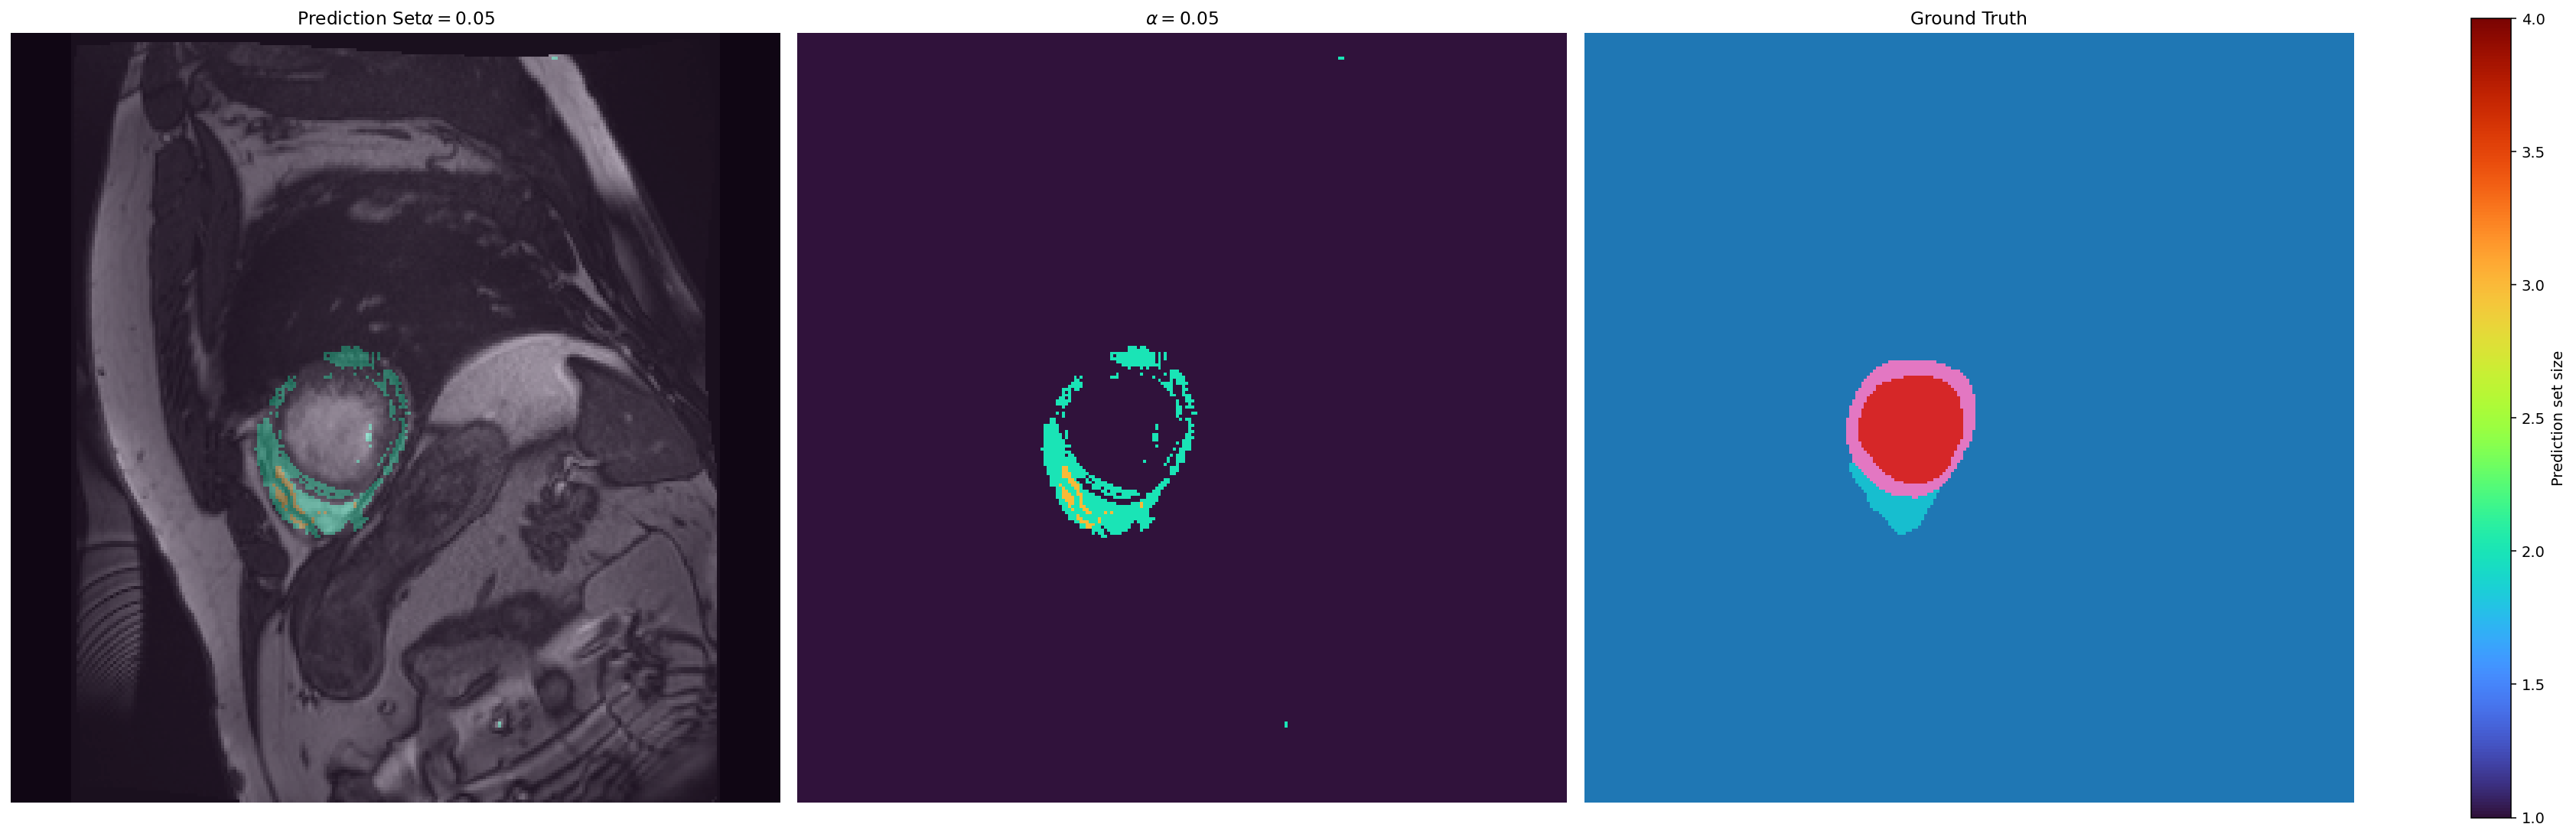
\includegraphics[width=1\linewidth]{img/prediccion_desv.png}
    \caption{Predicción, incerteza y grouth true}
    \label{fig:pred_desv}
\end{figure}

\begin{figure}[H]
    \centering
    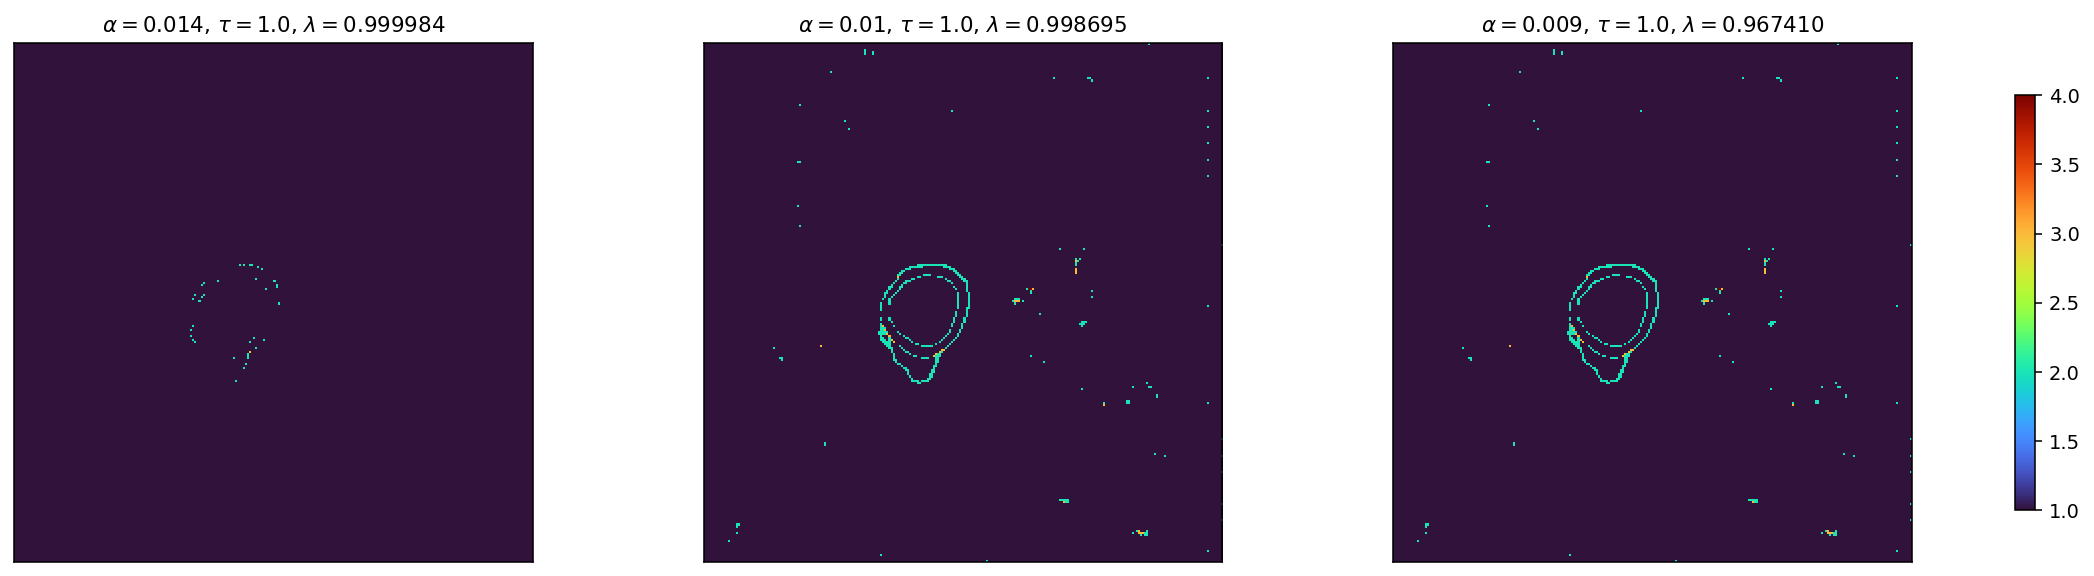
\includegraphics[width=1\linewidth]{img/variando_alphas.png}
    \caption{Incertidumbre del modelo para alphas [0.014, 0.01, 0.0090] y la temperatura $\tau = 1.0$ }
    \label{fig:desviacion_alphas}
\end{figure}

Las regiones de predicción se construyen agregando, píxel a píxel, todas las clases cuyas probabilidades predichas superen el umbral $1 - \hat{\lambda}$. Adicionalmente, se incluye de forma determinista la clase con la mayor probabilidad estimada en cada caso; esta modificación técnica previene la obtención de conjuntos vacíos en regímenes donde el umbral de aceptación resulta excesivamente estricto (valores de $\hat{\lambda}$ muy pequeños).


\section{TOA}
\subsection{Cuantificación de incertidumbre para imágenes médicas mediante FBPINN}

En esta sección se aborda la cuantificación de la incertidumbre en un conjunto de datos de imágenes de estructuras vasculares (venas). Estas imágenes fueron reconstruidas a través de un modelo de Redes Neuronales Informadas por la Física (PINN); en particular, se empleó la arquitectura de PINN Basada en Bases Finitas (FBPINN).

Como se describió previamente, la aplicación de la predicción conforme requiere definir inicialmente una función de puntuación de no conformidad. Para este propósito, se propone utilizar la norma $\mathbb{L}_1$, definida formalmente como:
\begin{equation}
    S = |y - \hat{y}|
\end{equation}

\begin{figure}[H]
    \centering
    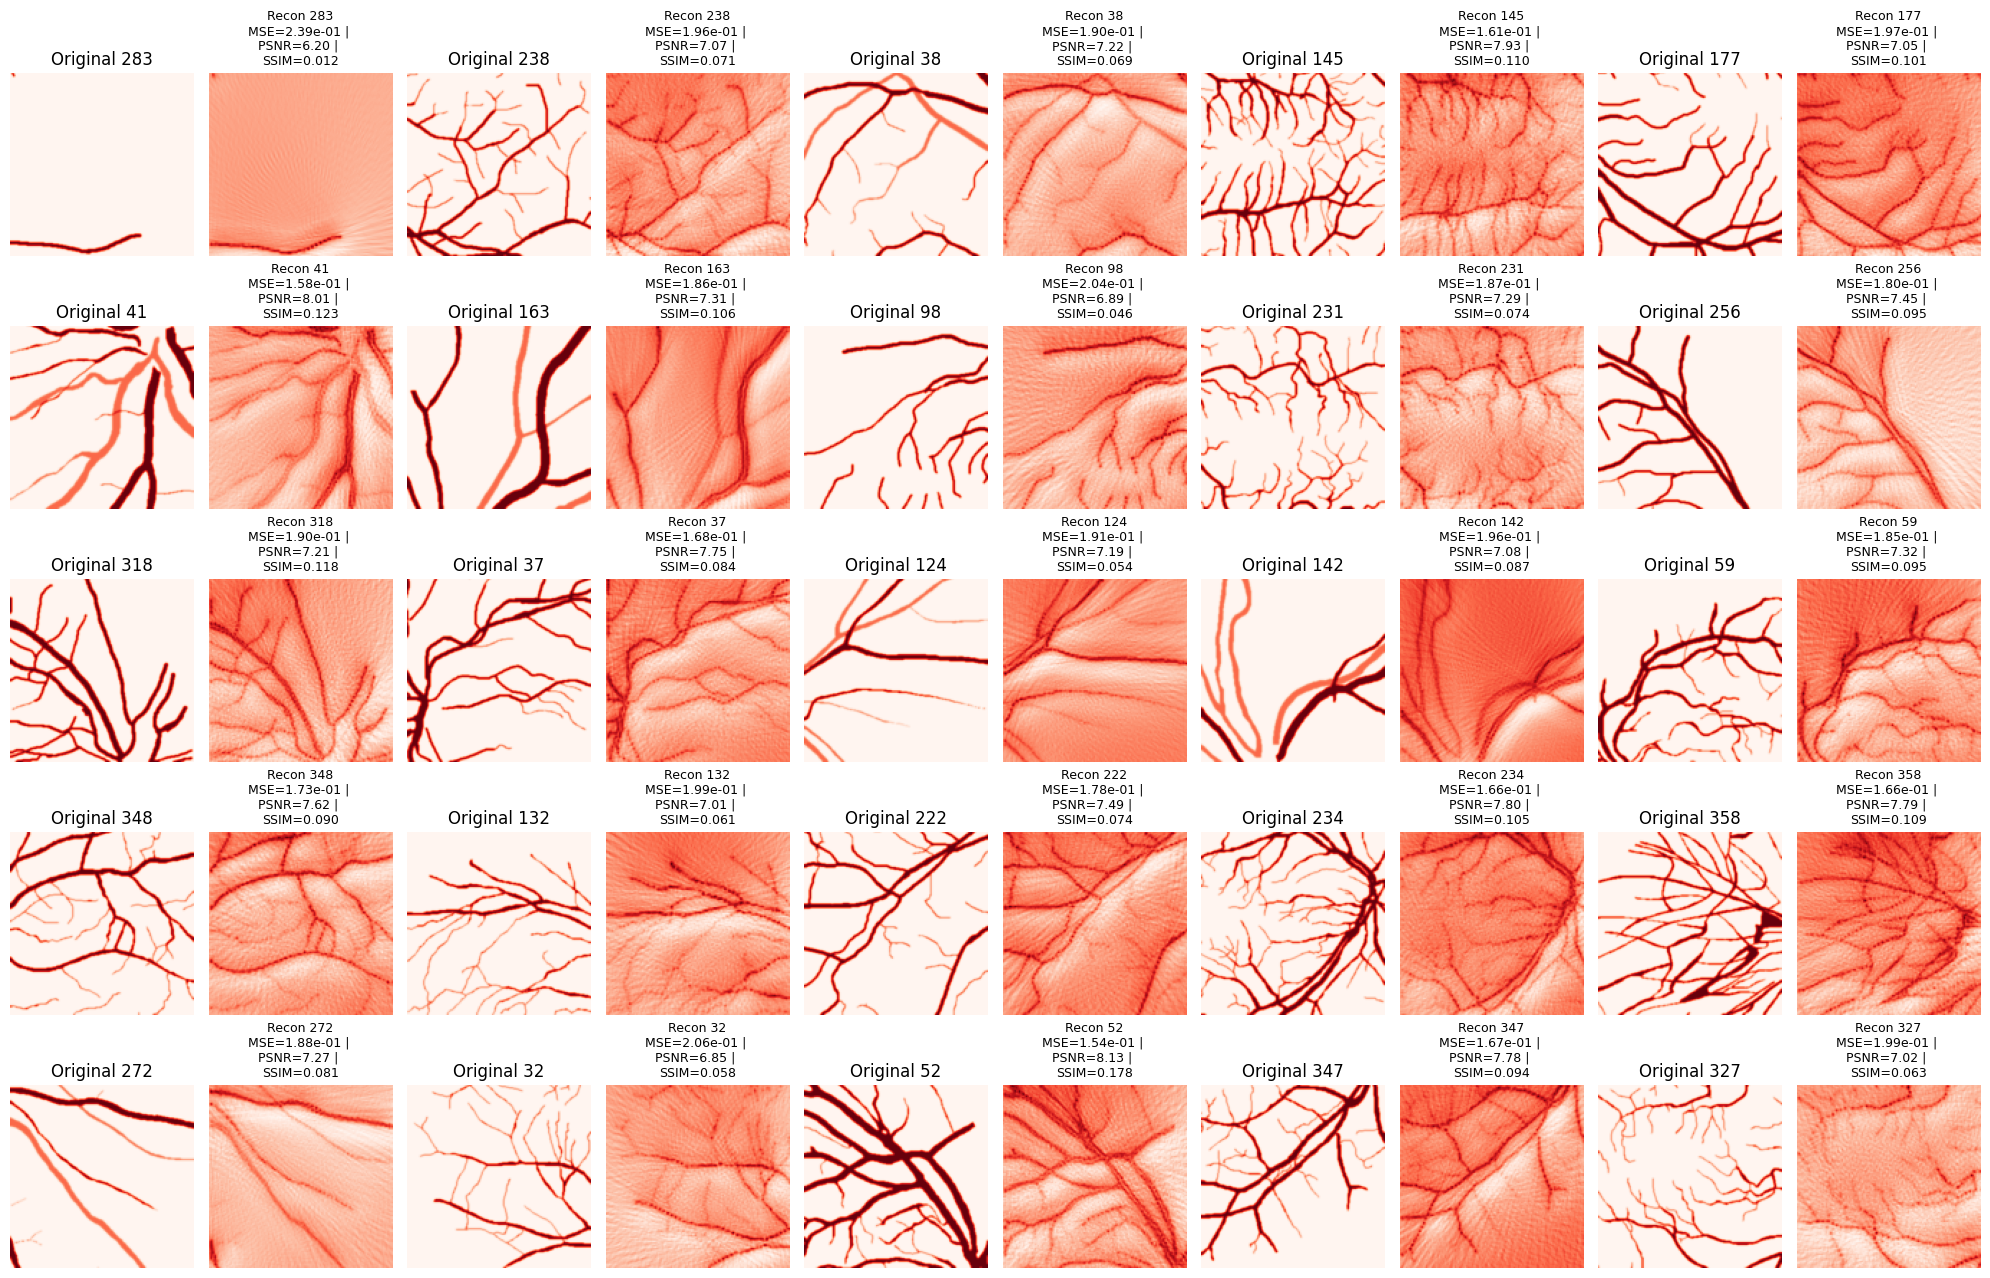
\includegraphics[width=1\linewidth]{img/data_init.png}
    \caption{Imágenes médicas reconstruidas mediante FBPINN y resolución del problema inverso.}
    \label{fig:data_fbpinn}
\end{figure}

Es fundamental destacar que el modelo no toma como entrada la imagen original directamente, sino una reconstrucción fundamentada en funciones gaussianas. El operador aprende a reconstruir la onda acústica a través del pulso gaussiano aplicándolo a cada coordenada espacial de la imagen, generando así un sinograma. Posteriormente, este sinograma es procesado por un algoritmo determinista que resuelve el problema inverso para reconstruir la imagen final.

Por lo tanto, la entrada efectiva al modelo se denota como $y_{\text{reconstruida}} = p_0$, la cual representa una matriz espacial con los valores de presión inicial para cada píxel. Sobre esta base, se procede a aplicar un conjunto de algoritmos de predicción conforme con carácter exploratorio.

\subsubsection{Split Conformal Prediction (SCP) en FBPINN}

En primera instancia, se evalúa el algoritmo SCP aplicado de forma independiente píxel a píxel, modalidad que se denota en la literatura como calibración condicional local. Es imperativo resaltar que el algoritmo SCP convencional ofrece, por definición, una garantía de cobertura marginal; es decir, el nivel de confianza se cumple en el promedio de la imagen y no necesariamente de manera condicional para cada píxel de forma aislada.

Para mitigar la varianza en la estimación de los cuantiles locales y aproximar una cobertura condicional robusta, se requiere disponer de un volumen considerable de muestras en el conjunto de calibración.

\begin{figure}[H]
    \centering
    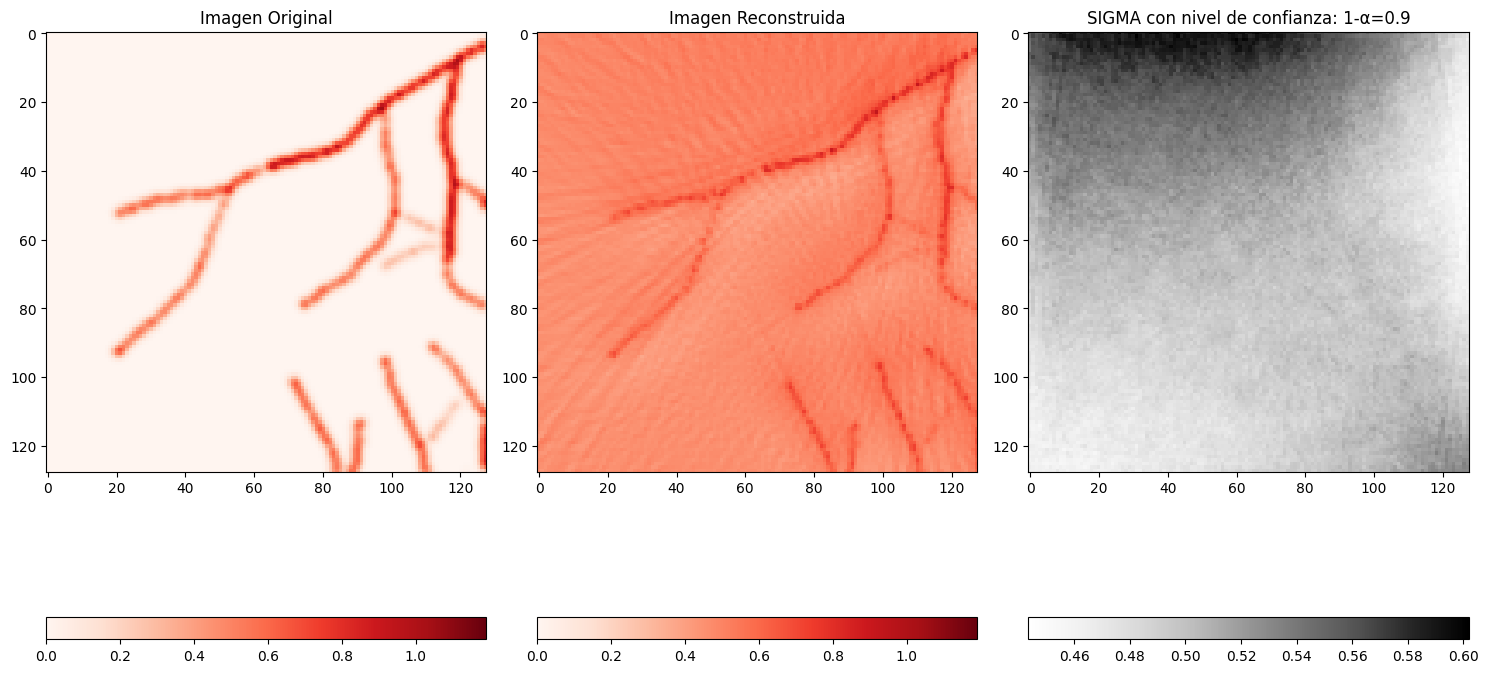
\includegraphics[width=0.8\linewidth]{img/scp_fbpinn.png}
    \caption{Split Conformal Prediction aplicado bajo calibración condicional, donde $\sigma = \hat{q}$.}
    \label{fig:scp_fbpinn}
\end{figure}

Un aspecto analítico relevante observado en la Figura~\ref{fig:scp_fbpinn} es que el umbral $\hat{q}$ deja de ser un escalar constante para todo el dominio. En su lugar, se transforma en una matriz que preserva la dimensión espacial de la imagen, de modo que $\hat{q} \in \mathbb{R}^{H \times W}$.

Esta técnica proporciona una caracterización topográfica general de la incertidumbre a lo largo de la malla de píxeles, permitiendo formular una región de predicción conforme de la forma $\hat{f}(X_{\text{test}}) \pm \hat{q}$. No obstante, estos intervalos de confianza resultan idénticos para cualquier instancia del conjunto de prueba $(\mathcal{X}, \mathcal{Y})_{\frac{n}{2} + 1, \dots, n}$, a pesar de que la física del problema sugiere que la incertidumbre debería exhibir variaciones dinámicas entre imágenes.

Con el objetivo de introducir dependencia de la muestra en la inferencia, e inspirándonos en el método de puntuación por residuo escalado, se propone una modificación adaptativa. Mientras que la etapa de calibración permanece invariante, la incertidumbre resultante para la fase de prueba se escala mediante la siguiente formulación:

\begin{equation}
    \sigma_q = \frac{q(i,j)^{\alpha}}{\mathcal{\hat{\pi}}(y \in \mathcal{R}_1|x)(i,j)}
\end{equation}

Donde el término $\mathcal{\hat{\pi}}(y \in \mathcal{R}_1|x)(i,j)$ representa la probabilidad condicional de que el píxel en la coordenada $(i,j)$ pertenezca a la estructura vascular (vena), $q(i,j)^{\alpha}$ es debido a que por cada $\alpha$ seteado se obtendrá una nueva matriz de $q(i,j)$.

Para estimar esta distribución, la imagen se segmenta mediante el algoritmo de Expectación-Maximización (EM) usando mezcla de gaussiandas  sobre el espacio de intensidades de los píxeles los cuales fueron clusterizados con y sin ecualización previa.

El proceso consiste en normalizar las intensidades del histograma al intervalo $[0, 255]$ para posteriormente ajustar el modelo de mixturas que infiere la probabilidad píxel a píxel. Esta probabilidad actúa como una máscara adaptativa que genera regiones de incertidumbre dinámicas y específicas para cada imagen de prueba.

\begin{figure}[H]
    \centering
    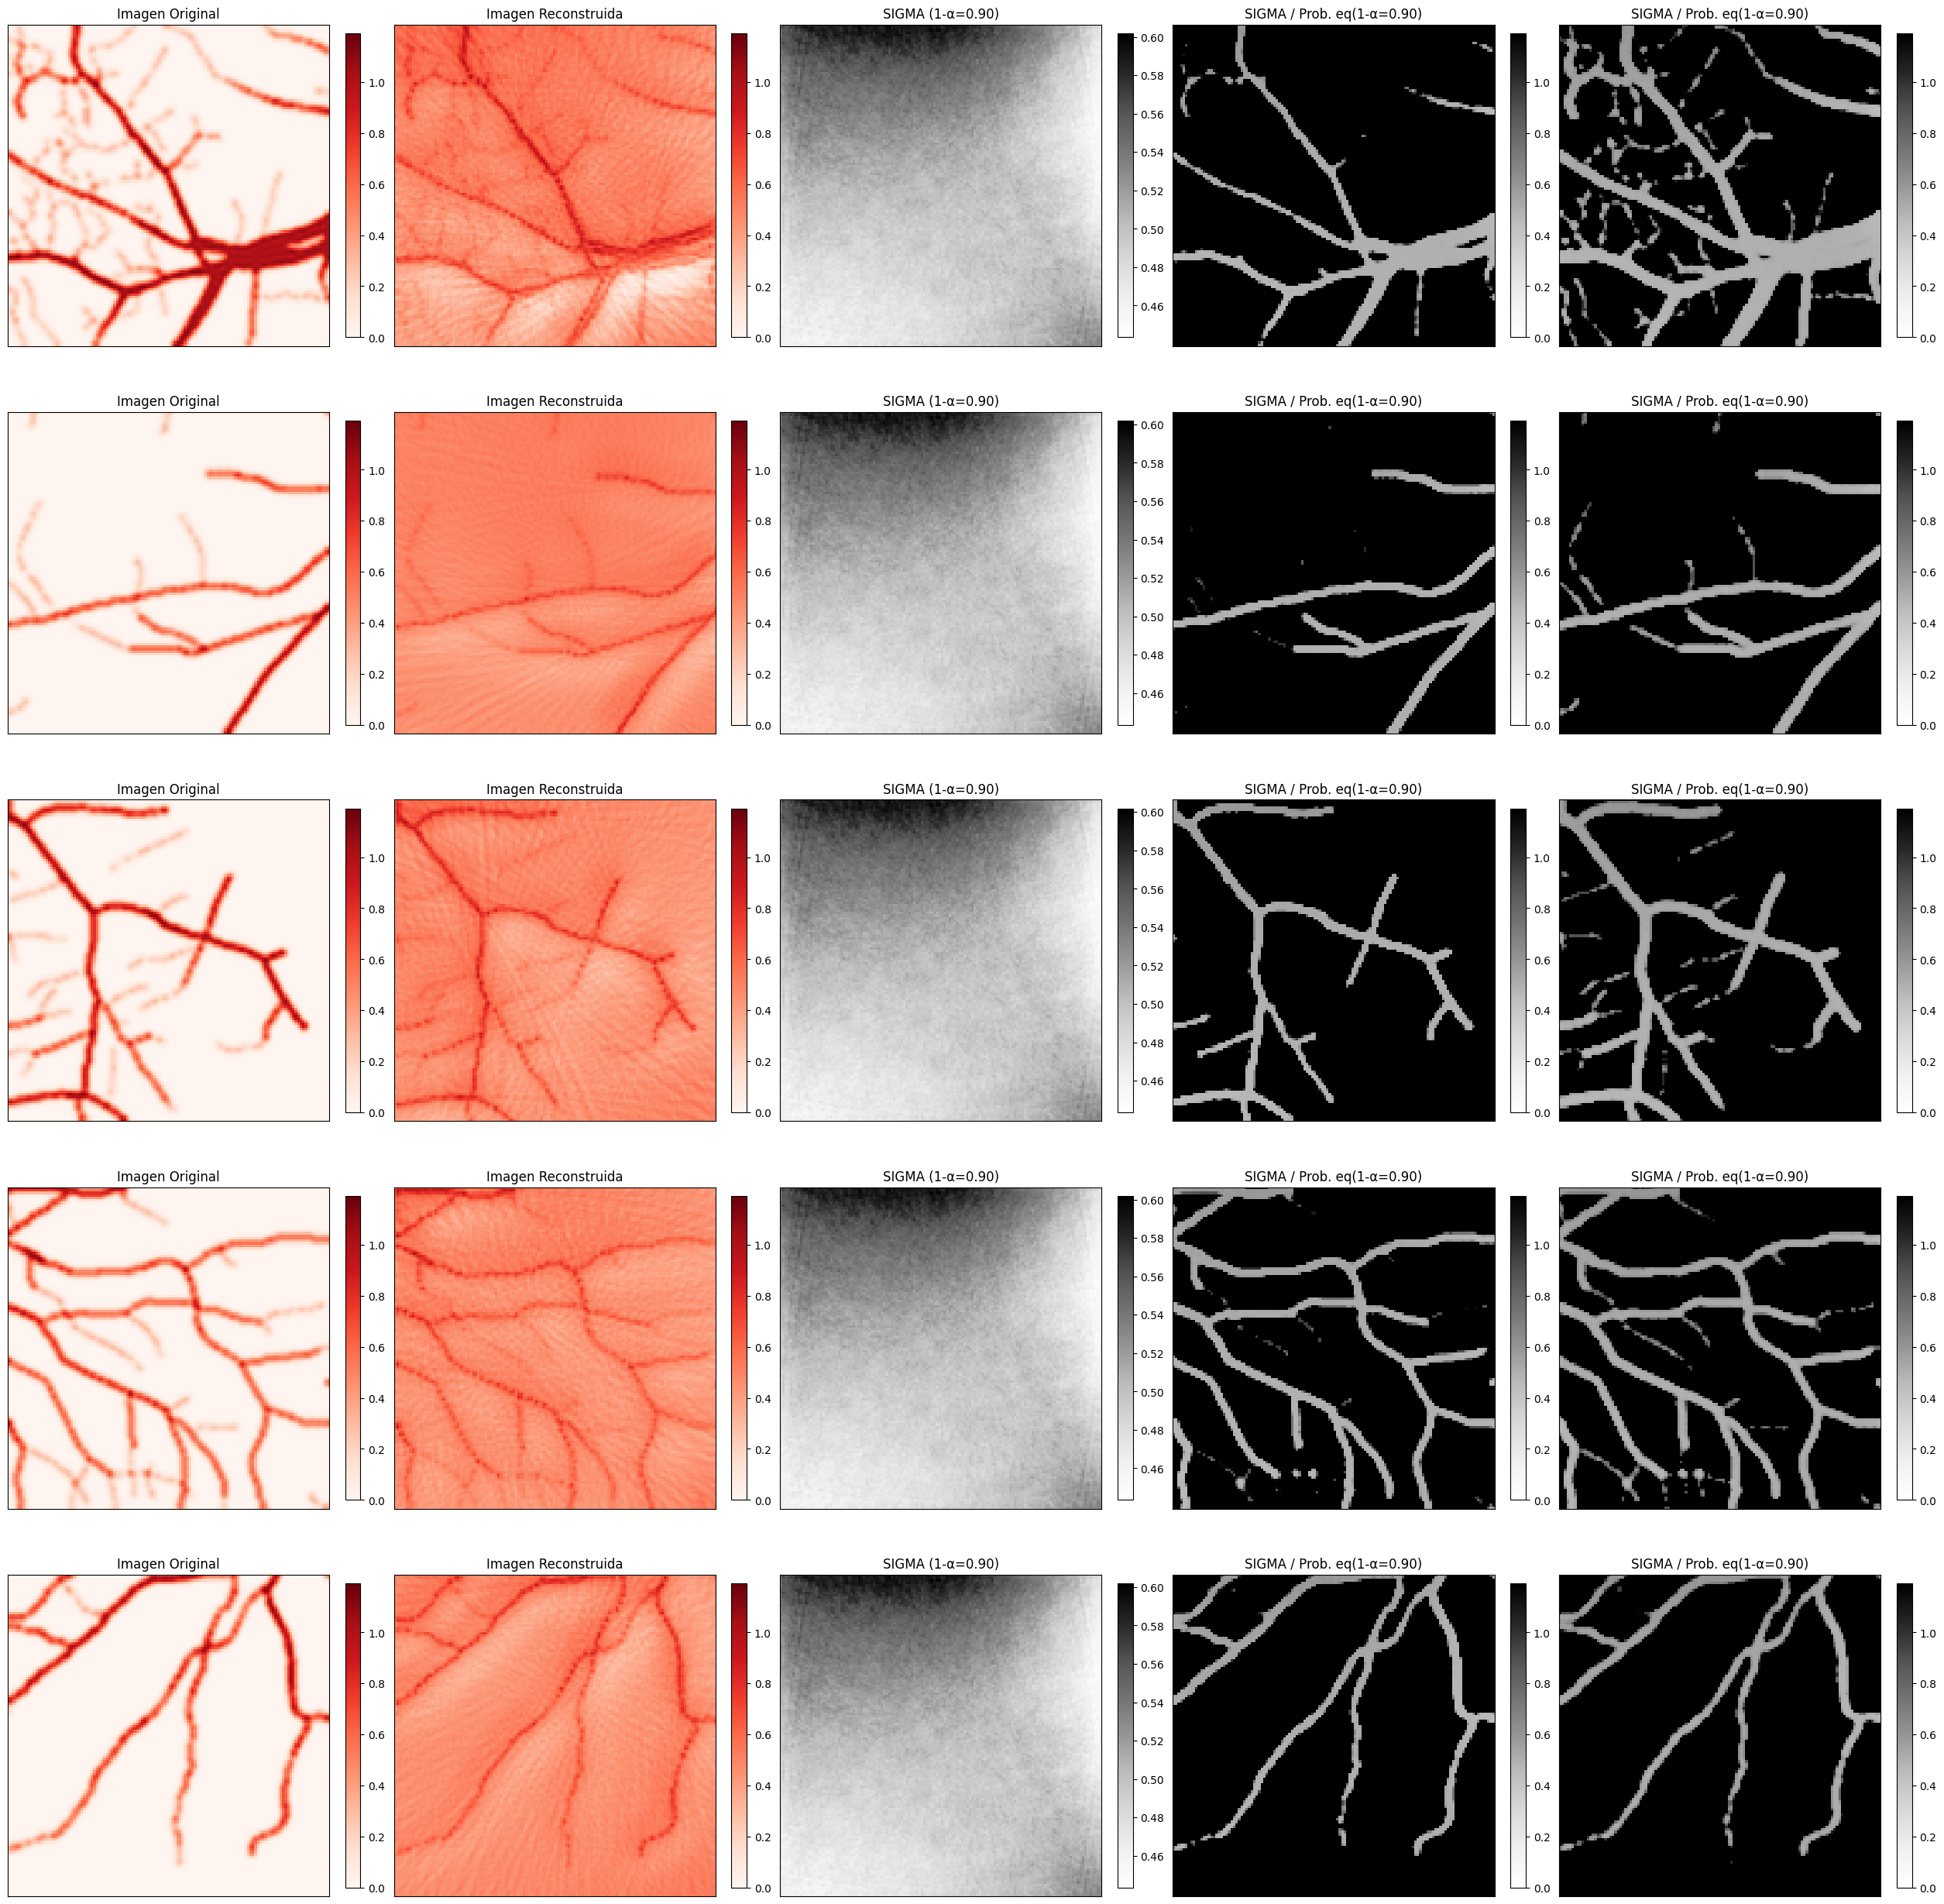
\includegraphics[width=0.75\linewidth]{img/scp_conf_EM.png}
    \caption{Split Conformal Prediction con bandas de predicción escaladas mediante la máscara de probabilidad EM.}
    \label{fig:scp_mascara}
\end{figure}

\subsubsection{SCP basado en partición binaria de clases}

A partir de la capacidad de segmentación introducida en el enfoque anterior, surge la oportunidad estratégica de fragmentar el dominio de calibración. Específicamente, se propone aplicar SCP condicional de forma aislada para el conjunto de píxeles clasificados como estructuras vasculares, y un proceso homólogo e independiente para los píxeles asignados al fondo.

Bajo este esquema, el dominio espacial se particiona en dos subconjuntos disjuntos a los cuales se les induce un proceso de calibración conforme por separado.

\begin{figure}[H]
    \centering
    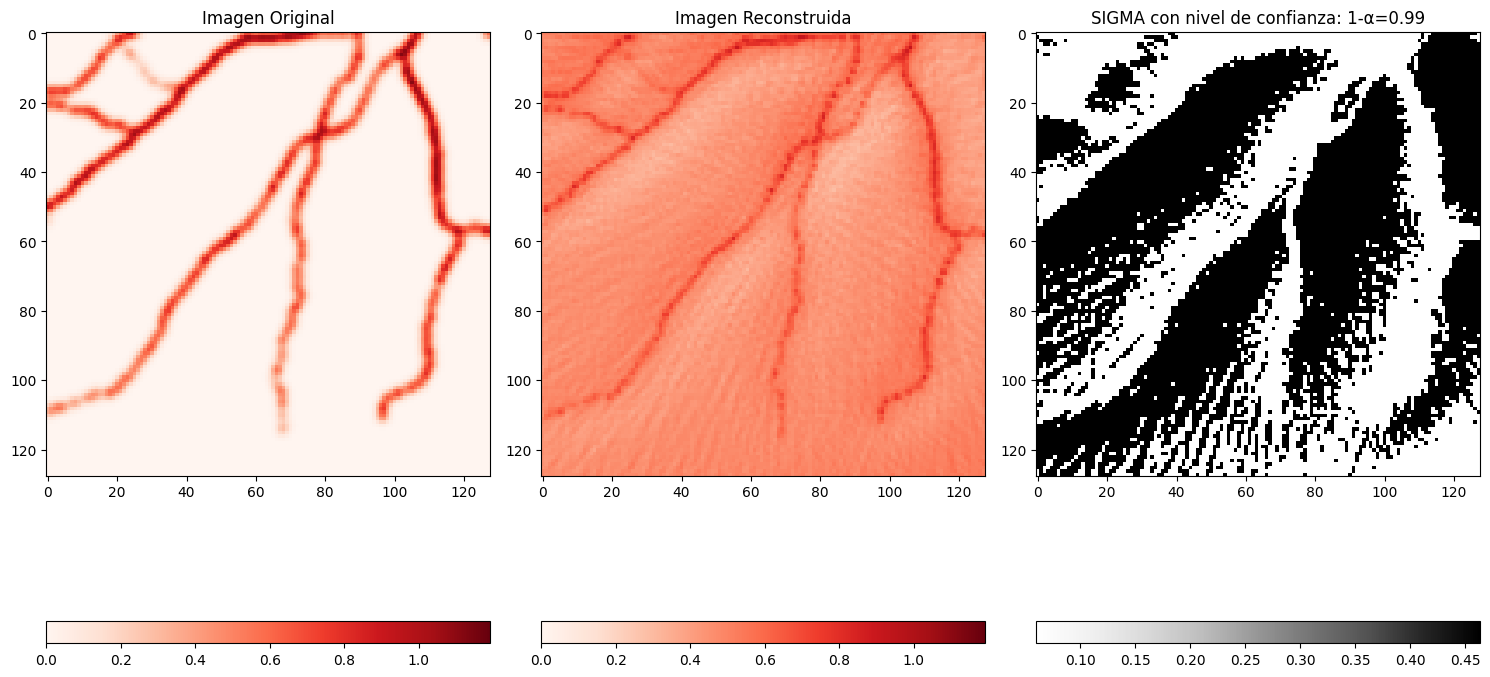
\includegraphics[width=0.75\linewidth]{img/scp_doble_em.png}
    \caption{Esquema de doble Split Conformal Prediction aplicado de forma independiente a las regiones de vena y fondo.}
    \label{fig:doble_scp_cluster}
\end{figure}

Este enfoque binario permite restringir el tamaño de los intervalos, logrando disminuir significativamente la incertidumbre en las regiones donde no se compromete la presencia de estructuras vasculares.

\subsubsection{Método de Kandinsky}

El método de Kandinsky, concebido originalmente para escenarios de clasificación, busca armonizar las ventajas de la calibración condicional local y la calibración marginal, tal como se detalla en el algoritmo~\ref{alg:kandinsky}. A través de un enfoque basado en agrupamiento espacial y pooling de puntuaciones de no conformidad, el método viabiliza estimaciones estables y estadísticamente válidas en dimensiones espaciales de alta resolución.

\begin{algorithm}[H]
    \caption{Algoritmo de Kandinsky Conformal Prediction}
    \label{alg:kandinsky}
    \begin{algorithmic}[1]
        \REQUIRE Tensor de no conformidad de calibración $\mathbf{S} \in \mathbb{R}^{N \times H \times W}$, niveles de cuantiles discretos $\mathcal{Q} = \{\tau_1, \dots, \tau_M\}$, número de clústeres $K$, nivel de significancia $\alpha$, instancia de prueba $X_{\text{test}}$.
        \ENSURE Mapa topográfico de umbrales $\mathbf{Q} \in \mathbb{R}^{H \times W}$, conjuntos de predicción válidos $\mathcal{C}_{\alpha}(X_{\text{test}})$.

        \vspace{0.1cm}
        \STATE \textbf{// Fase I: Extracción de Características Locales}
        \FOR{cada coordenada espacial $(i, j) \in \{1, \dots, H\} \times \{1, \dots, W\}$}
            \STATE Inicializar vector de perfil de riesgo: $\mathbf{x}_{i,j} \in \mathbb{R}^M$
            \FOR{$m = 1$ \TO $M$}
                \STATE $\mathbf{x}_{i,j}[m] \leftarrow \inf \left\{ q \in \mathbb{R} : \frac{1}{N} \sum_{n=1}^N \mathbb{I}(S_{n,i,j} \leq q) \geq \tau_m \right\}$
            \ENDFOR
        \ENDFOR
        \STATE Construir la matriz global de diseño: $\mathbf{X} \leftarrow \big[\mathbf{x}_{1,1}, \dots, \mathbf{x}_{H,W}\big]^T \in \mathbb{R}^{(H \cdot W) \times M}$

        \vspace{0.1cm}
        \STATE \textbf{// Fase II: Agrupamiento Espacial (Clustering)}
        \STATE Calcular la partición del dominio $\pi: \{1, \dots, H\} \times \{1, \dots, W\} \to \{1, \dots, K\}$ vía Clustering($\mathbf{X}, K$)
        \STATE Asignar la máscara estática de Kandinsky $\mathbf{M} \in \{1, \dots, K\}^{H \times W}$ tal que $\mathbf{M}_{i,j} \leftarrow \pi(i,j)$
Kandisnky2023
        \vspace{0.1cm}
        \STATE \textbf{// Fase III: Calibración Regional (Pooling)}
        \FOR{cada índice de clúster $k = 1$ \TO $K$}
            \STATE Agregar el multiconjunto de puntuaciones históricas: $\mathcal{S}_k \leftarrow \Big\{ S_{n,i,j} \;\Big|\; n \in \{1, \dots, N\}, \; \mathbf{M}_{i,j} = k \Big\}$
            \STATE Determinar el tamaño muestral efectivo regional: $N_k \leftarrow |\mathcal{S}_k| $
            \STATE Calcular el cuantil corregido: $q_k^* \leftarrow \inf \left\{ q \in \mathbb{R} : \frac{1}{N_k} \sum_{s \in \mathcal{S}_k} \mathbb{I}(s \leq q) \geq \frac{\lceil (N_k + 1)(1 - \alpha) \rceil}{N_k} \right\}$
        \ENDFOR

        \vspace{0.1cm}
        \STATE \textbf{// Fase IV: Inferencia Estática y Proyección}
        \STATE Proyectar mapa de umbrales: $\mathbf{Q}_{i,j} \leftarrow \sum_{k=1}^K q_k^* \cdot \mathbb{I}(\mathbf{M}_{i,j} = k) \quad \forall (i,j)$
        \FOR{cada píxel $(i, j) \in X_{\text{test}}$}
            \STATE $\mathcal{C}_{\alpha}(X_{\text{test}})_{i,j} \leftarrow \left\{ y \in \{1, \dots, \mathcal{Y}\} : 1 - \hat{f}(X_{\text{test}})_{i,j,y} \leq \mathbf{Q}_{i,j} \right\}$
        \ENDFOR

        \RETURN $\mathbf{Q}$, $\mathcal{C}_{\alpha}(X_{\text{test}})$
    \end{algorithmic}
\end{algorithm}

Si bien el algoritmo de Kandinsky fue concebido originalmente para problemas de clasificación, su formulación matemática permite extenderlo de manera directa al ámbito de la regresión. Dado que el método opera fundamentalmente sobre la distribución espacial de las puntuaciones de no conformidad, las funciones de score continuas provenientes de un regresor base pueden ser integradas y calibradas bajo los mismos principios de agregación regional y agrupamiento espacial descritos en las secciones anteriores.

\begin{figure}[H]
    \centering
    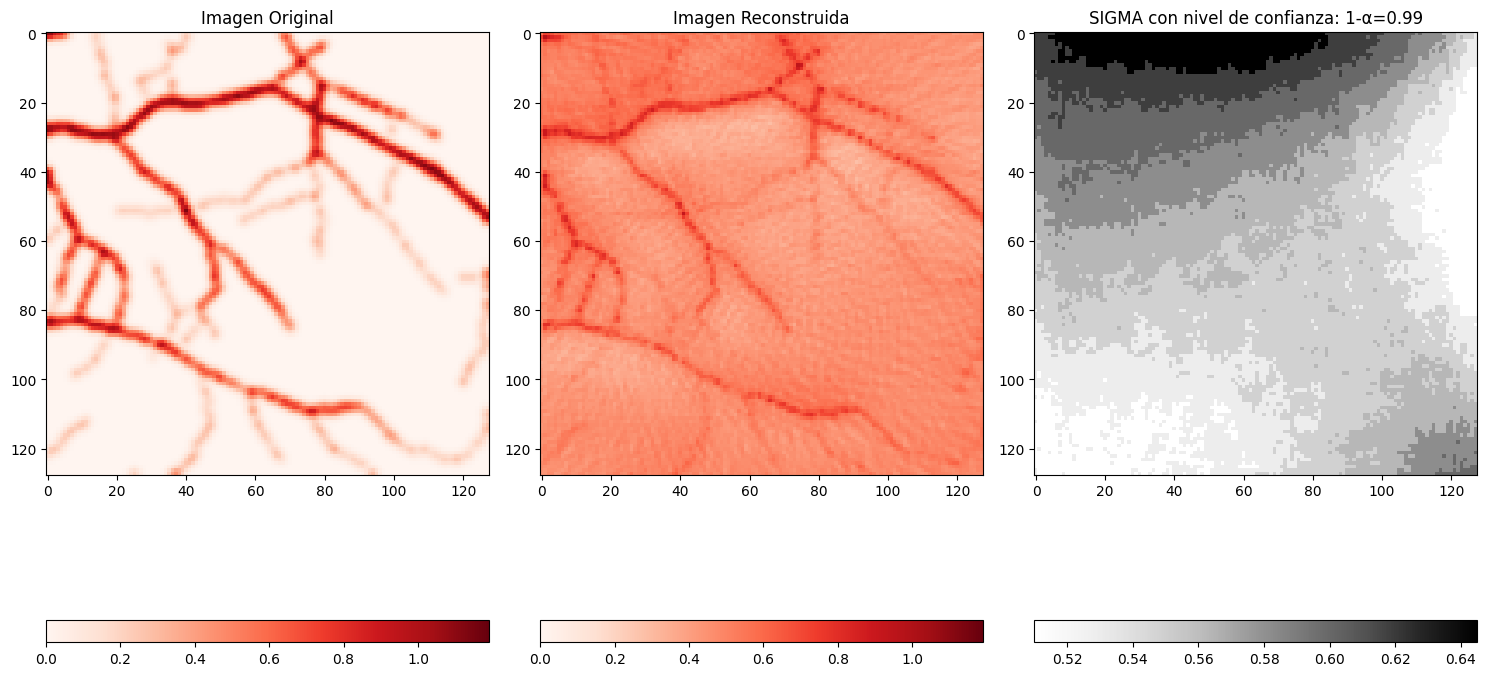
\includegraphics[width=0.75\linewidth]{img/kandinsky.png}
    \caption{Kandinsky conformal predictión}
    \label{fig:kandinsky}
\end{figure}


En la primera fase, el método condensa la información del conjunto de calibración calculando $M$ cuantiles empíricos de forma local para cada píxel. De este modo, se transforma el histórico dimensional de errores en una matriz espacial de características exógenas donde cada coordenada geométrica queda representada por un vector que describe su perfil de riesgo local.

Posteriormente, en la segunda fase, estos vectores de cuantiles actúan como las características de entrada para un algoritmo de agrupamiento parametrizado con $K$ clases, lo que permite segmentar y particionar el dominio de la imagen en una máscara estática que unifica los píxeles con dinámicas de incertidumbre estadísticamente similares.

En la tercera fase, se ejecuta un proceso de recalibración independiente sobre los componentes de cada clúster; al agregar las puntuaciones de no conformidad de todos los píxeles pertenecientes a una misma región a lo largo de todas las muestras de calibración, se produce un aumento masivo de datos que estabiliza el tamaño muestral efectivo. Este mecanismo de agregación regional no solo optimiza la precisión en la estimación del cuantil conforme global, sino que además mitiga de manera drástica el ruido heterocedástico local de alta frecuencia.

Finalmente, durante la etapa de inferencia, la predicción de cualquier instancia futura se realiza proyectando los scores del modelo sobre el mapa de umbrales estáticos e invariantes derivado de los datos aumentados, garantizando así la estabilidad y robustez de la cobertura condicional por zona.

\section{THz}
Kandisnky2023





\chapter{Conclusiones}

\appendix
\chapter{Anexo}

\section{Teorema 1}
\label{anexo:teorema1}

Supongamos que $(X_i, Y_i)_{i=1,\dots,n}$ y $(X_\text{test}, Y_\text{test})$ son i.i.d. Entonces definimos $\hat{q}$ como
\begin{equation*}
\hat{q} = \inf \Bigg\{ q : \frac{\left| \{i : s(X_i, Y_i) \leq q\} \right|}{n} \;\ge\; \frac{\lceil (n + 1)(1 - \alpha)\rceil}{n} \Bigg\},
\end{equation*}
y los conjuntos de predicción resultantes como
\begin{equation*}
C(X) = \{y : s(X, y) \leq \hat{q}\}.
\end{equation*}
Entonces,
\begin{equation*}
\mathbb{P}\big(Y_\text{test} \in C(X_\text{test})\big) \;\ge\; 1 - \alpha.
\end{equation*}
Esta es la misma propiedad de cobertura que la ecuación (1) en la introducción, pero escrita de forma más formal.

Como observación técnica, el teorema también se cumple si las observaciones satisfacen la condición más débil de \textbf{intercambiabilidad} (\textit{exchangeability}); ver [1]. A continuación, probamos la cota inferior.

\vspace{0.3cm}
\begin{proof}[Prueba del Teorema 1]
Sea $s_i = s(X_i, Y_i)$ para $i=1,\dots,n$ y $s_\text{test} = s(X_\text{test}, Y_\text{test})$. Para evitar manejar empates, consideramos el caso en el cual los $s_i$ son distintos con probabilidad 1. Ver [25] para una prueba en el caso general.

Sin pérdida de generalidad, asumimos que los puntajes de calibración están ordenados de modo que
\begin{equation*}
s_{(1)} < \cdots < s_{(n)}.
\end{equation*}
En este caso, tenemos que
\begin{equation*}
\hat{q} =
\begin{cases}
    s_{(\lceil (n+1)(1-\alpha)\rceil)} & \text{si } \alpha \ge \frac{1}{n+1}\\
    \infty & \text{e.o.c.}
\end{cases}
\end{equation*}
Notemos que, en el caso $\hat{q} = \infty$, se cumple $C(X_\text{test}) = \mathcal{Y}$, por lo que la propiedad de cobertura se satisface trivialmente; así que solo debemos tratar el caso $\alpha \ge 1/(n+1)$.

Procedemos observando la igualdad de los dos eventos:
\begin{equation*}
\{Y_\text{test} \in C(X_\text{test})\} = \{s_\text{test} \leq \hat{q}\}.
\end{equation*}
Combinando esto con la definición de $\hat{q}$, obtenemos:
\begin{equation*}
\{Y_\text{test} \in C(X_\text{test})\} = \{s_\text{test} \leq s_{(\lceil (n+1)(1-\alpha)\rceil)}\}.
\end{equation*}
Aquí viene la idea crucial. Por la intercambiabilidad de las variables $(X_1,Y_1), \dots, (X_\text{test},Y_\text{test})$, tenemos:
\begin{equation*}
\mathbb{P}(s_\text{test} \leq s_{(k)}) = \frac{k}{n+1}, \quad \text{para todo entero } k.
\end{equation*}
En palabras, $s_\text{test}$ es igualmente probable de caer en cualquier posición entre los puntos de calibración $s_{(1)},\dots,s_{(n)}$. Nótese que aquí la aleatoriedad es sobre todas las variables $s_1,\dots,s_n,s_\text{test}$.

De aquí concluimos lo siguiente. Tomando $k=\lceil (n+1)(1-\alpha)\rceil$, se tiene:
\begin{equation*}
\mathbb{P}\big(s_{\text{test}}\le s_{(k)}\big)=\frac{k}{n+1} =\frac{\lceil (n+1)(1-\alpha)\rceil}{n+1}\ge\frac{(n+1)(1-\alpha)}{n+1}=1-\alpha.
\end{equation*}
De ahí se obtiene la cota inferior de cobertura:
\begin{equation*}
\mathbb{P}(Y_{\text{test}}\in C(X_{\text{test}}))=\mathbb{P}(s_{\text{test}}\le\hat{q}) \ge 1-\alpha.
\end{equation*}
\end{proof}

\vspace{0.2cm}
Ahora la cota superior. Técnicamente, la cota superior solo se cumple cuando la distribución del score conforme es continua, evitando empates. En la práctica, sin embargo, esta condición no es importante, porque el usuario siempre puede añadir una cantidad ínfima de ruido aleatorio al score.

\vspace{0.3cm}
\noindent\textbf{Teorema D.2} (\textit{Cota superior de la calibración conforme}). \textit{Adicionalmente, si los puntajes $s_1,\dots,s_n$ tienen una distribución conjunta continua, entonces}
\begin{equation*}
\mathbb{P}\big(Y_\text{test} \in C(X_\text{test}, U_\text{test}, \hat{q})\big) \;\le\; 1 - \alpha + \frac{1}{n+1}.
\end{equation*}

\begin{thebibliography}{ABJ24}

\bibitem[AB21]{angelopoulos2021gentle}
A. N. Angelopoulos y S. Bates.
\newblock {\em A Gentle Introduction to Conformal Prediction}.
\newblock arXiv preprint arXiv:2107.07511, 2021.
\newblock \url{https://arxiv.org/abs/2107.07511}.

\bibitem[ABJ24]{angelopoulos2024conformal}
A. N. Angelopoulos, Rina Foygel Barber2, Stephen Bates.
\newblock {\em Theoretical Foundations of Conformal Prediction}.
\newblock arXiv preprint arXiv:2411.11824, 2024.
\newblock \url{https://arxiv.org/abs/2411.11824}.



\bibitem[VGB24]{segment_cp_2024}
A. Varisco, L. Galteri, S. Bruni y A. Del Bimbo.
\newblock {\em Conformal Semantic Image Segmentation: Post-hoc Quantification of Predictive
Uncertainty}.
\newblock arXiv preprint arXiv:2405.05145, 2024.
\newblock \url{https://arxiv.org/abs/2405.05145}.



\bibitem[SML24]{stml2024intro}
Scientific Machine Learning.
\newblock {\em Introduction to Conformal Prediction}.
\newblock Plataforma interactiva de documentación, 2026.
\newblock \url{https://scientific-machine-learning.streamlit.app/intro_cp}.


\bibitem[KCP]{Kandisnky2023}
Scientific Machine Learning.
\newblock {\em Kandinsky Conformal Prediction: Efficient Calibration of Image
Segmentation Algorithms}.
\newblock arXiv preprint arXiv:2311.11837, 2023.
\newblock \url{https://arxiv.org/pdf/2311.11837}.

\bibitem[MDL]{DiLiscia2026}
Scientific Machine Learning.
\newblock {\em Redes Neuronales Guiadas para Aplicaciones Modeladas por la Ecuación de Onda}.
\newblock ---
\newblock \url{h---}.


\bibitem[MG]{MGonzales2024}
Scientific Machine Learning.
\newblock {\em DIFFUSION ASSISTED IMAGE RECONSTRUCTION IN
OPTOACOUSTIC TOMOGRAPHY}.
\newblock arXiv preprint arXiv:2404.10239
\newblock \url{https://arxiv.org/pdf/2404.10239}.

\bibitem[YY]{Yifan2025}
Yifan Yu, Cheuk Hin Ho, Yangshuai Wang,
\newblock {\em A conformal prediction framework for uncertainty quantification in physics-informed neural networks}.
\newblock arXiv preprint arXiv:2509.13717
\newblock \url{https://arxiv.org/pdf/2509.13717}.






\bibitem[BM]{BMosley2020}
B.Moseley, A.Markham y T.Nissen-Meyer
\newblock {\em Solving the wave equation with physics-informed deep learning}.
\newblock arXiv preprint arXiv:2006.11894
\newblock \url{https://arxiv.org/pdf/2006.11894}.



\bibitem[H91]{Hertz1991}
Anders Krogh, John Hertz y Richard G. Palmer
\newblock {\em Introduction To The Theory Of Neural Computation}.
\newblock url={https://books.google.co.cr/books?id=HlwZyAEACAAJ}.


\bibitem[M93]{universal1993}
Moshe Leshno and Vladimir Ya. Lin and Allan Pinkus and Shimon Schocken
\newblock {\em Multilayer feedforward networks, Activation functions, Role of threshold, Universal approximation capabilities, ($\mu$) approximation}.
\newblock url = {https://www.sciencedirect.com/science/article/pii/S0893608005801315}.

\bibitem[OR15]{unet2015}
Olaf Ronneberger, Philipp Fischer, and Thomas Brox
\newblock {\em U-Net: Convolutional Networks for Biomedical
Image Segmentation}.
\newblock url = {https://arxiv.org/pdf/1505.04597}.



\bibitem[DL26]{tesisDiliscia}
Matías Di Liscia
\newblock {\em Redes Neuronales Guiadas para Aplicaciones Modeladas por la Ecuación de Onda}.
\newblock url = {https://-----}.


\bibitem[VV12]{vock2012}
Vladimir Vovk
\newblock {\em Conditional validity of inductive conformal predictors}.
\newblock url = {https://arxiv.org/pdf/1209.2673}.


\bibitem[SLW18]{sadinle2018}
Mauricio Sadinle, Jing Lei, and Larry Wasserman
\newblock {\em Least Ambiguous Set-Valued Classifiers
with Bounded Error Levels}.
\newblock url = {https://arxiv.org/pdf/1609.00451}.



\end{thebibliography}

\end{flushleft}
\end{document}









%ref
% https://tikz.dev/editor/web/